\section{Benchmark Specifications}

%%%%%%%%%%%%%%%%%%%%%%%%%%%%%%%%%%%%%%%%%%%%%%%%%%%%%%%%%%%%%%%%%%%%%%%%%%%%%%%%
\subsection{Overview}

The core geometry specifications are described in 3 levels of increasing scope,
detailing each of the hierarchical elements of the model. First the radial
geometry is described, followed by a section detailing the axial parameters.

At the lowest level, the radial geometry of each of the pincell types used
throughout the core is described. Next, the fuel assembly design is detailed, 
including the possible configurations of burnable absorbers and the radial
specification of the grid spacers. Finally, the greater core geometry is
described, including the fuel assembly enrichment locations, the positions of
burnable absorbers, instrument tubes, control rod banks, and shutdown banks, as
well as the baffle that surrounds the fuel assemblies, the core barrel, four
neutron shield panels, and the reactor pressure vessel and liner.

After the radial and axial geometry descriptions, a material specifications
section lists the details of each of the materials referred to.
%Finally, the last section details the approximations made by this model and
%suggests addition approximations that might be appropriate.
Table \ref{overview_table} provides a summary of key model parameters that will
be specified in greater detail in subsequent sections, and Figure
\ref{fig_overview} shows a core cross section indicating the radial structures
and assembly loading pattern.
\newpage
\begin{table}
  \centering
  \caption{Summary of key model parameters. \label{overview_table}}
  \begin{tabularx}{\textwidth}{l C c}
    \toprule
    \multicolumn{3}{c}{\phantom{Source}\hfill Core Lattice \hfill Source}\\
    \midrule
    \midrule
    & & \\
    
    No. Fuel Assemblies & 193 & \ref{num:assycore}\\
    & & \\
    Loading Pattern & w/o U235 & \\
    ~~Region 1 (cycle 1) & 1.60$^\dagger$ & \ref{num:assycore}\\
    ~~Region 2 (cycle 1) & 2.40$^\dagger$ & \ref{num:assycore}\\
    ~~Region 3 (cycle 1) & 3.10$^\dagger$ & \ref{num:assycore}\\
    ~~Region 4A (cycle 2) & 3.20$^{\dagger\dagger}$ & \ref{num:assycore}\\
    ~~Region 4B (cycle 2) & 3.40$^{\dagger\dagger}$ & \ref{num:assycore}\\
    & & \\
    
    Cycle 1 Heavy Metal Loading & 81.8 MT & \ref{num:assyload} \\
    & & \\
    \midrule 
    \multicolumn{3}{c}{Fuel Assemblies}\\
    \midrule
    \midrule
    & & \\
    
    Pin Lattice Configuration & $17 \times 17$ & \ref{num:fuellattice}\\
    Active Fuel Length & 365.76 cm & \ref{num:fuelheight}\\
    No. Fuel Rods & 264 & \ref{num:fuellattice}\\
    No. Grid Spacers & 8 & \ref{num:fuellattice}\\
    
    & & \\
    \midrule
    \multicolumn{3}{c}{Control}\\
    \midrule
    \midrule
    & & \\
    
    Control Rod Material (Upper Region) & \hyperlink{mat_b4c_rod}{B4C} & \ref{num:b4c_rod_mat}\\
    Control Rod Material (Lower Region) & \hyperlink{mat_aic_rod}{Ag-In-Cd} & \ref{num:aic_rod_mat}\\
    No. Control Rod Banks & 57 & \ref{num:assycore}\\
    
    & & \\
    No. Burnable Poison Rods in Core & 1266 & \ref{num:assycore}\\
    Burnable Poison Material & \hyperlink{mat_borosilicate}{Borosilicate Glass}, 12.5 w/o $\mathrm{B}_2\mathrm{O}_3$ & \ref{num:fuellattice}\\
    
    & & \\
    \midrule
    \multicolumn{3}{c}{Performance}\\
    \midrule
    \midrule
    & & \\
    
    Core Power & 3411 MWth & \ref{num:measurement}\\
    Operating Pressure & 2250 psia & \ref{num:measurement}\\
    Core Flow Rate & $61.5\times10^6\,\mathrm{kg/hr}$ (5\% bypass$^\ddagger$) & \ref{num:flowrate} \\
    \bottomrule 
  \end{tabularx}
  \begin{small}\begin{flushleft}
    \noindent $^\dagger$ Cycle 1 Actual core-averaged enrichments calculated from detailed assembly loadings, see Source \ref{num:assy_load}. \\
    \noindent $^{\dagger\dagger}$ Cycle 2 Actual core-averaged enrichments calculated from detailed assembly loadings, see Source \ref{num:assy_load_c2}. \\
    \noindent $^\ddagger$ It is assumed that 5\% of core flow rate goes core into bypass region. A fraction of this flow rate passes through
                          guide tubes. The flow rate should be estimated so that no boiling occurs in these regions.
  \end{flushleft}\end{small}
\end{table}
\clearpage
\begin{figure}[hptb]
  \centering
  
  \begin{tikzpicture}[x=1cm, y=1cm]

    \def\sqrttwo{1.4142135624}
  
    % actual dimensions in cm
    \def\coreBarrelOR{193.6750}
    \def\rpvOR{241.300}
    \def\rpvIR{219.710}
    \def\shieldOR{201.630}
    \def\baffleOR{163.4998}  % lattice pitch * 7.5 + baffle width  (21.50364*7.5+2.2225)

    \def\figwidth{10.16} % figure width in cm, assumes figure is cropped to rpvOR
  
    % all the dimensions set based on fig being inculded as 4in
    \draw[white] (-6,-6) rectangle (6,6);
    \node {\pgftext{\includegraphics[width=\figwidth cm]{specifications/figs/pwr_core.png}}};
    \draw[red,thick,->]  (-2*2.54,2*2.54) node[left, anchor=south] {Pressure Vessel} --  (-\figwidth/2/\sqrttwo,\figwidth/2/\sqrttwo);
    \draw[red,thick,->]  (2*2.54,2*2.54) node[right, anchor=south] {Neutron Shield Panel} --  (\shieldOR*\figwidth/2/\rpvOR/\sqrttwo,\shieldOR*\figwidth/2/\rpvOR/\sqrttwo);
    \draw[red,thick,->]  (0,2.3*2.54) node[above, anchor=south] {Core Barrel} --  (0,\coreBarrelOR/\rpvOR*\figwidth/2);
    \draw[red,thick,->]  (-2.3*2.54,0) node[left, anchor=east] {Baffle} --  (-\baffleOR/\rpvOR*\figwidth/2,0);
    \draw[red,thick,->]  (2.3*2.54,0) node[right, anchor=west] {RPV Liner} --  (\rpvIR/\rpvOR*\figwidth/2,0);
    
  \end{tikzpicture}
  
  \caption[Core cross-section]{Core cross-section indicating radial structures
  and enrichment loading pattern (cycle 1). Black denote stainless steel, dark
  gray denotes carbon steel, light blue denotes water, and red, yellow, and dark
  blue denote the 1.6, 2.4, and 3.1 w/o U235 regions, respectively.
  \label{fig_overview}}
\end{figure}



%%%%%%%%%%%%%%%%%%%%%%%%%%%%%%%%%%%%%%%%%%%%%%%%%%%%%%%%%%%%%%%%%%%%%%%%%%%%%%%%
\subsection{Radial Geometry}

  \subsubsection[Pin Types]{Pin Types\texorpdfstring{\protect\sechypt{sec_pintypes}{}}{}}
\label{sec:pintypes}

In this section the radial parameters of each of the pincell types used in the
fuel assemblies are detailed. Each of these describes a complete pincell
surrounded by the main coolant - in other words, the outer guide tube shell that
surrounds instrument tubes, control rods, and burnable absorber rods is
presented here as part of those pincells.

While the following radial parameters are constant throughout the axial extent
of the core of most pins, a distinction is made for the pins that have
components below the control rod stop at the bottom of the core. This region,
referred to as the ``dashpot'', consists of a tapering of the guide tubes to a
thinner radius that causes the constriction of flow to naturally prevent control
rods from extending too far into the core. In this model, this is approximated
by a region of thinner guide tubes (described further in later sections). Thus
radial parameters are provided for pins for both regions where appropriate. Note
that the central guide tubes of each assembly (the "instrument tubes") do not
shrink for the dashpot.

For all figures in this section, dimensions and materials are specified in order
starting from the inner region, through the outer rings. No thermal expansion is
considered.

\begin{geoitem}{Fuel Pin}{fig_fuel_pin}\centering
  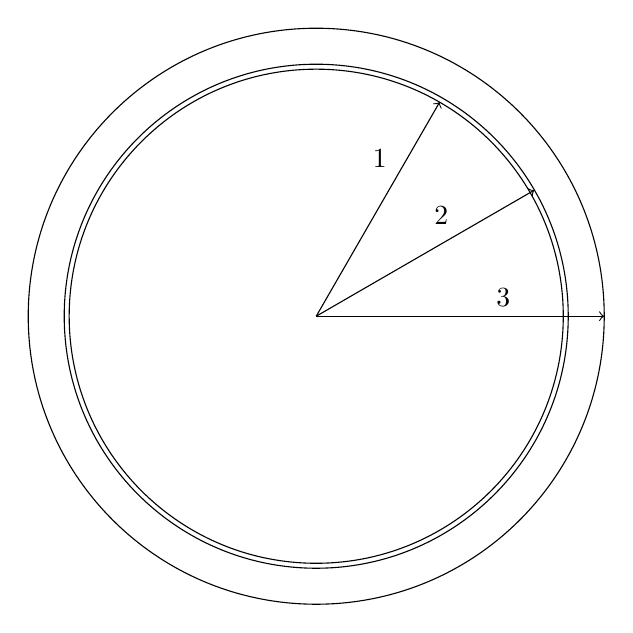
\begin{tikzpicture}[scale=8,auto]
        \draw (0,0) circle (0.39218);
      \draw[->] (0,0) -- node[pos=0.65] {1} (0.196,0.34);
      \draw (0,0) circle (0.40005);
      \draw[->] (0,0) -- node[pos=0.65] {2} (0.346,0.2);
      \draw (0,0) circle (0.4572);
      \draw[->] (0,0) -- node[pos=0.65] {3} (0.457,0.0);

      \end{tikzpicture}
      \begin{tikzpicture}
       \matrix [matrix of nodes]
      {
          Arrow & Radius (cm) & Material & \numrefheader \\
        1 & 0.39218 & \node[hyperlink node=mat_fuel16]{Fuel}; & \ref{num:fuelpellrad}\\ 
        2 & 0.40005 & \node[hyperlink node=mat_helium]{Helium}; & \ref{num:fuelIRrad}\\ 
        3 & 0.45720 & \node[hyperlink node=mat_zirc]{Zircaloy}; & \ref{num:fuelORrad}\\ 
      };
\end{tikzpicture}
\end{geoitem}
\begin{geoitem}{Upper Fuel Pin Plenum}{fig_fuel_pin_plenum}\centering
\input{specifications/pin/figs/tikz_fuel_plenum}
\\ \raggedright This shows the radial geometry used in the upper
plenum region of the fuel pins, with a small mass of Inconel to approximate the
spring.
\end{geoitem}

\begin{geoitem}{Empty Guide Tube Geometry above Dashpot}{fig_guidetube_pin}\centering
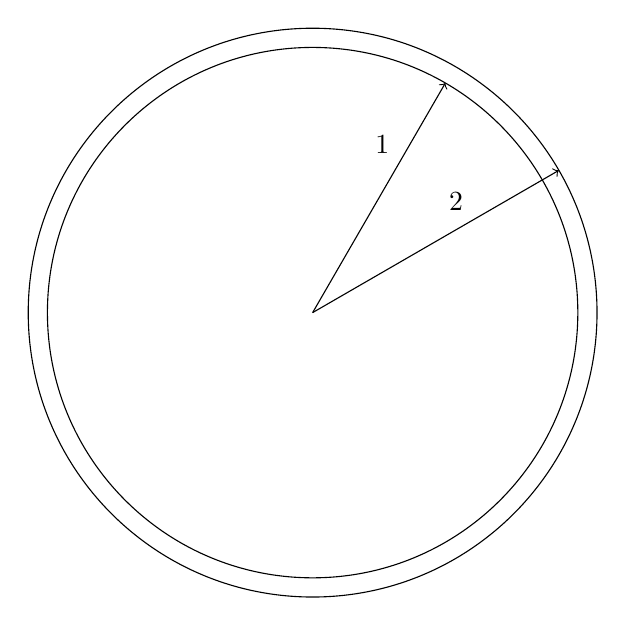
\begin{tikzpicture}[scale=6,auto]
        \draw (0,0) circle (0.56134);
      \draw[->] (0,0) -- node[pos=0.65] {1} (0.281,0.486);
      \draw (0,0) circle (0.60198);
      \draw[->] (0,0) -- node[pos=0.65] {2} (0.521,0.301);

      \end{tikzpicture}
      \begin{tikzpicture}
       \matrix [matrix of nodes]
      {
          Arrow & Radius (cm) & Material & \numrefheader \\
        1 & 0.56134 & \node[hyperlink node=mat_water]{Water}; & \ref{num:GTIRrad}\\ 
        2 & 0.60198 & \node[hyperlink node=mat_zirc]{Zircaloy}; & \ref{num:GTORrad}\\ 
      };
\end{tikzpicture}
\end{geoitem}
\begin{geoitem}{Empty Guide Tube Geometry at Dashpot}{fig_guidetube_da_pin}\centering
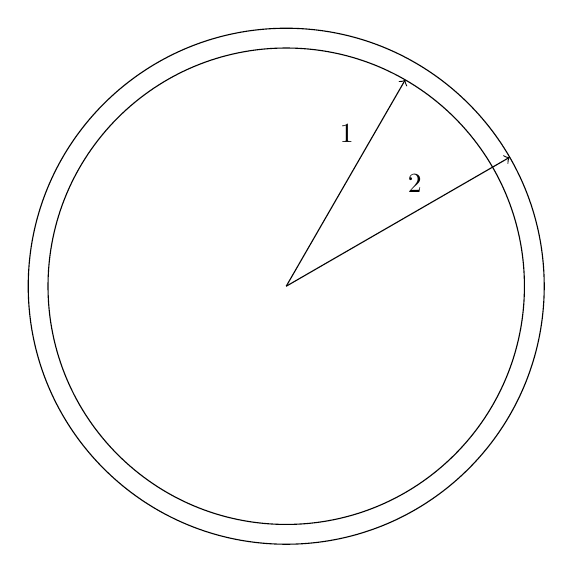
\begin{tikzpicture}[scale=6,auto]
        \draw (0,0) circle (0.50419);
      \draw[->] (0,0) -- node[pos=0.65] {1} (0.252,0.437);
      \draw (0,0) circle (0.5461);
      \draw[->] (0,0) -- node[pos=0.65] {2} (0.473,0.273);

      \end{tikzpicture}
      \begin{tikzpicture}
       \matrix [matrix of nodes]
      {
          Arrow & Radius (cm) & Material & \numrefheader \\
        1 & 0.50419 & \node[hyperlink node=mat_water]{Water}; & \ref{num:GTDPIRrad}\\ 
        2 & 0.54610 & \node[hyperlink node=mat_zirc]{Zircaloy}; & \ref{num:GTDPORrad}\\ 
      };
\end{tikzpicture}
\end{geoitem}

\begin{geoitem}{Instrument Tube Pin Geometry}{fig_instr_pin}\centering
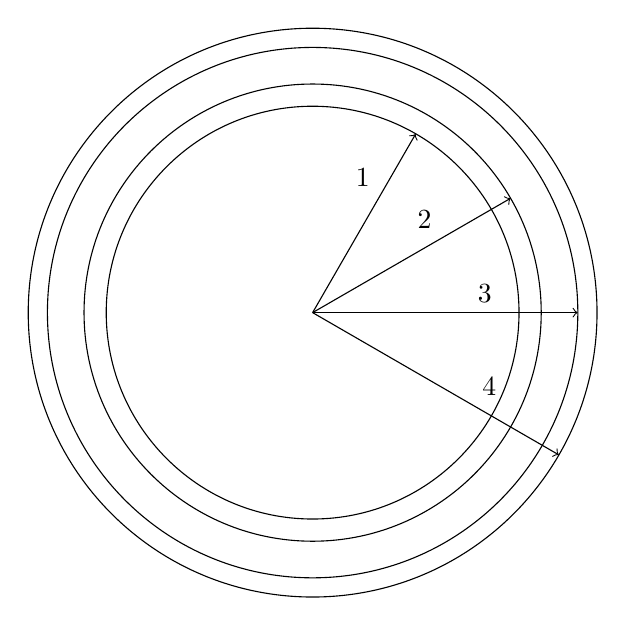
\begin{tikzpicture}[scale=6,auto]
        \draw (0,0) circle (0.43688);
      \draw[->] (0,0) -- node[pos=0.65] {1} (0.218,0.378);
      \draw (0,0) circle (0.48387);
      \draw[->] (0,0) -- node[pos=0.65] {2} (0.419,0.242);
      \draw (0,0) circle (0.56134);
      \draw[->] (0,0) -- node[pos=0.65] {3} (0.561,0.0);
      \draw (0,0) circle (0.60198);
      \draw[->] (0,0) -- node[pos=0.65] {4} (0.521,-0.301);

      \end{tikzpicture}
      \begin{tikzpicture}
       \matrix [matrix of nodes]
      {
          Arrow & Radius (cm) & Material & \numrefheader \\
        1 & 0.43688 & \node[hyperlink node=mat_air]{Air}; & \ref{num:ITthimIR}\\ 
        2 & 0.48387 & \node[hyperlink node=mat_zirc]{Zircaloy}; & \ref{num:ITthimOR}\\ 
        3 & 0.56134 & \node[hyperlink node=mat_water]{Water}; & \ref{num:GTIRrad}\\ 
        4 & 0.60198 & \node[hyperlink node=mat_zirc]{Zircaloy}; & \ref{num:GTORrad}\\ 
      };
\end{tikzpicture}
\\ \raggedright The thimble radii were chosen to be equivalent to the outer
thimble radii of control rods and burnable absorber rods by assumption. Note
that not all instrument tube positions contain the thimble defined by the first
2 radii in the diagram above, as discussed in Section \ref{sec:coreinstrpos}.
This pincell does not change at the dashpot.
\end{geoitem}

\begin{geoitem}{Bare Instrument Thimble Pin Geometry}{fig_instr_pin_bare}\centering
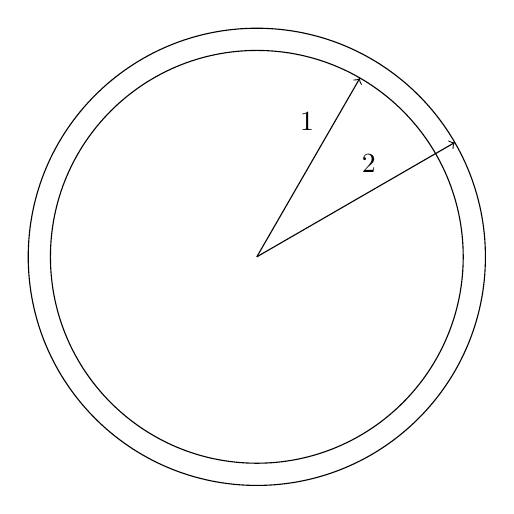
\begin{tikzpicture}[scale=6,auto]
        \draw (0,0) circle (0.43688);
      \draw[->] (0,0) -- node[pos=0.65] {1} (0.218,0.378);
      \draw (0,0) circle (0.48387);
      \draw[->] (0,0) -- node[pos=0.65] {2} (0.419,0.242);

      \end{tikzpicture}
      \begin{tikzpicture}
       \matrix [matrix of nodes]
      {
          Arrow & Radius (cm) & Material & \numrefheader \\
        1 & 0.43688 & \node[hyperlink node=mat_air]{Air}; & \ref{num:ITthimIR}\\ 
        2 & 0.48387 & \node[hyperlink node=mat_zirc]{Zircaloy}; & \ref{num:ITthimOR}\\ 
      };
\end{tikzpicture}
\\ \raggedright The bare instrument thimble for regions below the instrument tube.
\end{geoitem}

\begin{geoitem}{\acs{BP} Geometry above Dashpot}{fig_ba_pin}\centering
\input{specifications/pin/figs/tikz_ba}
\end{geoitem}
\begin{geoitem}{\acs{BP} Plenum Geometry}{fig_ba_pin_plenum}\centering
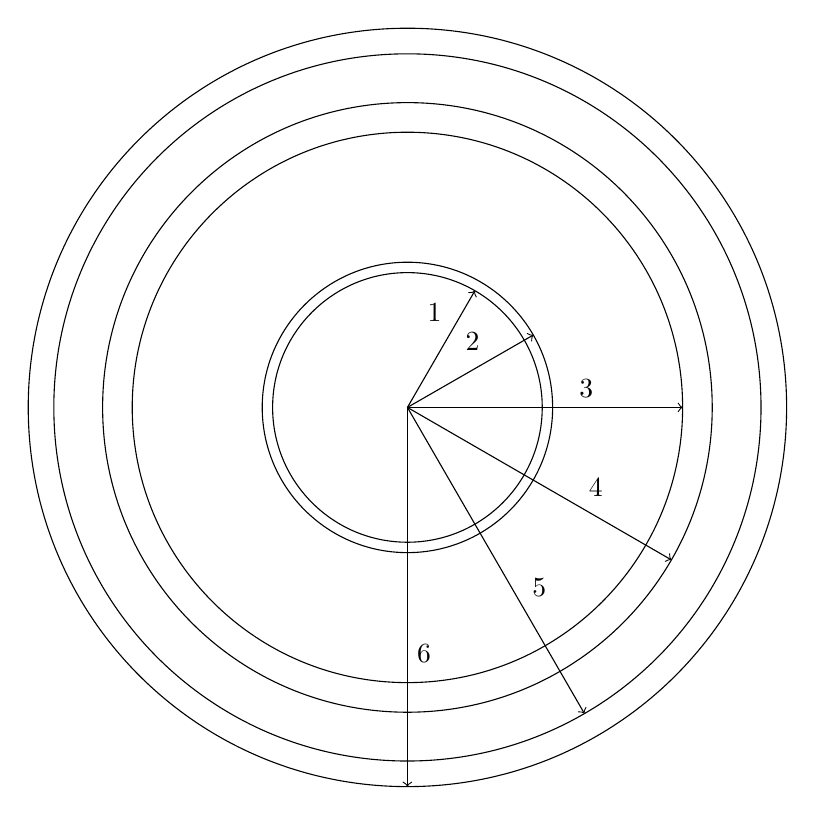
\begin{tikzpicture}[scale=8,auto]
        \draw (0,0) circle (0.214);
      \draw[->] (0,0) -- node[pos=0.65] {1} (0.107,0.185);
      \draw (0,0) circle (0.23051);
      \draw[->] (0,0) -- node[pos=0.65] {2} (0.2,0.115);
      \draw (0,0) circle (0.43688);
      \draw[->] (0,0) -- node[pos=0.65] {3} (0.437,0.0);
      \draw (0,0) circle (0.48387);
      \draw[->] (0,0) -- node[pos=0.65] {4} (0.419,-0.242);
      \draw (0,0) circle (0.56134);
      \draw[->] (0,0) -- node[pos=0.65] {5} (0.281,-0.486);
      \draw (0,0) circle (0.60198);
      \draw[->] (0,0) -- node[pos=0.65] {6} (0.0,-0.602);

      \end{tikzpicture}
      \begin{tikzpicture}
       \matrix [matrix of nodes]
      {
          Arrow & Radius (cm) & Material & \numrefheader \\
        1 & 0.21400 & \node[hyperlink node=mat_air]{Air}; & \ref{num:BPinnercladIR}\\ 
        2 & 0.23051 & \node[hyperlink node=mat_SS304]{SS304}; & \ref{num:BPinnercladOR}\\ 
        3 & 0.43688 & \node[hyperlink node=mat_helium]{Helium}; & \ref{num:BPoutercladIR}\\ 
        4 & 0.48387 & \node[hyperlink node=mat_SS304]{SS304}; & \ref{num:BPoutercladOR}\\ 
        5 & 0.56134 & \node[hyperlink node=mat_water]{Water}; & \ref{num:GTIRrad}\\ 
        6 & 0.60198 & \node[hyperlink node=mat_zirc]{Zircaloy}; & \ref{num:GTORrad}\\ 
      };
\end{tikzpicture}
\end{geoitem}

\begin{geoitem}{Control Rod Pin Upper Geometry}{fig_cr_pin_upper}\centering
\input{specifications/pin/figs/tikz_cr_upper}
\end{geoitem}
\begin{geoitem}{Control Rod Pin Lower Geometry}{fig_cr_pin}\centering
\input{specifications/pin/figs/tikz_cr}
\end{geoitem}
\begin{geoitem}{Control Rod Pin Spacer Geometry}{fig_cr_pin_spacer}\centering
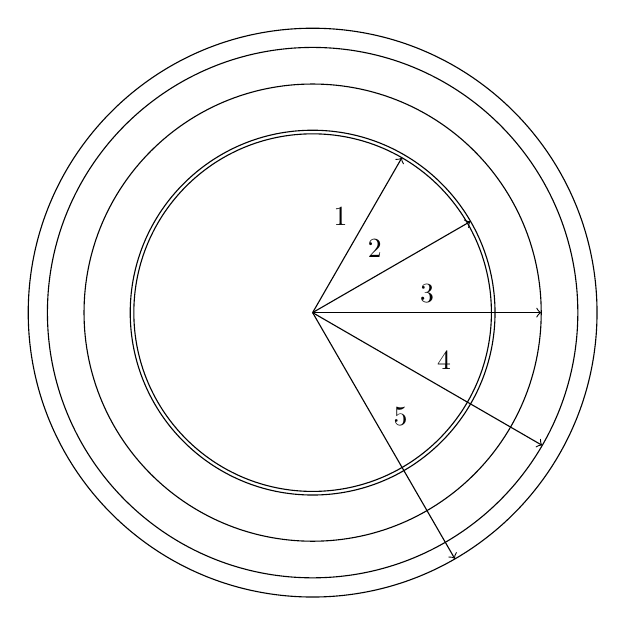
\begin{tikzpicture}[scale=6,auto]
        \draw (0,0) circle (0.37845);
      \draw[->] (0,0) -- node[pos=0.5] {1} (0.189,0.328);
      \draw (0,0) circle (0.38608);
      \draw[->] (0,0) -- node[pos=0.5] {2} (0.334,0.193);
      \draw (0,0) circle (0.48387);
      \draw[->] (0,0) -- node[pos=0.5] {3} (0.484,0.0);
      \draw (0,0) circle (0.56134);
      \draw[->] (0,0) -- node[pos=0.5] {4} (0.486,-0.281);
      \draw (0,0) circle (0.60198);
      \draw[->] (0,0) -- node[pos=0.5] {5} (0.301,-0.521);

      \end{tikzpicture}
      \begin{tikzpicture}
       \matrix [matrix of nodes]
      {
          Arrow & Radius (cm) & Material & \numrefheader \\
        1 & 0.37845 & \node[hyperlink node=mat_SS304]{SS304}; & \ref{num:CRspacerOR}\\ 
        2 & 0.38608 & \node[hyperlink node=mat_helium]{Helium}; & \ref{num:CRthimIR}\\ 
        3 & 0.48387 & \node[hyperlink node=mat_SS304]{SS304}; & \ref{num:CRthimOR}\\ 
        4 & 0.56134 & \node[hyperlink node=mat_water]{Water}; & \ref{num:GTIRrad}\\ 
        5 & 0.60198 & \node[hyperlink node=mat_zirc]{Zircaloy}; & \ref{num:GTORrad}\\ 
      };
\end{tikzpicture}
\end{geoitem}
\begin{geoitem}{Control Rod Pin Plenum Geometry}{fig_cr_pin_plenum}\centering
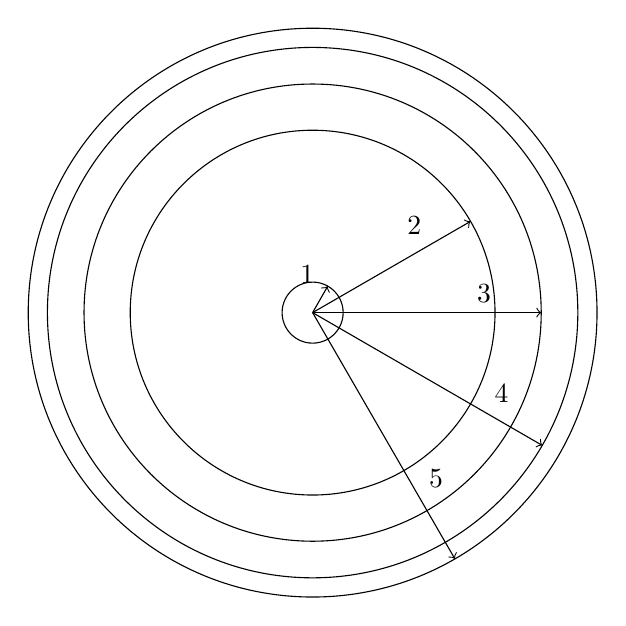
\begin{tikzpicture}[scale=6,auto]
        \draw (0,0) circle (0.06459);
      \draw[->] (0,0) -- node[pos=0.75] {1} (0.032,0.056);
      \draw (0,0) circle (0.38608);
      \draw[->] (0,0) -- node[pos=0.75] {2} (0.334,0.193);
      \draw (0,0) circle (0.48387);
      \draw[->] (0,0) -- node[pos=0.75] {3} (0.484,0.0);
      \draw (0,0) circle (0.56134);
      \draw[->] (0,0) -- node[pos=0.75] {4} (0.486,-0.281);
      \draw (0,0) circle (0.60198);
      \draw[->] (0,0) -- node[pos=0.75] {5} (0.301,-0.521);

      \end{tikzpicture}
      \begin{tikzpicture}
       \matrix [matrix of nodes]
      {
          Arrow & Radius (cm) & Material & \numrefheader \\
        1 & 0.06459 & \node[hyperlink node=mat_inconel]{Inconel}; & \ref{num:cr_plenum_spring}\\ 
        2 & 0.38608 & \node[hyperlink node=mat_helium]{Helium}; & \ref{num:CRthimIR}\\ 
        3 & 0.48387 & \node[hyperlink node=mat_SS304]{SS304}; & \ref{num:CRthimOR}\\ 
        4 & 0.56134 & \node[hyperlink node=mat_water]{Water}; & \ref{num:GTIRrad}\\ 
        5 & 0.60198 & \node[hyperlink node=mat_zirc]{Zircaloy}; & \ref{num:GTORrad}\\ 
      };
\end{tikzpicture}
\end{geoitem}


  \clearpage
\subsubsection[Fuel Assemblies]{Fuel Assemblies\texorpdfstring{\protect\sechypt{fuel_ass}{}}{}}

% some setup to make the assembly figures
% set assembly layout for tikz pictures

\newcommand{\Size}{0.7cm}% Adjust size of square as desired

\def\NumOfColumns{17}%
\def\Sequence{1/A, 2/B, 3/C, 4/D, 5/E, 6/F, 7/G, 8/H, 9/I, 10/J, 11/K, 12/L, 13/M, 14/N, 15/O, 16/P, 17/Q}% This needs to match \NumOfColumns 

\tikzset{Square/.style={
    inner sep=0pt,
    text width=\Size, 
    minimum size=\Size,
    draw=black,
%    fill=yellow!20,
    align=center
    }
}

\newcommand{\NodeAA}{$(1,1)$}%
\newcommand{\NodeAB}{$(1,2)$}%
\newcommand{\NodeAC}{$(1,3)$}%
\newcommand{\NodeAD}{$(1,4)$}%
\newcommand{\NodeAE}{$(1,5)$}%
\newcommand{\NodeAF}{$(1,6)$}%
\newcommand{\NodeAG}{$(1,7)$}%
\newcommand{\NodeAH}{$(1,8)$}%
\newcommand{\NodeAI}{$(1,9)$}%
\newcommand{\NodeAJ}{$(1,10)$}%
\newcommand{\NodeAK}{$(1,11)$}%
\newcommand{\NodeAL}{$(1,12)$}%
\newcommand{\NodeAM}{$(1,13)$}%
\newcommand{\NodeAN}{$(1,14)$}%
\newcommand{\NodeAO}{$(1,15)$}%
\newcommand{\NodeAP}{$(1,16)$}%
\newcommand{\NodeAQ}{$(1,17)$}%

\newcommand{\NodeBA}{$(2,1)$}%
\newcommand{\NodeBB}{$(2,2)$}%
\newcommand{\NodeBC}{$(2,3)$}%
\newcommand{\NodeBD}{$(2,4)$}%
\newcommand{\NodeBE}{$(2,5)$}%
\newcommand{\NodeBF}{$(2,6)$}%
\newcommand{\NodeBG}{$(2,7)$}%
\newcommand{\NodeBH}{$(2,8)$}%
\newcommand{\NodeBI}{$(2,9)$}%
\newcommand{\NodeBJ}{$(2,10)$}%
\newcommand{\NodeBK}{$(2,11)$}%
\newcommand{\NodeBL}{$(2,12)$}%
\newcommand{\NodeBM}{$(2,13)$}%
\newcommand{\NodeBN}{$(2,14)$}%
\newcommand{\NodeBO}{$(2,15)$}%
\newcommand{\NodeBP}{$(2,16)$}%
\newcommand{\NodeBQ}{$(2,17)$}%

\newcommand{\NodeCA}{$(3,1)$}%
\newcommand{\NodeCB}{$(3,2)$}%
\newcommand{\NodeCC}{$(3,3)$}%
\newcommand{\NodeCD}{$(3,4)$}%
\newcommand{\NodeCE}{$(3,5)$}%
\newcommand{\NodeCF}{$(3,6)$}%
\newcommand{\NodeCG}{$(3,7)$}%
\newcommand{\NodeCH}{$(3,8)$}%
\newcommand{\NodeCI}{$(3,9)$}%
\newcommand{\NodeCJ}{$(3,10)$}%
\newcommand{\NodeCK}{$(3,11)$}%
\newcommand{\NodeCL}{$(3,12)$}%
\newcommand{\NodeCM}{$(3,13)$}%
\newcommand{\NodeCN}{$(3,14)$}%
\newcommand{\NodeCO}{$(3,15)$}%
\newcommand{\NodeCP}{$(3,16)$}%
\newcommand{\NodeCQ}{$(3,17)$}%

\newcommand{\NodeDA}{$(4,1)$}%
\newcommand{\NodeDB}{$(4,2)$}%
\newcommand{\NodeDC}{$(4,3)$}%
\newcommand{\NodeDD}{$(4,4)$}%
\newcommand{\NodeDE}{$(4,5)$}%
\newcommand{\NodeDF}{$(4,6)$}%
\newcommand{\NodeDG}{$(4,7)$}%
\newcommand{\NodeDH}{$(4,8)$}%
\newcommand{\NodeDI}{$(4,9)$}%
\newcommand{\NodeDJ}{$(4,10)$}%
\newcommand{\NodeDK}{$(4,11)$}%
\newcommand{\NodeDL}{$(4,12)$}%
\newcommand{\NodeDM}{$(4,13)$}%
\newcommand{\NodeDN}{$(4,14)$}%
\newcommand{\NodeDO}{$(4,15)$}%
\newcommand{\NodeDP}{$(4,16)$}%
\newcommand{\NodeDQ}{$(4,17)$}%

\newcommand{\NodeEA}{$(5,1)$}%
\newcommand{\NodeEB}{$(5,2)$}%
\newcommand{\NodeEC}{$(5,3)$}%
\newcommand{\NodeED}{$(5,4)$}%
\newcommand{\NodeEE}{$(5,5)$}%
\newcommand{\NodeEF}{$(5,6)$}%
\newcommand{\NodeEG}{$(5,7)$}%
\newcommand{\NodeEH}{$(5,8)$}%
\newcommand{\NodeEI}{$(5,9)$}%
\newcommand{\NodeEJ}{$(5,10)$}%
\newcommand{\NodeEK}{$(5,11)$}%
\newcommand{\NodeEL}{$(5,12)$}%
\newcommand{\NodeEM}{$(5,13)$}%
\newcommand{\NodeEN}{$(5,14)$}%
\newcommand{\NodeEO}{$(5,15)$}%
\newcommand{\NodeEP}{$(5,16)$}%
\newcommand{\NodeEQ}{$(5,17)$}%

\newcommand{\NodeFA}{$(6,1)$}%
\newcommand{\NodeFB}{$(6,2)$}%
\newcommand{\NodeFC}{$(6,3)$}%
\newcommand{\NodeFD}{$(6,4)$}%
\newcommand{\NodeFE}{$(6,5)$}%
\newcommand{\NodeFF}{$(6,6)$}%
\newcommand{\NodeFG}{$(6,7)$}%
\newcommand{\NodeFH}{$(6,8)$}%
\newcommand{\NodeFI}{$(6,9)$}%
\newcommand{\NodeFJ}{$(6,10)$}%
\newcommand{\NodeFK}{$(6,11)$}%
\newcommand{\NodeFL}{$(6,12)$}%
\newcommand{\NodeFM}{$(6,13)$}%
\newcommand{\NodeFN}{$(6,14)$}%
\newcommand{\NodeFO}{$(6,15)$}%
\newcommand{\NodeFP}{$(6,16)$}%
\newcommand{\NodeFQ}{$(6,17)$}%

\newcommand{\NodeGA}{$(7,1)$}%
\newcommand{\NodeGB}{$(7,2)$}%
\newcommand{\NodeGC}{$(7,3)$}%
\newcommand{\NodeGD}{$(7,4)$}%
\newcommand{\NodeGE}{$(7,5)$}%
\newcommand{\NodeGF}{$(7,6)$}%
\newcommand{\NodeGG}{$(7,7)$}%
\newcommand{\NodeGH}{$(7,8)$}%
\newcommand{\NodeGI}{$(7,9)$}%
\newcommand{\NodeGJ}{$(7,10)$}%
\newcommand{\NodeGK}{$(7,11)$}%
\newcommand{\NodeGL}{$(7,12)$}%
\newcommand{\NodeGM}{$(7,13)$}%
\newcommand{\NodeGN}{$(7,14)$}%
\newcommand{\NodeGO}{$(7,15)$}%
\newcommand{\NodeGP}{$(7,16)$}%
\newcommand{\NodeGQ}{$(7,17)$}%

\newcommand{\NodeHA}{$(8,1)$}%
\newcommand{\NodeHB}{$(8,2)$}%
\newcommand{\NodeHC}{$(8,3)$}%
\newcommand{\NodeHD}{$(8,4)$}%
\newcommand{\NodeHE}{$(8,5)$}%
\newcommand{\NodeHF}{$(8,6)$}%
\newcommand{\NodeHG}{$(8,7)$}%
\newcommand{\NodeHH}{$(8,8)$}%
\newcommand{\NodeHI}{$(8,9)$}%
\newcommand{\NodeHJ}{$(8,10)$}%
\newcommand{\NodeHK}{$(8,11)$}%
\newcommand{\NodeHL}{$(8,12)$}%
\newcommand{\NodeHM}{$(8,13)$}%
\newcommand{\NodeHN}{$(8,14)$}%
\newcommand{\NodeHO}{$(8,15)$}%
\newcommand{\NodeHP}{$(8,16)$}%
\newcommand{\NodeHQ}{$(8,17)$}%

\newcommand{\NodeIA}{$(9,1)$}%
\newcommand{\NodeIB}{$(9,2)$}%
\newcommand{\NodeIC}{$(9,3)$}%
\newcommand{\NodeID}{$(9,4)$}%
\newcommand{\NodeIE}{$(9,5)$}%
\newcommand{\NodeIF}{$(9,6)$}%
\newcommand{\NodeIG}{$(9,7)$}%
\newcommand{\NodeIH}{$(9,8)$}%
\newcommand{\NodeII}{$(9,9)$}%
\newcommand{\NodeIJ}{$(9,10)$}%
\newcommand{\NodeIK}{$(9,11)$}%
\newcommand{\NodeIL}{$(9,12)$}%
\newcommand{\NodeIM}{$(9,13)$}%
\newcommand{\NodeIN}{$(9,14)$}%
\newcommand{\NodeIO}{$(9,15)$}%
\newcommand{\NodeIP}{$(9,16)$}%
\newcommand{\NodeIQ}{$(9,17)$}%

\newcommand{\NodeJA}{$(10,1)$}%
\newcommand{\NodeJB}{$(10,2)$}%
\newcommand{\NodeJC}{$(10,3)$}%
\newcommand{\NodeJD}{$(10,4)$}%
\newcommand{\NodeJE}{$(10,5)$}%
\newcommand{\NodeJF}{$(10,6)$}%
\newcommand{\NodeJG}{$(10,7)$}%
\newcommand{\NodeJH}{$(10,8)$}%
\newcommand{\NodeJI}{$(10,9)$}%
\newcommand{\NodeJJ}{$(10,10)$}%
\newcommand{\NodeJK}{$(10,11)$}%
\newcommand{\NodeJL}{$(10,12)$}%
\newcommand{\NodeJM}{$(10,13)$}%
\newcommand{\NodeJN}{$(10,14)$}%
\newcommand{\NodeJO}{$(10,15)$}%
\newcommand{\NodeJP}{$(10,16)$}%
\newcommand{\NodeJQ}{$(10,17)$}%

\newcommand{\NodeKA}{$(11,1)$}%
\newcommand{\NodeKB}{$(11,2)$}%
\newcommand{\NodeKC}{$(11,3)$}%
\newcommand{\NodeKD}{$(11,4)$}%
\newcommand{\NodeKE}{$(11,5)$}%
\newcommand{\NodeKF}{$(11,6)$}%
\newcommand{\NodeKG}{$(11,7)$}%
\newcommand{\NodeKH}{$(11,8)$}%
\newcommand{\NodeKI}{$(11,9)$}%
\newcommand{\NodeKJ}{$(11,10)$}%
\newcommand{\NodeKK}{$(11,11)$}%
\newcommand{\NodeKL}{$(11,12)$}%
\newcommand{\NodeKM}{$(11,13)$}%
\newcommand{\NodeKN}{$(11,14)$}%
\newcommand{\NodeKO}{$(11,15)$}%
\newcommand{\NodeKP}{$(11,16)$}%
\newcommand{\NodeKQ}{$(11,17)$}%

\newcommand{\NodeLA}{$(12,1)$}%
\newcommand{\NodeLB}{$(12,2)$}%
\newcommand{\NodeLC}{$(12,3)$}%
\newcommand{\NodeLD}{$(12,4)$}%
\newcommand{\NodeLE}{$(12,5)$}%
\newcommand{\NodeLF}{$(12,6)$}%
\newcommand{\NodeLG}{$(12,7)$}%
\newcommand{\NodeLH}{$(12,8)$}%
\newcommand{\NodeLI}{$(12,9)$}%
\newcommand{\NodeLJ}{$(12,10)$}%
\newcommand{\NodeLK}{$(12,11)$}%
\newcommand{\NodeLL}{$(12,12)$}%
\newcommand{\NodeLM}{$(12,13)$}%
\newcommand{\NodeLN}{$(12,14)$}%
\newcommand{\NodeLO}{$(12,15)$}%
\newcommand{\NodeLP}{$(12,16)$}%
\newcommand{\NodeLQ}{$(12,17)$}%

\newcommand{\NodeMA}{$(13,1)$}%
\newcommand{\NodeMB}{$(13,2)$}%
\newcommand{\NodeMC}{$(13,3)$}%
\newcommand{\NodeMD}{$(13,4)$}%
\newcommand{\NodeME}{$(13,5)$}%
\newcommand{\NodeMF}{$(13,6)$}%
\newcommand{\NodeMG}{$(13,7)$}%
\newcommand{\NodeMH}{$(13,8)$}%
\newcommand{\NodeMI}{$(13,9)$}%
\newcommand{\NodeMJ}{$(13,10)$}%
\newcommand{\NodeMK}{$(13,11)$}%
\newcommand{\NodeML}{$(13,12)$}%
\newcommand{\NodeMM}{$(13,13)$}%
\newcommand{\NodeMN}{$(13,14)$}%
\newcommand{\NodeMO}{$(13,15)$}%
\newcommand{\NodeMP}{$(13,16)$}%
\newcommand{\NodeMQ}{$(13,17)$}%

\newcommand{\NodeNA}{$(14,1)$}%
\newcommand{\NodeNB}{$(14,2)$}%
\newcommand{\NodeNC}{$(14,3)$}%
\newcommand{\NodeND}{$(14,4)$}%
\newcommand{\NodeNE}{$(14,5)$}%
\newcommand{\NodeNF}{$(14,6)$}%
\newcommand{\NodeNG}{$(14,7)$}%
\newcommand{\NodeNH}{$(14,8)$}%
\newcommand{\NodeNI}{$(14,9)$}%
\newcommand{\NodeNJ}{$(14,10)$}%
\newcommand{\NodeNK}{$(14,11)$}%
\newcommand{\NodeNL}{$(14,12)$}%
\newcommand{\NodeNM}{$(14,13)$}%
\newcommand{\NodeNN}{$(14,14)$}%
\newcommand{\NodeNO}{$(14,15)$}%
\newcommand{\NodeNP}{$(14,16)$}%
\newcommand{\NodeNQ}{$(14,17)$}%

\newcommand{\NodeOA}{$(15,1)$}%
\newcommand{\NodeOB}{$(15,2)$}%
\newcommand{\NodeOC}{$(15,3)$}%
\newcommand{\NodeOD}{$(15,4)$}%
\newcommand{\NodeOE}{$(15,5)$}%
\newcommand{\NodeOF}{$(15,6)$}%
\newcommand{\NodeOG}{$(15,7)$}%
\newcommand{\NodeOH}{$(15,8)$}%
\newcommand{\NodeOI}{$(15,9)$}%
\newcommand{\NodeOJ}{$(15,10)$}%
\newcommand{\NodeOK}{$(15,11)$}%
\newcommand{\NodeOL}{$(15,12)$}%
\newcommand{\NodeOM}{$(15,13)$}%
\newcommand{\NodeON}{$(15,14)$}%
\newcommand{\NodeOO}{$(15,15)$}%
\newcommand{\NodeOP}{$(15,16)$}%
\newcommand{\NodeOQ}{$(15,17)$}%

\newcommand{\NodePA}{$(16,1)$}%
\newcommand{\NodePB}{$(16,2)$}%
\newcommand{\NodePC}{$(16,3)$}%
\newcommand{\NodePD}{$(16,4)$}%
\newcommand{\NodePE}{$(16,5)$}%
\newcommand{\NodePF}{$(16,6)$}%
\newcommand{\NodePG}{$(16,7)$}%
\newcommand{\NodePH}{$(16,8)$}%
\newcommand{\NodePI}{$(16,9)$}%
\newcommand{\NodePJ}{$(16,10)$}%
\newcommand{\NodePK}{$(16,11)$}%
\newcommand{\NodePL}{$(16,12)$}%
\newcommand{\NodePM}{$(16,13)$}%
\newcommand{\NodePN}{$(16,14)$}%
\newcommand{\NodePO}{$(16,15)$}%
\newcommand{\NodePP}{$(16,16)$}%
\newcommand{\NodePQ}{$(16,17)$}%

\newcommand{\NodeQA}{$(17,1)$}%
\newcommand{\NodeQB}{$(17,2)$}%
\newcommand{\NodeQC}{$(17,3)$}%
\newcommand{\NodeQD}{$(17,4)$}%
\newcommand{\NodeQE}{$(17,5)$}%
\newcommand{\NodeQF}{$(17,6)$}%
\newcommand{\NodeQG}{$(17,7)$}%
\newcommand{\NodeQH}{$(17,8)$}%
\newcommand{\NodeQI}{$(17,9)$}%
\newcommand{\NodeQJ}{$(17,10)$}%
\newcommand{\NodeQK}{$(17,11)$}%
\newcommand{\NodeQL}{$(17,12)$}%
\newcommand{\NodeQM}{$(17,13)$}%
\newcommand{\NodeQN}{$(17,14)$}%
\newcommand{\NodeQO}{$(17,15)$}%
\newcommand{\NodeQP}{$(17,16)$}%
\newcommand{\NodeQQ}{$(17,17)$}%

\newcommand{\NodeLinkAA}{}
\newcommand{\NodeLinkAB}{}
\newcommand{\NodeLinkAC}{}
\newcommand{\NodeLinkAD}{}
\newcommand{\NodeLinkAE}{}
\newcommand{\NodeLinkAF}{}
\newcommand{\NodeLinkAG}{}
\newcommand{\NodeLinkAH}{}
\newcommand{\NodeLinkAI}{}
\newcommand{\NodeLinkAJ}{}
\newcommand{\NodeLinkAK}{}
\newcommand{\NodeLinkAL}{}
\newcommand{\NodeLinkAM}{}
\newcommand{\NodeLinkAN}{}
\newcommand{\NodeLinkAO}{}
\newcommand{\NodeLinkAP}{}
\newcommand{\NodeLinkAQ}{}

\newcommand{\NodeLinkBA}{}
\newcommand{\NodeLinkBB}{}
\newcommand{\NodeLinkBC}{}
\newcommand{\NodeLinkBD}{}
\newcommand{\NodeLinkBE}{}
\newcommand{\NodeLinkBF}{}
\newcommand{\NodeLinkBG}{}
\newcommand{\NodeLinkBH}{}
\newcommand{\NodeLinkBI}{}
\newcommand{\NodeLinkBJ}{}
\newcommand{\NodeLinkBK}{}
\newcommand{\NodeLinkBL}{}
\newcommand{\NodeLinkBM}{}
\newcommand{\NodeLinkBN}{}
\newcommand{\NodeLinkBO}{}
\newcommand{\NodeLinkBP}{}
\newcommand{\NodeLinkBQ}{}

\newcommand{\NodeLinkCA}{}
\newcommand{\NodeLinkCB}{}
\newcommand{\NodeLinkCC}{}
\newcommand{\NodeLinkCD}{}
\newcommand{\NodeLinkCE}{}
\newcommand{\NodeLinkCF}{}
\newcommand{\NodeLinkCG}{}
\newcommand{\NodeLinkCH}{}
\newcommand{\NodeLinkCI}{}
\newcommand{\NodeLinkCJ}{}
\newcommand{\NodeLinkCK}{}
\newcommand{\NodeLinkCL}{}
\newcommand{\NodeLinkCM}{}
\newcommand{\NodeLinkCN}{}
\newcommand{\NodeLinkCO}{}
\newcommand{\NodeLinkCP}{}
\newcommand{\NodeLinkCQ}{}

\newcommand{\NodeLinkDA}{}
\newcommand{\NodeLinkDB}{}
\newcommand{\NodeLinkDC}{}
\newcommand{\NodeLinkDD}{}
\newcommand{\NodeLinkDE}{}
\newcommand{\NodeLinkDF}{}
\newcommand{\NodeLinkDG}{}
\newcommand{\NodeLinkDH}{}
\newcommand{\NodeLinkDI}{}
\newcommand{\NodeLinkDJ}{}
\newcommand{\NodeLinkDK}{}
\newcommand{\NodeLinkDL}{}
\newcommand{\NodeLinkDM}{}
\newcommand{\NodeLinkDN}{}
\newcommand{\NodeLinkDO}{}
\newcommand{\NodeLinkDP}{}
\newcommand{\NodeLinkDQ}{}

\newcommand{\NodeLinkEA}{}
\newcommand{\NodeLinkEB}{}
\newcommand{\NodeLinkEC}{}
\newcommand{\NodeLinkED}{}
\newcommand{\NodeLinkEE}{}
\newcommand{\NodeLinkEF}{}
\newcommand{\NodeLinkEG}{}
\newcommand{\NodeLinkEH}{}
\newcommand{\NodeLinkEI}{}
\newcommand{\NodeLinkEJ}{}
\newcommand{\NodeLinkEK}{}
\newcommand{\NodeLinkEL}{}
\newcommand{\NodeLinkEM}{}
\newcommand{\NodeLinkEN}{}
\newcommand{\NodeLinkEO}{}
\newcommand{\NodeLinkEP}{}
\newcommand{\NodeLinkEQ}{}

\newcommand{\NodeLinkFA}{}
\newcommand{\NodeLinkFB}{}
\newcommand{\NodeLinkFC}{}
\newcommand{\NodeLinkFD}{}
\newcommand{\NodeLinkFE}{}
\newcommand{\NodeLinkFF}{}
\newcommand{\NodeLinkFG}{}
\newcommand{\NodeLinkFH}{}
\newcommand{\NodeLinkFI}{}
\newcommand{\NodeLinkFJ}{}
\newcommand{\NodeLinkFK}{}
\newcommand{\NodeLinkFL}{}
\newcommand{\NodeLinkFM}{}
\newcommand{\NodeLinkFN}{}
\newcommand{\NodeLinkFO}{}
\newcommand{\NodeLinkFP}{}
\newcommand{\NodeLinkFQ}{}

\newcommand{\NodeLinkGA}{}
\newcommand{\NodeLinkGB}{}
\newcommand{\NodeLinkGC}{}
\newcommand{\NodeLinkGD}{}
\newcommand{\NodeLinkGE}{}
\newcommand{\NodeLinkGF}{}
\newcommand{\NodeLinkGG}{}
\newcommand{\NodeLinkGH}{}
\newcommand{\NodeLinkGI}{}
\newcommand{\NodeLinkGJ}{}
\newcommand{\NodeLinkGK}{}
\newcommand{\NodeLinkGL}{}
\newcommand{\NodeLinkGM}{}
\newcommand{\NodeLinkGN}{}
\newcommand{\NodeLinkGO}{}
\newcommand{\NodeLinkGP}{}
\newcommand{\NodeLinkGQ}{}

\newcommand{\NodeLinkHA}{}
\newcommand{\NodeLinkHB}{}
\newcommand{\NodeLinkHC}{}
\newcommand{\NodeLinkHD}{}
\newcommand{\NodeLinkHE}{}
\newcommand{\NodeLinkHF}{}
\newcommand{\NodeLinkHG}{}
\newcommand{\NodeLinkHH}{}
\newcommand{\NodeLinkHI}{}
\newcommand{\NodeLinkHJ}{}
\newcommand{\NodeLinkHK}{}
\newcommand{\NodeLinkHL}{}
\newcommand{\NodeLinkHM}{}
\newcommand{\NodeLinkHN}{}
\newcommand{\NodeLinkHO}{}
\newcommand{\NodeLinkHP}{}
\newcommand{\NodeLinkHQ}{}

\newcommand{\NodeLinkIA}{}
\newcommand{\NodeLinkIB}{}
\newcommand{\NodeLinkIC}{}
\newcommand{\NodeLinkID}{}
\newcommand{\NodeLinkIE}{}
\newcommand{\NodeLinkIF}{}
\newcommand{\NodeLinkIG}{}
\newcommand{\NodeLinkIH}{}
\newcommand{\NodeLinkII}{}
\newcommand{\NodeLinkIJ}{}
\newcommand{\NodeLinkIK}{}
\newcommand{\NodeLinkIL}{}
\newcommand{\NodeLinkIM}{}
\newcommand{\NodeLinkIN}{}
\newcommand{\NodeLinkIO}{}
\newcommand{\NodeLinkIP}{}
\newcommand{\NodeLinkIQ}{}

\newcommand{\NodeLinkJA}{}
\newcommand{\NodeLinkJB}{}
\newcommand{\NodeLinkJC}{}
\newcommand{\NodeLinkJD}{}
\newcommand{\NodeLinkJE}{}
\newcommand{\NodeLinkJF}{}
\newcommand{\NodeLinkJG}{}
\newcommand{\NodeLinkJH}{}
\newcommand{\NodeLinkJI}{}
\newcommand{\NodeLinkJJ}{}
\newcommand{\NodeLinkJK}{}
\newcommand{\NodeLinkJL}{}
\newcommand{\NodeLinkJM}{}
\newcommand{\NodeLinkJN}{}
\newcommand{\NodeLinkJO}{}
\newcommand{\NodeLinkJP}{}
\newcommand{\NodeLinkJQ}{}

\newcommand{\NodeLinkKA}{}
\newcommand{\NodeLinkKB}{}
\newcommand{\NodeLinkKC}{}
\newcommand{\NodeLinkKD}{}
\newcommand{\NodeLinkKE}{}
\newcommand{\NodeLinkKF}{}
\newcommand{\NodeLinkKG}{}
\newcommand{\NodeLinkKH}{}
\newcommand{\NodeLinkKI}{}
\newcommand{\NodeLinkKJ}{}
\newcommand{\NodeLinkKK}{}
\newcommand{\NodeLinkKL}{}
\newcommand{\NodeLinkKM}{}
\newcommand{\NodeLinkKN}{}
\newcommand{\NodeLinkKO}{}
\newcommand{\NodeLinkKP}{}
\newcommand{\NodeLinkKQ}{}

\newcommand{\NodeLinkLA}{}
\newcommand{\NodeLinkLB}{}
\newcommand{\NodeLinkLC}{}
\newcommand{\NodeLinkLD}{}
\newcommand{\NodeLinkLE}{}
\newcommand{\NodeLinkLF}{}
\newcommand{\NodeLinkLG}{}
\newcommand{\NodeLinkLH}{}
\newcommand{\NodeLinkLI}{}
\newcommand{\NodeLinkLJ}{}
\newcommand{\NodeLinkLK}{}
\newcommand{\NodeLinkLL}{}
\newcommand{\NodeLinkLM}{}
\newcommand{\NodeLinkLN}{}
\newcommand{\NodeLinkLO}{}
\newcommand{\NodeLinkLP}{}
\newcommand{\NodeLinkLQ}{}

\newcommand{\NodeLinkMA}{}
\newcommand{\NodeLinkMB}{}
\newcommand{\NodeLinkMC}{}
\newcommand{\NodeLinkMD}{}
\newcommand{\NodeLinkME}{}
\newcommand{\NodeLinkMF}{}
\newcommand{\NodeLinkMG}{}
\newcommand{\NodeLinkMH}{}
\newcommand{\NodeLinkMI}{}
\newcommand{\NodeLinkMJ}{}
\newcommand{\NodeLinkMK}{}
\newcommand{\NodeLinkML}{}
\newcommand{\NodeLinkMM}{}
\newcommand{\NodeLinkMN}{}
\newcommand{\NodeLinkMO}{}
\newcommand{\NodeLinkMP}{}
\newcommand{\NodeLinkMQ}{}

\newcommand{\NodeLinkNA}{}
\newcommand{\NodeLinkNB}{}
\newcommand{\NodeLinkNC}{}
\newcommand{\NodeLinkND}{}
\newcommand{\NodeLinkNE}{}
\newcommand{\NodeLinkNF}{}
\newcommand{\NodeLinkNG}{}
\newcommand{\NodeLinkNH}{}
\newcommand{\NodeLinkNI}{}
\newcommand{\NodeLinkNJ}{}
\newcommand{\NodeLinkNK}{}
\newcommand{\NodeLinkNL}{}
\newcommand{\NodeLinkNM}{}
\newcommand{\NodeLinkNN}{}
\newcommand{\NodeLinkNO}{}
\newcommand{\NodeLinkNP}{}
\newcommand{\NodeLinkNQ}{}

\newcommand{\NodeLinkOA}{}
\newcommand{\NodeLinkOB}{}
\newcommand{\NodeLinkOC}{}
\newcommand{\NodeLinkOD}{}
\newcommand{\NodeLinkOE}{}
\newcommand{\NodeLinkOF}{}
\newcommand{\NodeLinkOG}{}
\newcommand{\NodeLinkOH}{}
\newcommand{\NodeLinkOI}{}
\newcommand{\NodeLinkOJ}{}
\newcommand{\NodeLinkOK}{}
\newcommand{\NodeLinkOL}{}
\newcommand{\NodeLinkOM}{}
\newcommand{\NodeLinkON}{}
\newcommand{\NodeLinkOO}{}
\newcommand{\NodeLinkOP}{}
\newcommand{\NodeLinkOQ}{}

\newcommand{\NodeLinkPA}{}
\newcommand{\NodeLinkPB}{}
\newcommand{\NodeLinkPC}{}
\newcommand{\NodeLinkPD}{}
\newcommand{\NodeLinkPE}{}
\newcommand{\NodeLinkPF}{}
\newcommand{\NodeLinkPG}{}
\newcommand{\NodeLinkPH}{}
\newcommand{\NodeLinkPI}{}
\newcommand{\NodeLinkPJ}{}
\newcommand{\NodeLinkPK}{}
\newcommand{\NodeLinkPL}{}
\newcommand{\NodeLinkPM}{}
\newcommand{\NodeLinkPN}{}
\newcommand{\NodeLinkPO}{}
\newcommand{\NodeLinkPP}{}
\newcommand{\NodeLinkPQ}{}

\newcommand{\NodeLinkQA}{}
\newcommand{\NodeLinkQB}{}
\newcommand{\NodeLinkQC}{}
\newcommand{\NodeLinkQD}{}
\newcommand{\NodeLinkQE}{}
\newcommand{\NodeLinkQF}{}
\newcommand{\NodeLinkQG}{}
\newcommand{\NodeLinkQH}{}
\newcommand{\NodeLinkQI}{}
\newcommand{\NodeLinkQJ}{}
\newcommand{\NodeLinkQK}{}
\newcommand{\NodeLinkQL}{}
\newcommand{\NodeLinkQM}{}
\newcommand{\NodeLinkQN}{}
\newcommand{\NodeLinkQO}{}
\newcommand{\NodeLinkQP}{}
\newcommand{\NodeLinkQQ}{}



\newcommand{\NodeFillAA}{}
\newcommand{\NodeFillAB}{}
\newcommand{\NodeFillAC}{}
\newcommand{\NodeFillAD}{}
\newcommand{\NodeFillAE}{}
\newcommand{\NodeFillAF}{}
\newcommand{\NodeFillAG}{}
\newcommand{\NodeFillAH}{}
\newcommand{\NodeFillAI}{}
\newcommand{\NodeFillAJ}{}
\newcommand{\NodeFillAK}{}
\newcommand{\NodeFillAL}{}
\newcommand{\NodeFillAM}{}
\newcommand{\NodeFillAN}{}
\newcommand{\NodeFillAO}{}
\newcommand{\NodeFillAP}{}
\newcommand{\NodeFillAQ}{}

\newcommand{\NodeFillBA}{}
\newcommand{\NodeFillBB}{}
\newcommand{\NodeFillBC}{}
\newcommand{\NodeFillBD}{}
\newcommand{\NodeFillBE}{}
\newcommand{\NodeFillBF}{}
\newcommand{\NodeFillBG}{}
\newcommand{\NodeFillBH}{}
\newcommand{\NodeFillBI}{}
\newcommand{\NodeFillBJ}{}
\newcommand{\NodeFillBK}{}
\newcommand{\NodeFillBL}{}
\newcommand{\NodeFillBM}{}
\newcommand{\NodeFillBN}{}
\newcommand{\NodeFillBO}{}
\newcommand{\NodeFillBP}{}
\newcommand{\NodeFillBQ}{}

\newcommand{\NodeFillCA}{}
\newcommand{\NodeFillCB}{}
\newcommand{\NodeFillCC}{}
\newcommand{\NodeFillCD}{}
\newcommand{\NodeFillCE}{}
\newcommand{\NodeFillCF}{}
\newcommand{\NodeFillCG}{}
\newcommand{\NodeFillCH}{}
\newcommand{\NodeFillCI}{}
\newcommand{\NodeFillCJ}{}
\newcommand{\NodeFillCK}{}
\newcommand{\NodeFillCL}{}
\newcommand{\NodeFillCM}{}
\newcommand{\NodeFillCN}{}
\newcommand{\NodeFillCO}{}
\newcommand{\NodeFillCP}{}
\newcommand{\NodeFillCQ}{}

\newcommand{\NodeFillDA}{}
\newcommand{\NodeFillDB}{}
\newcommand{\NodeFillDC}{}
\newcommand{\NodeFillDD}{}
\newcommand{\NodeFillDE}{}
\newcommand{\NodeFillDF}{}
\newcommand{\NodeFillDG}{}
\newcommand{\NodeFillDH}{}
\newcommand{\NodeFillDI}{}
\newcommand{\NodeFillDJ}{}
\newcommand{\NodeFillDK}{}
\newcommand{\NodeFillDL}{}
\newcommand{\NodeFillDM}{}
\newcommand{\NodeFillDN}{}
\newcommand{\NodeFillDO}{}
\newcommand{\NodeFillDP}{}
\newcommand{\NodeFillDQ}{}

\newcommand{\NodeFillEA}{}
\newcommand{\NodeFillEB}{}
\newcommand{\NodeFillEC}{}
\newcommand{\NodeFillED}{}
\newcommand{\NodeFillEE}{}
\newcommand{\NodeFillEF}{}
\newcommand{\NodeFillEG}{}
\newcommand{\NodeFillEH}{}
\newcommand{\NodeFillEI}{}
\newcommand{\NodeFillEJ}{}
\newcommand{\NodeFillEK}{}
\newcommand{\NodeFillEL}{}
\newcommand{\NodeFillEM}{}
\newcommand{\NodeFillEN}{}
\newcommand{\NodeFillEO}{}
\newcommand{\NodeFillEP}{}
\newcommand{\NodeFillEQ}{}

\newcommand{\NodeFillFA}{}
\newcommand{\NodeFillFB}{}
\newcommand{\NodeFillFC}{}
\newcommand{\NodeFillFD}{}
\newcommand{\NodeFillFE}{}
\newcommand{\NodeFillFF}{}
\newcommand{\NodeFillFG}{}
\newcommand{\NodeFillFH}{}
\newcommand{\NodeFillFI}{}
\newcommand{\NodeFillFJ}{}
\newcommand{\NodeFillFK}{}
\newcommand{\NodeFillFL}{}
\newcommand{\NodeFillFM}{}
\newcommand{\NodeFillFN}{}
\newcommand{\NodeFillFO}{}
\newcommand{\NodeFillFP}{}
\newcommand{\NodeFillFQ}{}

\newcommand{\NodeFillGA}{}
\newcommand{\NodeFillGB}{}
\newcommand{\NodeFillGC}{}
\newcommand{\NodeFillGD}{}
\newcommand{\NodeFillGE}{}
\newcommand{\NodeFillGF}{}
\newcommand{\NodeFillGG}{}
\newcommand{\NodeFillGH}{}
\newcommand{\NodeFillGI}{}
\newcommand{\NodeFillGJ}{}
\newcommand{\NodeFillGK}{}
\newcommand{\NodeFillGL}{}
\newcommand{\NodeFillGM}{}
\newcommand{\NodeFillGN}{}
\newcommand{\NodeFillGO}{}
\newcommand{\NodeFillGP}{}
\newcommand{\NodeFillGQ}{}

\newcommand{\NodeFillHA}{}
\newcommand{\NodeFillHB}{}
\newcommand{\NodeFillHC}{}
\newcommand{\NodeFillHD}{}
\newcommand{\NodeFillHE}{}
\newcommand{\NodeFillHF}{}
\newcommand{\NodeFillHG}{}
\newcommand{\NodeFillHH}{}
\newcommand{\NodeFillHI}{}
\newcommand{\NodeFillHJ}{}
\newcommand{\NodeFillHK}{}
\newcommand{\NodeFillHL}{}
\newcommand{\NodeFillHM}{}
\newcommand{\NodeFillHN}{}
\newcommand{\NodeFillHO}{}
\newcommand{\NodeFillHP}{}
\newcommand{\NodeFillHQ}{}

\newcommand{\NodeFillIA}{}
\newcommand{\NodeFillIB}{}
\newcommand{\NodeFillIC}{}
\newcommand{\NodeFillID}{}
\newcommand{\NodeFillIE}{}
\newcommand{\NodeFillIF}{}
\newcommand{\NodeFillIG}{}
\newcommand{\NodeFillIH}{}
\newcommand{\NodeFillII}{}
\newcommand{\NodeFillIJ}{}
\newcommand{\NodeFillIK}{}
\newcommand{\NodeFillIL}{}
\newcommand{\NodeFillIM}{}
\newcommand{\NodeFillIN}{}
\newcommand{\NodeFillIO}{}
\newcommand{\NodeFillIP}{}
\newcommand{\NodeFillIQ}{}

\newcommand{\NodeFillJA}{}
\newcommand{\NodeFillJB}{}
\newcommand{\NodeFillJC}{}
\newcommand{\NodeFillJD}{}
\newcommand{\NodeFillJE}{}
\newcommand{\NodeFillJF}{}
\newcommand{\NodeFillJG}{}
\newcommand{\NodeFillJH}{}
\newcommand{\NodeFillJI}{}
\newcommand{\NodeFillJJ}{}
\newcommand{\NodeFillJK}{}
\newcommand{\NodeFillJL}{}
\newcommand{\NodeFillJM}{}
\newcommand{\NodeFillJN}{}
\newcommand{\NodeFillJO}{}
\newcommand{\NodeFillJP}{}
\newcommand{\NodeFillJQ}{}

\newcommand{\NodeFillKA}{}
\newcommand{\NodeFillKB}{}
\newcommand{\NodeFillKC}{}
\newcommand{\NodeFillKD}{}
\newcommand{\NodeFillKE}{}
\newcommand{\NodeFillKF}{}
\newcommand{\NodeFillKG}{}
\newcommand{\NodeFillKH}{}
\newcommand{\NodeFillKI}{}
\newcommand{\NodeFillKJ}{}
\newcommand{\NodeFillKK}{}
\newcommand{\NodeFillKL}{}
\newcommand{\NodeFillKM}{}
\newcommand{\NodeFillKN}{}
\newcommand{\NodeFillKO}{}
\newcommand{\NodeFillKP}{}
\newcommand{\NodeFillKQ}{}

\newcommand{\NodeFillLA}{}
\newcommand{\NodeFillLB}{}
\newcommand{\NodeFillLC}{}
\newcommand{\NodeFillLD}{}
\newcommand{\NodeFillLE}{}
\newcommand{\NodeFillLF}{}
\newcommand{\NodeFillLG}{}
\newcommand{\NodeFillLH}{}
\newcommand{\NodeFillLI}{}
\newcommand{\NodeFillLJ}{}
\newcommand{\NodeFillLK}{}
\newcommand{\NodeFillLL}{}
\newcommand{\NodeFillLM}{}
\newcommand{\NodeFillLN}{}
\newcommand{\NodeFillLO}{}
\newcommand{\NodeFillLP}{}
\newcommand{\NodeFillLQ}{}

\newcommand{\NodeFillMA}{}
\newcommand{\NodeFillMB}{}
\newcommand{\NodeFillMC}{}
\newcommand{\NodeFillMD}{}
\newcommand{\NodeFillME}{}
\newcommand{\NodeFillMF}{}
\newcommand{\NodeFillMG}{}
\newcommand{\NodeFillMH}{}
\newcommand{\NodeFillMI}{}
\newcommand{\NodeFillMJ}{}
\newcommand{\NodeFillMK}{}
\newcommand{\NodeFillML}{}
\newcommand{\NodeFillMM}{}
\newcommand{\NodeFillMN}{}
\newcommand{\NodeFillMO}{}
\newcommand{\NodeFillMP}{}
\newcommand{\NodeFillMQ}{}

\newcommand{\NodeFillNA}{}
\newcommand{\NodeFillNB}{}
\newcommand{\NodeFillNC}{}
\newcommand{\NodeFillND}{}
\newcommand{\NodeFillNE}{}
\newcommand{\NodeFillNF}{}
\newcommand{\NodeFillNG}{}
\newcommand{\NodeFillNH}{}
\newcommand{\NodeFillNI}{}
\newcommand{\NodeFillNJ}{}
\newcommand{\NodeFillNK}{}
\newcommand{\NodeFillNL}{}
\newcommand{\NodeFillNM}{}
\newcommand{\NodeFillNN}{}
\newcommand{\NodeFillNO}{}
\newcommand{\NodeFillNP}{}
\newcommand{\NodeFillNQ}{}

\newcommand{\NodeFillOA}{}
\newcommand{\NodeFillOB}{}
\newcommand{\NodeFillOC}{}
\newcommand{\NodeFillOD}{}
\newcommand{\NodeFillOE}{}
\newcommand{\NodeFillOF}{}
\newcommand{\NodeFillOG}{}
\newcommand{\NodeFillOH}{}
\newcommand{\NodeFillOI}{}
\newcommand{\NodeFillOJ}{}
\newcommand{\NodeFillOK}{}
\newcommand{\NodeFillOL}{}
\newcommand{\NodeFillOM}{}
\newcommand{\NodeFillON}{}
\newcommand{\NodeFillOO}{}
\newcommand{\NodeFillOP}{}
\newcommand{\NodeFillOQ}{}

\newcommand{\NodeFillPA}{}
\newcommand{\NodeFillPB}{}
\newcommand{\NodeFillPC}{}
\newcommand{\NodeFillPD}{}
\newcommand{\NodeFillPE}{}
\newcommand{\NodeFillPF}{}
\newcommand{\NodeFillPG}{}
\newcommand{\NodeFillPH}{}
\newcommand{\NodeFillPI}{}
\newcommand{\NodeFillPJ}{}
\newcommand{\NodeFillPK}{}
\newcommand{\NodeFillPL}{}
\newcommand{\NodeFillPM}{}
\newcommand{\NodeFillPN}{}
\newcommand{\NodeFillPO}{}
\newcommand{\NodeFillPP}{}
\newcommand{\NodeFillPQ}{}

\newcommand{\NodeFillQA}{}
\newcommand{\NodeFillQB}{}
\newcommand{\NodeFillQC}{}
\newcommand{\NodeFillQD}{}
\newcommand{\NodeFillQE}{}
\newcommand{\NodeFillQF}{}
\newcommand{\NodeFillQG}{}
\newcommand{\NodeFillQH}{}
\newcommand{\NodeFillQI}{}
\newcommand{\NodeFillQJ}{}
\newcommand{\NodeFillQK}{}
\newcommand{\NodeFillQL}{}
\newcommand{\NodeFillQM}{}
\newcommand{\NodeFillQN}{}
\newcommand{\NodeFillQO}{}
\newcommand{\NodeFillQP}{}
\newcommand{\NodeFillQQ}{}




Each of the assemblies in the core is made up of a $17\times17$ array of pins
described in Section \ref{sec:pintypes}. Table \ref{table_assembly_overview}
outlines the important parameters of each, and the positions of the guide tubes
are shown in Figure \ref{ass_base}.

Assemblies are made up of one of three different enrichment fuel pins, and the
guide tube positions can be filled with one of several different burnable
absorber configurations described in Section \ref{sec:ba_configs}. For any
configuration, the center guide tube may contain an instrument tube. The details
of the layout of these features throughout the core are described in Section
\ref{sec:corespec}.

\begin{table}[htpb]
  
  \caption{Fuel assembly parameters. \label{table_assembly_overview}}
  
  \begin{tabularx}{\textwidth}{l C c}

    \toprule
    & & Source\\
    \midrule
    \midrule
    Fuel Assembly Lattice Pitch & 21.50364 cm & \ref{num:ass_pitch}\\
    Pin Lattice Pitch & 1.25984 cm & \ref{num:pin_pitch}\\
    Pin Lattice Configuration & $17 \times 17$ & \ref{num:fuellattice}\\
    No. Fuel Rods & 264 & \ref{num:fuellattice}\\
    No. Guide Tube Positions & 24 & \ref{num:fuellattice}\\
    No. Instrument Tube Positions & 1 & \ref{num:fuellattice}\\
    \\
    No. Grid Spacers & 8 & \ref{num:fuellattice}\\
    Top/Bottom Grid Spacer Material & \hyperref[mat_inconel]{Inconel 718} & \ref{num:fuellattice} \\
    Top/Bottom Grid Sleeve Material & \hyperref[mat_SS304]{Stainless Steel} 304 & \ref{num:fuellattice} \\
    Intermediate Grid Spacer and Sleeve Material & \hyperref[mat_zirc]{Zircaloy} & \ref{num:fuellattice} \\
    Weight of Inconel per Top/Bottom Grid & 780.273 g & \ref{num:grid_in_weight}\\
    Weight of Stainless Steel per Top/Bottom Grid & 91.0329 g & \ref{num:grid_ss_weight}\\
    Weight of Zircaloy per intermediate Grid & 1,169.23 g & \ref{num:grid_zr_weight}\\
    \bottomrule 
  \end{tabularx}
  
\end{table}
\FloatBarrier
\input{specifications/assy/figs/base}

%%%%%%%%%%%%%%%%%%%%%%%%%%%%%%%%%%%%%%%%%%%%%%%%%%%%%%%%%%%%%%%%%%%%%%%%%%%%%%%%
\FloatBarrier
\paragraph{Burnable Absorber Configurations}
\label{sec:ba_configs}

Assemblies in the core that do not contain control rods may posses one of 5
burnable absorber configurations, or have none at all. Figures \ref{ass_4ba}
through \ref{ass_20ba} depict these configurations. Each configuration appears
in all four quadrants of the core, and thus the 6BA and 5BA configurations need
to be rotated as indicated. Note that the 12BA configuration is different
between cycle 1 and cycle 2.

\input{specifications/assy/figs/4ba} % label: ass_4ba
\input{specifications/assy/figs/6ba} % label: ass_6ba
\input{specifications/assy/figs/8ba} % label: ass_8ba
\renewcommand{\NodeAA}{}
\renewcommand{\NodeLinkAA}{fig_fuel_pin}
\renewcommand{\NodeFillAA}{blue!10}
\renewcommand{\NodeAB}{}
\renewcommand{\NodeLinkAB}{fig_fuel_pin}
\renewcommand{\NodeFillAB}{blue!10}
\renewcommand{\NodeAC}{}
\renewcommand{\NodeLinkAC}{fig_fuel_pin}
\renewcommand{\NodeFillAC}{blue!10}
\renewcommand{\NodeAD}{}
\renewcommand{\NodeLinkAD}{fig_fuel_pin}
\renewcommand{\NodeFillAD}{blue!10}
\renewcommand{\NodeAE}{}
\renewcommand{\NodeLinkAE}{fig_fuel_pin}
\renewcommand{\NodeFillAE}{blue!10}
\renewcommand{\NodeAF}{}
\renewcommand{\NodeLinkAF}{fig_fuel_pin}
\renewcommand{\NodeFillAF}{blue!10}
\renewcommand{\NodeAG}{}
\renewcommand{\NodeLinkAG}{fig_fuel_pin}
\renewcommand{\NodeFillAG}{blue!10}
\renewcommand{\NodeAH}{}
\renewcommand{\NodeLinkAH}{fig_fuel_pin}
\renewcommand{\NodeFillAH}{blue!10}
\renewcommand{\NodeAI}{}
\renewcommand{\NodeLinkAI}{fig_fuel_pin}
\renewcommand{\NodeFillAI}{blue!10}
\renewcommand{\NodeAJ}{}
\renewcommand{\NodeLinkAJ}{fig_fuel_pin}
\renewcommand{\NodeFillAJ}{blue!10}
\renewcommand{\NodeAK}{}
\renewcommand{\NodeLinkAK}{fig_fuel_pin}
\renewcommand{\NodeFillAK}{blue!10}
\renewcommand{\NodeAL}{}
\renewcommand{\NodeLinkAL}{fig_fuel_pin}
\renewcommand{\NodeFillAL}{blue!10}
\renewcommand{\NodeAM}{}
\renewcommand{\NodeLinkAM}{fig_fuel_pin}
\renewcommand{\NodeFillAM}{blue!10}
\renewcommand{\NodeAN}{}
\renewcommand{\NodeLinkAN}{fig_fuel_pin}
\renewcommand{\NodeFillAN}{blue!10}
\renewcommand{\NodeAO}{}
\renewcommand{\NodeLinkAO}{fig_fuel_pin}
\renewcommand{\NodeFillAO}{blue!10}
\renewcommand{\NodeAP}{}
\renewcommand{\NodeLinkAP}{fig_fuel_pin}
\renewcommand{\NodeFillAP}{blue!10}
\renewcommand{\NodeAQ}{}
\renewcommand{\NodeLinkAQ}{fig_fuel_pin}
\renewcommand{\NodeFillAQ}{blue!10}
\renewcommand{\NodeBA}{}
\renewcommand{\NodeLinkBA}{fig_fuel_pin}
\renewcommand{\NodeFillBA}{blue!10}
\renewcommand{\NodeBB}{}
\renewcommand{\NodeLinkBB}{fig_fuel_pin}
\renewcommand{\NodeFillBB}{blue!10}
\renewcommand{\NodeBC}{}
\renewcommand{\NodeLinkBC}{fig_fuel_pin}
\renewcommand{\NodeFillBC}{blue!10}
\renewcommand{\NodeBD}{}
\renewcommand{\NodeLinkBD}{fig_fuel_pin}
\renewcommand{\NodeFillBD}{blue!10}
\renewcommand{\NodeBE}{}
\renewcommand{\NodeLinkBE}{fig_fuel_pin}
\renewcommand{\NodeFillBE}{blue!10}
\renewcommand{\NodeBF}{}
\renewcommand{\NodeLinkBF}{fig_fuel_pin}
\renewcommand{\NodeFillBF}{blue!10}
\renewcommand{\NodeBG}{}
\renewcommand{\NodeLinkBG}{fig_fuel_pin}
\renewcommand{\NodeFillBG}{blue!10}
\renewcommand{\NodeBH}{}
\renewcommand{\NodeLinkBH}{fig_fuel_pin}
\renewcommand{\NodeFillBH}{blue!10}
\renewcommand{\NodeBI}{}
\renewcommand{\NodeLinkBI}{fig_fuel_pin}
\renewcommand{\NodeFillBI}{blue!10}
\renewcommand{\NodeBJ}{}
\renewcommand{\NodeLinkBJ}{fig_fuel_pin}
\renewcommand{\NodeFillBJ}{blue!10}
\renewcommand{\NodeBK}{}
\renewcommand{\NodeLinkBK}{fig_fuel_pin}
\renewcommand{\NodeFillBK}{blue!10}
\renewcommand{\NodeBL}{}
\renewcommand{\NodeLinkBL}{fig_fuel_pin}
\renewcommand{\NodeFillBL}{blue!10}
\renewcommand{\NodeBM}{}
\renewcommand{\NodeLinkBM}{fig_fuel_pin}
\renewcommand{\NodeFillBM}{blue!10}
\renewcommand{\NodeBN}{}
\renewcommand{\NodeLinkBN}{fig_fuel_pin}
\renewcommand{\NodeFillBN}{blue!10}
\renewcommand{\NodeBO}{}
\renewcommand{\NodeLinkBO}{fig_fuel_pin}
\renewcommand{\NodeFillBO}{blue!10}
\renewcommand{\NodeBP}{}
\renewcommand{\NodeLinkBP}{fig_fuel_pin}
\renewcommand{\NodeFillBP}{blue!10}
\renewcommand{\NodeBQ}{}
\renewcommand{\NodeLinkBQ}{fig_fuel_pin}
\renewcommand{\NodeFillBQ}{blue!10}
\renewcommand{\NodeCA}{}
\renewcommand{\NodeLinkCA}{fig_fuel_pin}
\renewcommand{\NodeFillCA}{blue!10}
\renewcommand{\NodeCB}{}
\renewcommand{\NodeLinkCB}{fig_fuel_pin}
\renewcommand{\NodeFillCB}{blue!10}
\renewcommand{\NodeCC}{}
\renewcommand{\NodeLinkCC}{fig_fuel_pin}
\renewcommand{\NodeFillCC}{blue!10}
\renewcommand{\NodeCD}{}
\renewcommand{\NodeLinkCD}{fig_fuel_pin}
\renewcommand{\NodeFillCD}{blue!10}
\renewcommand{\NodeCE}{}
\renewcommand{\NodeLinkCE}{fig_fuel_pin}
\renewcommand{\NodeFillCE}{blue!10}
\renewcommand{\NodeCF}{B}
\renewcommand{\NodeLinkCF}{fig_ba_pin}
\renewcommand{\NodeFillCF}{red!40}
\renewcommand{\NodeCG}{}
\renewcommand{\NodeLinkCG}{fig_fuel_pin}
\renewcommand{\NodeFillCG}{blue!10}
\renewcommand{\NodeCH}{}
\renewcommand{\NodeLinkCH}{fig_fuel_pin}
\renewcommand{\NodeFillCH}{blue!10}
\renewcommand{\NodeCI}{G}
\renewcommand{\NodeLinkCI}{fig_guidetube_pin}
\renewcommand{\NodeFillCI}{yellow!40}
\renewcommand{\NodeCJ}{}
\renewcommand{\NodeLinkCJ}{fig_fuel_pin}
\renewcommand{\NodeFillCJ}{blue!10}
\renewcommand{\NodeCK}{}
\renewcommand{\NodeLinkCK}{fig_fuel_pin}
\renewcommand{\NodeFillCK}{blue!10}
\renewcommand{\NodeCL}{B}
\renewcommand{\NodeLinkCL}{fig_ba_pin}
\renewcommand{\NodeFillCL}{red!40}
\renewcommand{\NodeCM}{}
\renewcommand{\NodeLinkCM}{fig_fuel_pin}
\renewcommand{\NodeFillCM}{blue!10}
\renewcommand{\NodeCN}{}
\renewcommand{\NodeLinkCN}{fig_fuel_pin}
\renewcommand{\NodeFillCN}{blue!10}
\renewcommand{\NodeCO}{}
\renewcommand{\NodeLinkCO}{fig_fuel_pin}
\renewcommand{\NodeFillCO}{blue!10}
\renewcommand{\NodeCP}{}
\renewcommand{\NodeLinkCP}{fig_fuel_pin}
\renewcommand{\NodeFillCP}{blue!10}
\renewcommand{\NodeCQ}{}
\renewcommand{\NodeLinkCQ}{fig_fuel_pin}
\renewcommand{\NodeFillCQ}{blue!10}
\renewcommand{\NodeDA}{}
\renewcommand{\NodeLinkDA}{fig_fuel_pin}
\renewcommand{\NodeFillDA}{blue!10}
\renewcommand{\NodeDB}{}
\renewcommand{\NodeLinkDB}{fig_fuel_pin}
\renewcommand{\NodeFillDB}{blue!10}
\renewcommand{\NodeDC}{}
\renewcommand{\NodeLinkDC}{fig_fuel_pin}
\renewcommand{\NodeFillDC}{blue!10}
\renewcommand{\NodeDD}{B}
\renewcommand{\NodeLinkDD}{fig_ba_pin}
\renewcommand{\NodeFillDD}{red!40}
\renewcommand{\NodeDE}{}
\renewcommand{\NodeLinkDE}{fig_fuel_pin}
\renewcommand{\NodeFillDE}{blue!10}
\renewcommand{\NodeDF}{}
\renewcommand{\NodeLinkDF}{fig_fuel_pin}
\renewcommand{\NodeFillDF}{blue!10}
\renewcommand{\NodeDG}{}
\renewcommand{\NodeLinkDG}{fig_fuel_pin}
\renewcommand{\NodeFillDG}{blue!10}
\renewcommand{\NodeDH}{}
\renewcommand{\NodeLinkDH}{fig_fuel_pin}
\renewcommand{\NodeFillDH}{blue!10}
\renewcommand{\NodeDI}{}
\renewcommand{\NodeLinkDI}{fig_fuel_pin}
\renewcommand{\NodeFillDI}{blue!10}
\renewcommand{\NodeDJ}{}
\renewcommand{\NodeLinkDJ}{fig_fuel_pin}
\renewcommand{\NodeFillDJ}{blue!10}
\renewcommand{\NodeDK}{}
\renewcommand{\NodeLinkDK}{fig_fuel_pin}
\renewcommand{\NodeFillDK}{blue!10}
\renewcommand{\NodeDL}{}
\renewcommand{\NodeLinkDL}{fig_fuel_pin}
\renewcommand{\NodeFillDL}{blue!10}
\renewcommand{\NodeDM}{}
\renewcommand{\NodeLinkDM}{fig_fuel_pin}
\renewcommand{\NodeFillDM}{blue!10}
\renewcommand{\NodeDN}{B}
\renewcommand{\NodeLinkDN}{fig_ba_pin}
\renewcommand{\NodeFillDN}{red!40}
\renewcommand{\NodeDO}{}
\renewcommand{\NodeLinkDO}{fig_fuel_pin}
\renewcommand{\NodeFillDO}{blue!10}
\renewcommand{\NodeDP}{}
\renewcommand{\NodeLinkDP}{fig_fuel_pin}
\renewcommand{\NodeFillDP}{blue!10}
\renewcommand{\NodeDQ}{}
\renewcommand{\NodeLinkDQ}{fig_fuel_pin}
\renewcommand{\NodeFillDQ}{blue!10}
\renewcommand{\NodeEA}{}
\renewcommand{\NodeLinkEA}{fig_fuel_pin}
\renewcommand{\NodeFillEA}{blue!10}
\renewcommand{\NodeEB}{}
\renewcommand{\NodeLinkEB}{fig_fuel_pin}
\renewcommand{\NodeFillEB}{blue!10}
\renewcommand{\NodeEC}{}
\renewcommand{\NodeLinkEC}{fig_fuel_pin}
\renewcommand{\NodeFillEC}{blue!10}
\renewcommand{\NodeED}{}
\renewcommand{\NodeLinkED}{fig_fuel_pin}
\renewcommand{\NodeFillED}{blue!10}
\renewcommand{\NodeEE}{}
\renewcommand{\NodeLinkEE}{fig_fuel_pin}
\renewcommand{\NodeFillEE}{blue!10}
\renewcommand{\NodeEF}{}
\renewcommand{\NodeLinkEF}{fig_fuel_pin}
\renewcommand{\NodeFillEF}{blue!10}
\renewcommand{\NodeEG}{}
\renewcommand{\NodeLinkEG}{fig_fuel_pin}
\renewcommand{\NodeFillEG}{blue!10}
\renewcommand{\NodeEH}{}
\renewcommand{\NodeLinkEH}{fig_fuel_pin}
\renewcommand{\NodeFillEH}{blue!10}
\renewcommand{\NodeEI}{}
\renewcommand{\NodeLinkEI}{fig_fuel_pin}
\renewcommand{\NodeFillEI}{blue!10}
\renewcommand{\NodeEJ}{}
\renewcommand{\NodeLinkEJ}{fig_fuel_pin}
\renewcommand{\NodeFillEJ}{blue!10}
\renewcommand{\NodeEK}{}
\renewcommand{\NodeLinkEK}{fig_fuel_pin}
\renewcommand{\NodeFillEK}{blue!10}
\renewcommand{\NodeEL}{}
\renewcommand{\NodeLinkEL}{fig_fuel_pin}
\renewcommand{\NodeFillEL}{blue!10}
\renewcommand{\NodeEM}{}
\renewcommand{\NodeLinkEM}{fig_fuel_pin}
\renewcommand{\NodeFillEM}{blue!10}
\renewcommand{\NodeEN}{}
\renewcommand{\NodeLinkEN}{fig_fuel_pin}
\renewcommand{\NodeFillEN}{blue!10}
\renewcommand{\NodeEO}{}
\renewcommand{\NodeLinkEO}{fig_fuel_pin}
\renewcommand{\NodeFillEO}{blue!10}
\renewcommand{\NodeEP}{}
\renewcommand{\NodeLinkEP}{fig_fuel_pin}
\renewcommand{\NodeFillEP}{blue!10}
\renewcommand{\NodeEQ}{}
\renewcommand{\NodeLinkEQ}{fig_fuel_pin}
\renewcommand{\NodeFillEQ}{blue!10}
\renewcommand{\NodeFA}{}
\renewcommand{\NodeLinkFA}{fig_fuel_pin}
\renewcommand{\NodeFillFA}{blue!10}
\renewcommand{\NodeFB}{}
\renewcommand{\NodeLinkFB}{fig_fuel_pin}
\renewcommand{\NodeFillFB}{blue!10}
\renewcommand{\NodeFC}{B}
\renewcommand{\NodeLinkFC}{fig_ba_pin}
\renewcommand{\NodeFillFC}{red!40}
\renewcommand{\NodeFD}{}
\renewcommand{\NodeLinkFD}{fig_fuel_pin}
\renewcommand{\NodeFillFD}{blue!10}
\renewcommand{\NodeFE}{}
\renewcommand{\NodeLinkFE}{fig_fuel_pin}
\renewcommand{\NodeFillFE}{blue!10}
\renewcommand{\NodeFF}{G}
\renewcommand{\NodeLinkFF}{fig_guidetube_pin}
\renewcommand{\NodeFillFF}{yellow!40}
\renewcommand{\NodeFG}{}
\renewcommand{\NodeLinkFG}{fig_fuel_pin}
\renewcommand{\NodeFillFG}{blue!10}
\renewcommand{\NodeFH}{}
\renewcommand{\NodeLinkFH}{fig_fuel_pin}
\renewcommand{\NodeFillFH}{blue!10}
\renewcommand{\NodeFI}{G}
\renewcommand{\NodeLinkFI}{fig_guidetube_pin}
\renewcommand{\NodeFillFI}{yellow!40}
\renewcommand{\NodeFJ}{}
\renewcommand{\NodeLinkFJ}{fig_fuel_pin}
\renewcommand{\NodeFillFJ}{blue!10}
\renewcommand{\NodeFK}{}
\renewcommand{\NodeLinkFK}{fig_fuel_pin}
\renewcommand{\NodeFillFK}{blue!10}
\renewcommand{\NodeFL}{G}
\renewcommand{\NodeLinkFL}{fig_guidetube_pin}
\renewcommand{\NodeFillFL}{yellow!40}
\renewcommand{\NodeFM}{}
\renewcommand{\NodeLinkFM}{fig_fuel_pin}
\renewcommand{\NodeFillFM}{blue!10}
\renewcommand{\NodeFN}{}
\renewcommand{\NodeLinkFN}{fig_fuel_pin}
\renewcommand{\NodeFillFN}{blue!10}
\renewcommand{\NodeFO}{B}
\renewcommand{\NodeLinkFO}{fig_ba_pin}
\renewcommand{\NodeFillFO}{red!40}
\renewcommand{\NodeFP}{}
\renewcommand{\NodeLinkFP}{fig_fuel_pin}
\renewcommand{\NodeFillFP}{blue!10}
\renewcommand{\NodeFQ}{}
\renewcommand{\NodeLinkFQ}{fig_fuel_pin}
\renewcommand{\NodeFillFQ}{blue!10}
\renewcommand{\NodeGA}{}
\renewcommand{\NodeLinkGA}{fig_fuel_pin}
\renewcommand{\NodeFillGA}{blue!10}
\renewcommand{\NodeGB}{}
\renewcommand{\NodeLinkGB}{fig_fuel_pin}
\renewcommand{\NodeFillGB}{blue!10}
\renewcommand{\NodeGC}{}
\renewcommand{\NodeLinkGC}{fig_fuel_pin}
\renewcommand{\NodeFillGC}{blue!10}
\renewcommand{\NodeGD}{}
\renewcommand{\NodeLinkGD}{fig_fuel_pin}
\renewcommand{\NodeFillGD}{blue!10}
\renewcommand{\NodeGE}{}
\renewcommand{\NodeLinkGE}{fig_fuel_pin}
\renewcommand{\NodeFillGE}{blue!10}
\renewcommand{\NodeGF}{}
\renewcommand{\NodeLinkGF}{fig_fuel_pin}
\renewcommand{\NodeFillGF}{blue!10}
\renewcommand{\NodeGG}{}
\renewcommand{\NodeLinkGG}{fig_fuel_pin}
\renewcommand{\NodeFillGG}{blue!10}
\renewcommand{\NodeGH}{}
\renewcommand{\NodeLinkGH}{fig_fuel_pin}
\renewcommand{\NodeFillGH}{blue!10}
\renewcommand{\NodeGI}{}
\renewcommand{\NodeLinkGI}{fig_fuel_pin}
\renewcommand{\NodeFillGI}{blue!10}
\renewcommand{\NodeGJ}{}
\renewcommand{\NodeLinkGJ}{fig_fuel_pin}
\renewcommand{\NodeFillGJ}{blue!10}
\renewcommand{\NodeGK}{}
\renewcommand{\NodeLinkGK}{fig_fuel_pin}
\renewcommand{\NodeFillGK}{blue!10}
\renewcommand{\NodeGL}{}
\renewcommand{\NodeLinkGL}{fig_fuel_pin}
\renewcommand{\NodeFillGL}{blue!10}
\renewcommand{\NodeGM}{}
\renewcommand{\NodeLinkGM}{fig_fuel_pin}
\renewcommand{\NodeFillGM}{blue!10}
\renewcommand{\NodeGN}{}
\renewcommand{\NodeLinkGN}{fig_fuel_pin}
\renewcommand{\NodeFillGN}{blue!10}
\renewcommand{\NodeGO}{}
\renewcommand{\NodeLinkGO}{fig_fuel_pin}
\renewcommand{\NodeFillGO}{blue!10}
\renewcommand{\NodeGP}{}
\renewcommand{\NodeLinkGP}{fig_fuel_pin}
\renewcommand{\NodeFillGP}{blue!10}
\renewcommand{\NodeGQ}{}
\renewcommand{\NodeLinkGQ}{fig_fuel_pin}
\renewcommand{\NodeFillGQ}{blue!10}
\renewcommand{\NodeHA}{}
\renewcommand{\NodeLinkHA}{fig_fuel_pin}
\renewcommand{\NodeFillHA}{blue!10}
\renewcommand{\NodeHB}{}
\renewcommand{\NodeLinkHB}{fig_fuel_pin}
\renewcommand{\NodeFillHB}{blue!10}
\renewcommand{\NodeHC}{}
\renewcommand{\NodeLinkHC}{fig_fuel_pin}
\renewcommand{\NodeFillHC}{blue!10}
\renewcommand{\NodeHD}{}
\renewcommand{\NodeLinkHD}{fig_fuel_pin}
\renewcommand{\NodeFillHD}{blue!10}
\renewcommand{\NodeHE}{}
\renewcommand{\NodeLinkHE}{fig_fuel_pin}
\renewcommand{\NodeFillHE}{blue!10}
\renewcommand{\NodeHF}{}
\renewcommand{\NodeLinkHF}{fig_fuel_pin}
\renewcommand{\NodeFillHF}{blue!10}
\renewcommand{\NodeHG}{}
\renewcommand{\NodeLinkHG}{fig_fuel_pin}
\renewcommand{\NodeFillHG}{blue!10}
\renewcommand{\NodeHH}{}
\renewcommand{\NodeLinkHH}{fig_fuel_pin}
\renewcommand{\NodeFillHH}{blue!10}
\renewcommand{\NodeHI}{}
\renewcommand{\NodeLinkHI}{fig_fuel_pin}
\renewcommand{\NodeFillHI}{blue!10}
\renewcommand{\NodeHJ}{}
\renewcommand{\NodeLinkHJ}{fig_fuel_pin}
\renewcommand{\NodeFillHJ}{blue!10}
\renewcommand{\NodeHK}{}
\renewcommand{\NodeLinkHK}{fig_fuel_pin}
\renewcommand{\NodeFillHK}{blue!10}
\renewcommand{\NodeHL}{}
\renewcommand{\NodeLinkHL}{fig_fuel_pin}
\renewcommand{\NodeFillHL}{blue!10}
\renewcommand{\NodeHM}{}
\renewcommand{\NodeLinkHM}{fig_fuel_pin}
\renewcommand{\NodeFillHM}{blue!10}
\renewcommand{\NodeHN}{}
\renewcommand{\NodeLinkHN}{fig_fuel_pin}
\renewcommand{\NodeFillHN}{blue!10}
\renewcommand{\NodeHO}{}
\renewcommand{\NodeLinkHO}{fig_fuel_pin}
\renewcommand{\NodeFillHO}{blue!10}
\renewcommand{\NodeHP}{}
\renewcommand{\NodeLinkHP}{fig_fuel_pin}
\renewcommand{\NodeFillHP}{blue!10}
\renewcommand{\NodeHQ}{}
\renewcommand{\NodeLinkHQ}{fig_fuel_pin}
\renewcommand{\NodeFillHQ}{blue!10}
\renewcommand{\NodeIA}{}
\renewcommand{\NodeLinkIA}{fig_fuel_pin}
\renewcommand{\NodeFillIA}{blue!10}
\renewcommand{\NodeIB}{}
\renewcommand{\NodeLinkIB}{fig_fuel_pin}
\renewcommand{\NodeFillIB}{blue!10}
\renewcommand{\NodeIC}{G}
\renewcommand{\NodeLinkIC}{fig_guidetube_pin}
\renewcommand{\NodeFillIC}{yellow!40}
\renewcommand{\NodeID}{}
\renewcommand{\NodeLinkID}{fig_fuel_pin}
\renewcommand{\NodeFillID}{blue!10}
\renewcommand{\NodeIE}{}
\renewcommand{\NodeLinkIE}{fig_fuel_pin}
\renewcommand{\NodeFillIE}{blue!10}
\renewcommand{\NodeIF}{G}
\renewcommand{\NodeLinkIF}{fig_guidetube_pin}
\renewcommand{\NodeFillIF}{yellow!40}
\renewcommand{\NodeIG}{}
\renewcommand{\NodeLinkIG}{fig_fuel_pin}
\renewcommand{\NodeFillIG}{blue!10}
\renewcommand{\NodeIH}{}
\renewcommand{\NodeLinkIH}{fig_fuel_pin}
\renewcommand{\NodeFillIH}{blue!10}
\renewcommand{\NodeII}{I}
\renewcommand{\NodeLinkII}{fig_instr_pin}
\renewcommand{\NodeFillII}{white}
\renewcommand{\NodeIJ}{}
\renewcommand{\NodeLinkIJ}{fig_fuel_pin}
\renewcommand{\NodeFillIJ}{blue!10}
\renewcommand{\NodeIK}{}
\renewcommand{\NodeLinkIK}{fig_fuel_pin}
\renewcommand{\NodeFillIK}{blue!10}
\renewcommand{\NodeIL}{G}
\renewcommand{\NodeLinkIL}{fig_guidetube_pin}
\renewcommand{\NodeFillIL}{yellow!40}
\renewcommand{\NodeIM}{}
\renewcommand{\NodeLinkIM}{fig_fuel_pin}
\renewcommand{\NodeFillIM}{blue!10}
\renewcommand{\NodeIN}{}
\renewcommand{\NodeLinkIN}{fig_fuel_pin}
\renewcommand{\NodeFillIN}{blue!10}
\renewcommand{\NodeIO}{G}
\renewcommand{\NodeLinkIO}{fig_guidetube_pin}
\renewcommand{\NodeFillIO}{yellow!40}
\renewcommand{\NodeIP}{}
\renewcommand{\NodeLinkIP}{fig_fuel_pin}
\renewcommand{\NodeFillIP}{blue!10}
\renewcommand{\NodeIQ}{}
\renewcommand{\NodeLinkIQ}{fig_fuel_pin}
\renewcommand{\NodeFillIQ}{blue!10}
\renewcommand{\NodeJA}{}
\renewcommand{\NodeLinkJA}{fig_fuel_pin}
\renewcommand{\NodeFillJA}{blue!10}
\renewcommand{\NodeJB}{}
\renewcommand{\NodeLinkJB}{fig_fuel_pin}
\renewcommand{\NodeFillJB}{blue!10}
\renewcommand{\NodeJC}{}
\renewcommand{\NodeLinkJC}{fig_fuel_pin}
\renewcommand{\NodeFillJC}{blue!10}
\renewcommand{\NodeJD}{}
\renewcommand{\NodeLinkJD}{fig_fuel_pin}
\renewcommand{\NodeFillJD}{blue!10}
\renewcommand{\NodeJE}{}
\renewcommand{\NodeLinkJE}{fig_fuel_pin}
\renewcommand{\NodeFillJE}{blue!10}
\renewcommand{\NodeJF}{}
\renewcommand{\NodeLinkJF}{fig_fuel_pin}
\renewcommand{\NodeFillJF}{blue!10}
\renewcommand{\NodeJG}{}
\renewcommand{\NodeLinkJG}{fig_fuel_pin}
\renewcommand{\NodeFillJG}{blue!10}
\renewcommand{\NodeJH}{}
\renewcommand{\NodeLinkJH}{fig_fuel_pin}
\renewcommand{\NodeFillJH}{blue!10}
\renewcommand{\NodeJI}{}
\renewcommand{\NodeLinkJI}{fig_fuel_pin}
\renewcommand{\NodeFillJI}{blue!10}
\renewcommand{\NodeJJ}{}
\renewcommand{\NodeLinkJJ}{fig_fuel_pin}
\renewcommand{\NodeFillJJ}{blue!10}
\renewcommand{\NodeJK}{}
\renewcommand{\NodeLinkJK}{fig_fuel_pin}
\renewcommand{\NodeFillJK}{blue!10}
\renewcommand{\NodeJL}{}
\renewcommand{\NodeLinkJL}{fig_fuel_pin}
\renewcommand{\NodeFillJL}{blue!10}
\renewcommand{\NodeJM}{}
\renewcommand{\NodeLinkJM}{fig_fuel_pin}
\renewcommand{\NodeFillJM}{blue!10}
\renewcommand{\NodeJN}{}
\renewcommand{\NodeLinkJN}{fig_fuel_pin}
\renewcommand{\NodeFillJN}{blue!10}
\renewcommand{\NodeJO}{}
\renewcommand{\NodeLinkJO}{fig_fuel_pin}
\renewcommand{\NodeFillJO}{blue!10}
\renewcommand{\NodeJP}{}
\renewcommand{\NodeLinkJP}{fig_fuel_pin}
\renewcommand{\NodeFillJP}{blue!10}
\renewcommand{\NodeJQ}{}
\renewcommand{\NodeLinkJQ}{fig_fuel_pin}
\renewcommand{\NodeFillJQ}{blue!10}
\renewcommand{\NodeKA}{}
\renewcommand{\NodeLinkKA}{fig_fuel_pin}
\renewcommand{\NodeFillKA}{blue!10}
\renewcommand{\NodeKB}{}
\renewcommand{\NodeLinkKB}{fig_fuel_pin}
\renewcommand{\NodeFillKB}{blue!10}
\renewcommand{\NodeKC}{}
\renewcommand{\NodeLinkKC}{fig_fuel_pin}
\renewcommand{\NodeFillKC}{blue!10}
\renewcommand{\NodeKD}{}
\renewcommand{\NodeLinkKD}{fig_fuel_pin}
\renewcommand{\NodeFillKD}{blue!10}
\renewcommand{\NodeKE}{}
\renewcommand{\NodeLinkKE}{fig_fuel_pin}
\renewcommand{\NodeFillKE}{blue!10}
\renewcommand{\NodeKF}{}
\renewcommand{\NodeLinkKF}{fig_fuel_pin}
\renewcommand{\NodeFillKF}{blue!10}
\renewcommand{\NodeKG}{}
\renewcommand{\NodeLinkKG}{fig_fuel_pin}
\renewcommand{\NodeFillKG}{blue!10}
\renewcommand{\NodeKH}{}
\renewcommand{\NodeLinkKH}{fig_fuel_pin}
\renewcommand{\NodeFillKH}{blue!10}
\renewcommand{\NodeKI}{}
\renewcommand{\NodeLinkKI}{fig_fuel_pin}
\renewcommand{\NodeFillKI}{blue!10}
\renewcommand{\NodeKJ}{}
\renewcommand{\NodeLinkKJ}{fig_fuel_pin}
\renewcommand{\NodeFillKJ}{blue!10}
\renewcommand{\NodeKK}{}
\renewcommand{\NodeLinkKK}{fig_fuel_pin}
\renewcommand{\NodeFillKK}{blue!10}
\renewcommand{\NodeKL}{}
\renewcommand{\NodeLinkKL}{fig_fuel_pin}
\renewcommand{\NodeFillKL}{blue!10}
\renewcommand{\NodeKM}{}
\renewcommand{\NodeLinkKM}{fig_fuel_pin}
\renewcommand{\NodeFillKM}{blue!10}
\renewcommand{\NodeKN}{}
\renewcommand{\NodeLinkKN}{fig_fuel_pin}
\renewcommand{\NodeFillKN}{blue!10}
\renewcommand{\NodeKO}{}
\renewcommand{\NodeLinkKO}{fig_fuel_pin}
\renewcommand{\NodeFillKO}{blue!10}
\renewcommand{\NodeKP}{}
\renewcommand{\NodeLinkKP}{fig_fuel_pin}
\renewcommand{\NodeFillKP}{blue!10}
\renewcommand{\NodeKQ}{}
\renewcommand{\NodeLinkKQ}{fig_fuel_pin}
\renewcommand{\NodeFillKQ}{blue!10}
\renewcommand{\NodeLA}{}
\renewcommand{\NodeLinkLA}{fig_fuel_pin}
\renewcommand{\NodeFillLA}{blue!10}
\renewcommand{\NodeLB}{}
\renewcommand{\NodeLinkLB}{fig_fuel_pin}
\renewcommand{\NodeFillLB}{blue!10}
\renewcommand{\NodeLC}{B}
\renewcommand{\NodeLinkLC}{fig_ba_pin}
\renewcommand{\NodeFillLC}{red!40}
\renewcommand{\NodeLD}{}
\renewcommand{\NodeLinkLD}{fig_fuel_pin}
\renewcommand{\NodeFillLD}{blue!10}
\renewcommand{\NodeLE}{}
\renewcommand{\NodeLinkLE}{fig_fuel_pin}
\renewcommand{\NodeFillLE}{blue!10}
\renewcommand{\NodeLF}{G}
\renewcommand{\NodeLinkLF}{fig_guidetube_pin}
\renewcommand{\NodeFillLF}{yellow!40}
\renewcommand{\NodeLG}{}
\renewcommand{\NodeLinkLG}{fig_fuel_pin}
\renewcommand{\NodeFillLG}{blue!10}
\renewcommand{\NodeLH}{}
\renewcommand{\NodeLinkLH}{fig_fuel_pin}
\renewcommand{\NodeFillLH}{blue!10}
\renewcommand{\NodeLI}{G}
\renewcommand{\NodeLinkLI}{fig_guidetube_pin}
\renewcommand{\NodeFillLI}{yellow!40}
\renewcommand{\NodeLJ}{}
\renewcommand{\NodeLinkLJ}{fig_fuel_pin}
\renewcommand{\NodeFillLJ}{blue!10}
\renewcommand{\NodeLK}{}
\renewcommand{\NodeLinkLK}{fig_fuel_pin}
\renewcommand{\NodeFillLK}{blue!10}
\renewcommand{\NodeLL}{G}
\renewcommand{\NodeLinkLL}{fig_guidetube_pin}
\renewcommand{\NodeFillLL}{yellow!40}
\renewcommand{\NodeLM}{}
\renewcommand{\NodeLinkLM}{fig_fuel_pin}
\renewcommand{\NodeFillLM}{blue!10}
\renewcommand{\NodeLN}{}
\renewcommand{\NodeLinkLN}{fig_fuel_pin}
\renewcommand{\NodeFillLN}{blue!10}
\renewcommand{\NodeLO}{B}
\renewcommand{\NodeLinkLO}{fig_ba_pin}
\renewcommand{\NodeFillLO}{red!40}
\renewcommand{\NodeLP}{}
\renewcommand{\NodeLinkLP}{fig_fuel_pin}
\renewcommand{\NodeFillLP}{blue!10}
\renewcommand{\NodeLQ}{}
\renewcommand{\NodeLinkLQ}{fig_fuel_pin}
\renewcommand{\NodeFillLQ}{blue!10}
\renewcommand{\NodeMA}{}
\renewcommand{\NodeLinkMA}{fig_fuel_pin}
\renewcommand{\NodeFillMA}{blue!10}
\renewcommand{\NodeMB}{}
\renewcommand{\NodeLinkMB}{fig_fuel_pin}
\renewcommand{\NodeFillMB}{blue!10}
\renewcommand{\NodeMC}{}
\renewcommand{\NodeLinkMC}{fig_fuel_pin}
\renewcommand{\NodeFillMC}{blue!10}
\renewcommand{\NodeMD}{}
\renewcommand{\NodeLinkMD}{fig_fuel_pin}
\renewcommand{\NodeFillMD}{blue!10}
\renewcommand{\NodeME}{}
\renewcommand{\NodeLinkME}{fig_fuel_pin}
\renewcommand{\NodeFillME}{blue!10}
\renewcommand{\NodeMF}{}
\renewcommand{\NodeLinkMF}{fig_fuel_pin}
\renewcommand{\NodeFillMF}{blue!10}
\renewcommand{\NodeMG}{}
\renewcommand{\NodeLinkMG}{fig_fuel_pin}
\renewcommand{\NodeFillMG}{blue!10}
\renewcommand{\NodeMH}{}
\renewcommand{\NodeLinkMH}{fig_fuel_pin}
\renewcommand{\NodeFillMH}{blue!10}
\renewcommand{\NodeMI}{}
\renewcommand{\NodeLinkMI}{fig_fuel_pin}
\renewcommand{\NodeFillMI}{blue!10}
\renewcommand{\NodeMJ}{}
\renewcommand{\NodeLinkMJ}{fig_fuel_pin}
\renewcommand{\NodeFillMJ}{blue!10}
\renewcommand{\NodeMK}{}
\renewcommand{\NodeLinkMK}{fig_fuel_pin}
\renewcommand{\NodeFillMK}{blue!10}
\renewcommand{\NodeML}{}
\renewcommand{\NodeLinkML}{fig_fuel_pin}
\renewcommand{\NodeFillML}{blue!10}
\renewcommand{\NodeMM}{}
\renewcommand{\NodeLinkMM}{fig_fuel_pin}
\renewcommand{\NodeFillMM}{blue!10}
\renewcommand{\NodeMN}{}
\renewcommand{\NodeLinkMN}{fig_fuel_pin}
\renewcommand{\NodeFillMN}{blue!10}
\renewcommand{\NodeMO}{}
\renewcommand{\NodeLinkMO}{fig_fuel_pin}
\renewcommand{\NodeFillMO}{blue!10}
\renewcommand{\NodeMP}{}
\renewcommand{\NodeLinkMP}{fig_fuel_pin}
\renewcommand{\NodeFillMP}{blue!10}
\renewcommand{\NodeMQ}{}
\renewcommand{\NodeLinkMQ}{fig_fuel_pin}
\renewcommand{\NodeFillMQ}{blue!10}
\renewcommand{\NodeNA}{}
\renewcommand{\NodeLinkNA}{fig_fuel_pin}
\renewcommand{\NodeFillNA}{blue!10}
\renewcommand{\NodeNB}{}
\renewcommand{\NodeLinkNB}{fig_fuel_pin}
\renewcommand{\NodeFillNB}{blue!10}
\renewcommand{\NodeNC}{}
\renewcommand{\NodeLinkNC}{fig_fuel_pin}
\renewcommand{\NodeFillNC}{blue!10}
\renewcommand{\NodeND}{B}
\renewcommand{\NodeLinkND}{fig_ba_pin}
\renewcommand{\NodeFillND}{red!40}
\renewcommand{\NodeNE}{}
\renewcommand{\NodeLinkNE}{fig_fuel_pin}
\renewcommand{\NodeFillNE}{blue!10}
\renewcommand{\NodeNF}{}
\renewcommand{\NodeLinkNF}{fig_fuel_pin}
\renewcommand{\NodeFillNF}{blue!10}
\renewcommand{\NodeNG}{}
\renewcommand{\NodeLinkNG}{fig_fuel_pin}
\renewcommand{\NodeFillNG}{blue!10}
\renewcommand{\NodeNH}{}
\renewcommand{\NodeLinkNH}{fig_fuel_pin}
\renewcommand{\NodeFillNH}{blue!10}
\renewcommand{\NodeNI}{}
\renewcommand{\NodeLinkNI}{fig_fuel_pin}
\renewcommand{\NodeFillNI}{blue!10}
\renewcommand{\NodeNJ}{}
\renewcommand{\NodeLinkNJ}{fig_fuel_pin}
\renewcommand{\NodeFillNJ}{blue!10}
\renewcommand{\NodeNK}{}
\renewcommand{\NodeLinkNK}{fig_fuel_pin}
\renewcommand{\NodeFillNK}{blue!10}
\renewcommand{\NodeNL}{}
\renewcommand{\NodeLinkNL}{fig_fuel_pin}
\renewcommand{\NodeFillNL}{blue!10}
\renewcommand{\NodeNM}{}
\renewcommand{\NodeLinkNM}{fig_fuel_pin}
\renewcommand{\NodeFillNM}{blue!10}
\renewcommand{\NodeNN}{B}
\renewcommand{\NodeLinkNN}{fig_ba_pin}
\renewcommand{\NodeFillNN}{red!40}
\renewcommand{\NodeNO}{}
\renewcommand{\NodeLinkNO}{fig_fuel_pin}
\renewcommand{\NodeFillNO}{blue!10}
\renewcommand{\NodeNP}{}
\renewcommand{\NodeLinkNP}{fig_fuel_pin}
\renewcommand{\NodeFillNP}{blue!10}
\renewcommand{\NodeNQ}{}
\renewcommand{\NodeLinkNQ}{fig_fuel_pin}
\renewcommand{\NodeFillNQ}{blue!10}
\renewcommand{\NodeOA}{}
\renewcommand{\NodeLinkOA}{fig_fuel_pin}
\renewcommand{\NodeFillOA}{blue!10}
\renewcommand{\NodeOB}{}
\renewcommand{\NodeLinkOB}{fig_fuel_pin}
\renewcommand{\NodeFillOB}{blue!10}
\renewcommand{\NodeOC}{}
\renewcommand{\NodeLinkOC}{fig_fuel_pin}
\renewcommand{\NodeFillOC}{blue!10}
\renewcommand{\NodeOD}{}
\renewcommand{\NodeLinkOD}{fig_fuel_pin}
\renewcommand{\NodeFillOD}{blue!10}
\renewcommand{\NodeOE}{}
\renewcommand{\NodeLinkOE}{fig_fuel_pin}
\renewcommand{\NodeFillOE}{blue!10}
\renewcommand{\NodeOF}{B}
\renewcommand{\NodeLinkOF}{fig_ba_pin}
\renewcommand{\NodeFillOF}{red!40}
\renewcommand{\NodeOG}{}
\renewcommand{\NodeLinkOG}{fig_fuel_pin}
\renewcommand{\NodeFillOG}{blue!10}
\renewcommand{\NodeOH}{}
\renewcommand{\NodeLinkOH}{fig_fuel_pin}
\renewcommand{\NodeFillOH}{blue!10}
\renewcommand{\NodeOI}{G}
\renewcommand{\NodeLinkOI}{fig_guidetube_pin}
\renewcommand{\NodeFillOI}{yellow!40}
\renewcommand{\NodeOJ}{}
\renewcommand{\NodeLinkOJ}{fig_fuel_pin}
\renewcommand{\NodeFillOJ}{blue!10}
\renewcommand{\NodeOK}{}
\renewcommand{\NodeLinkOK}{fig_fuel_pin}
\renewcommand{\NodeFillOK}{blue!10}
\renewcommand{\NodeOL}{B}
\renewcommand{\NodeLinkOL}{fig_ba_pin}
\renewcommand{\NodeFillOL}{red!40}
\renewcommand{\NodeOM}{}
\renewcommand{\NodeLinkOM}{fig_fuel_pin}
\renewcommand{\NodeFillOM}{blue!10}
\renewcommand{\NodeON}{}
\renewcommand{\NodeLinkON}{fig_fuel_pin}
\renewcommand{\NodeFillON}{blue!10}
\renewcommand{\NodeOO}{}
\renewcommand{\NodeLinkOO}{fig_fuel_pin}
\renewcommand{\NodeFillOO}{blue!10}
\renewcommand{\NodeOP}{}
\renewcommand{\NodeLinkOP}{fig_fuel_pin}
\renewcommand{\NodeFillOP}{blue!10}
\renewcommand{\NodeOQ}{}
\renewcommand{\NodeLinkOQ}{fig_fuel_pin}
\renewcommand{\NodeFillOQ}{blue!10}
\renewcommand{\NodePA}{}
\renewcommand{\NodeLinkPA}{fig_fuel_pin}
\renewcommand{\NodeFillPA}{blue!10}
\renewcommand{\NodePB}{}
\renewcommand{\NodeLinkPB}{fig_fuel_pin}
\renewcommand{\NodeFillPB}{blue!10}
\renewcommand{\NodePC}{}
\renewcommand{\NodeLinkPC}{fig_fuel_pin}
\renewcommand{\NodeFillPC}{blue!10}
\renewcommand{\NodePD}{}
\renewcommand{\NodeLinkPD}{fig_fuel_pin}
\renewcommand{\NodeFillPD}{blue!10}
\renewcommand{\NodePE}{}
\renewcommand{\NodeLinkPE}{fig_fuel_pin}
\renewcommand{\NodeFillPE}{blue!10}
\renewcommand{\NodePF}{}
\renewcommand{\NodeLinkPF}{fig_fuel_pin}
\renewcommand{\NodeFillPF}{blue!10}
\renewcommand{\NodePG}{}
\renewcommand{\NodeLinkPG}{fig_fuel_pin}
\renewcommand{\NodeFillPG}{blue!10}
\renewcommand{\NodePH}{}
\renewcommand{\NodeLinkPH}{fig_fuel_pin}
\renewcommand{\NodeFillPH}{blue!10}
\renewcommand{\NodePI}{}
\renewcommand{\NodeLinkPI}{fig_fuel_pin}
\renewcommand{\NodeFillPI}{blue!10}
\renewcommand{\NodePJ}{}
\renewcommand{\NodeLinkPJ}{fig_fuel_pin}
\renewcommand{\NodeFillPJ}{blue!10}
\renewcommand{\NodePK}{}
\renewcommand{\NodeLinkPK}{fig_fuel_pin}
\renewcommand{\NodeFillPK}{blue!10}
\renewcommand{\NodePL}{}
\renewcommand{\NodeLinkPL}{fig_fuel_pin}
\renewcommand{\NodeFillPL}{blue!10}
\renewcommand{\NodePM}{}
\renewcommand{\NodeLinkPM}{fig_fuel_pin}
\renewcommand{\NodeFillPM}{blue!10}
\renewcommand{\NodePN}{}
\renewcommand{\NodeLinkPN}{fig_fuel_pin}
\renewcommand{\NodeFillPN}{blue!10}
\renewcommand{\NodePO}{}
\renewcommand{\NodeLinkPO}{fig_fuel_pin}
\renewcommand{\NodeFillPO}{blue!10}
\renewcommand{\NodePP}{}
\renewcommand{\NodeLinkPP}{fig_fuel_pin}
\renewcommand{\NodeFillPP}{blue!10}
\renewcommand{\NodePQ}{}
\renewcommand{\NodeLinkPQ}{fig_fuel_pin}
\renewcommand{\NodeFillPQ}{blue!10}
\renewcommand{\NodeQA}{}
\renewcommand{\NodeLinkQA}{fig_fuel_pin}
\renewcommand{\NodeFillQA}{blue!10}
\renewcommand{\NodeQB}{}
\renewcommand{\NodeLinkQB}{fig_fuel_pin}
\renewcommand{\NodeFillQB}{blue!10}
\renewcommand{\NodeQC}{}
\renewcommand{\NodeLinkQC}{fig_fuel_pin}
\renewcommand{\NodeFillQC}{blue!10}
\renewcommand{\NodeQD}{}
\renewcommand{\NodeLinkQD}{fig_fuel_pin}
\renewcommand{\NodeFillQD}{blue!10}
\renewcommand{\NodeQE}{}
\renewcommand{\NodeLinkQE}{fig_fuel_pin}
\renewcommand{\NodeFillQE}{blue!10}
\renewcommand{\NodeQF}{}
\renewcommand{\NodeLinkQF}{fig_fuel_pin}
\renewcommand{\NodeFillQF}{blue!10}
\renewcommand{\NodeQG}{}
\renewcommand{\NodeLinkQG}{fig_fuel_pin}
\renewcommand{\NodeFillQG}{blue!10}
\renewcommand{\NodeQH}{}
\renewcommand{\NodeLinkQH}{fig_fuel_pin}
\renewcommand{\NodeFillQH}{blue!10}
\renewcommand{\NodeQI}{}
\renewcommand{\NodeLinkQI}{fig_fuel_pin}
\renewcommand{\NodeFillQI}{blue!10}
\renewcommand{\NodeQJ}{}
\renewcommand{\NodeLinkQJ}{fig_fuel_pin}
\renewcommand{\NodeFillQJ}{blue!10}
\renewcommand{\NodeQK}{}
\renewcommand{\NodeLinkQK}{fig_fuel_pin}
\renewcommand{\NodeFillQK}{blue!10}
\renewcommand{\NodeQL}{}
\renewcommand{\NodeLinkQL}{fig_fuel_pin}
\renewcommand{\NodeFillQL}{blue!10}
\renewcommand{\NodeQM}{}
\renewcommand{\NodeLinkQM}{fig_fuel_pin}
\renewcommand{\NodeFillQM}{blue!10}
\renewcommand{\NodeQN}{}
\renewcommand{\NodeLinkQN}{fig_fuel_pin}
\renewcommand{\NodeFillQN}{blue!10}
\renewcommand{\NodeQO}{}
\renewcommand{\NodeLinkQO}{fig_fuel_pin}
\renewcommand{\NodeFillQO}{blue!10}
\renewcommand{\NodeQP}{}
\renewcommand{\NodeLinkQP}{fig_fuel_pin}
\renewcommand{\NodeFillQP}{blue!10}
\renewcommand{\NodeQQ}{}
\renewcommand{\NodeLinkQQ}{fig_fuel_pin}
\renewcommand{\NodeFillQQ}{blue!10}
\begin{figure}[htpb]
  \centering
  \hypertarget{ass_12ba_target}{}
  \begin{tikzpicture}[draw=black, x=\Size,y=\Size, scale=1]
      \foreach \col/\colLetter in \Sequence {%
          \foreach \row/\rowLetter in \Sequence{%
              \pgfmathtruncatemacro{\value}{\col+\NumOfColumns*(\row-1)}
              \def\NodeText{\expandafter\csname Node\rowLetter\colLetter\endcsname}
              \def\NodeLink{\expandafter\csname NodeLink\rowLetter\colLetter\endcsname}
              \def\NodeFill{\expandafter\csname NodeFill\rowLetter\colLetter\endcsname}
              \node [Square, hyperlink node=\NodeLink, fill=\NodeFill] at ($(\col,-\row)-(0.5,0.5)$) {\NodeText};
          }
      }

  \end{tikzpicture}
  \caption[The 12BA burnable absorber configuration for cycle 1.]{The 12BA burnable absorber configuration for cycle 1. Blank locations denote fuel rods, \textbf{G} denotes a guide tube location, \textbf{B} denotes a burnable absorber rod, and \textbf{I} denotes a guide tube position that might contain an instrument tube. Source: \ref{num:sheet_BPs} \label{ass_12ba}}
\end{figure} % label: ass_12ba
\input{specifications/assy/figs/12ba_c2} % label: ass_12ba_c2
\input{specifications/assy/figs/15ba} % label: ass_15ba
\input{specifications/assy/figs/16ba} % label: ass_16ba
\input{specifications/assy/figs/20ba} % label: ass_20ba

%%%%%%%%%%%%%%%%%%%%%%%%%%%%%%%%%%%%%%%%%%%%%%%%%%%%%%%%%%%%%%%%%%%%%%%%%%%%%%%%
\FloatBarrier
\paragraph[Radial Grid Spacer Specifications]{Radial Grid Spacer Specifications\texorpdfstring{\protect\sechypt{grid_spec}{}}{}}
\label{sec:rad_grids}

In axial regions containing spacers, dimensions are chosen to conserve the total
weight of Inconel, Zircaloy, and stainless steel in each grid, as listed in
Table \ref{table_assembly_overview}. The present model creates an egg-crate
structure around each pincell as well as a sleeve around assemblies.
%, but further
%simplifications might be employed as discussed in Section
%\ref{sec:simplifications}.

The middle six grid spacers consist entirely of Zircaloy while the top and bottom
spacers consist of a \ac{SS304} sleeve with Inconel internal structures. As described
in Source \ref{num:grid_spacer}, for the top/bottom grids the entire mass of the
Inconel was distributed evenly among each of the 289 pincells in box of
appropriate thickness inside the outer edges of the pincells. Additionally, the
stainless steel mass of the grid sleeve was placed in a box of
appropriate thickness around the outside of the assembly, fitting inside the
region between assemblies. The 6 intermediate grids also consist of both
these regions (outer grid sleeve and inner egg-crate), filled with Zircaloy.
This was done for a top/bottom grid height of 1.322in and an intermediate grid
height of 2.25in, with the same grid sleeve dimensions for each grid type.  The
inner egg-crate dimensions differ between each grid type.

Figures \ref{fig_grid_pin_tb} and \ref{fig_grid_pin_i} show the modified pincell
geometry used for the inner grid structure around a fuel pin for each grid type,
where the box thicknesses are chosen to conserve mass in the total grid. The
same box is also placed around the guide tube pincells for each grid type.

\input{specifications/assy/figs/tikz_grid_tb}
\begin{figure}[htbp]

      \centering
      
      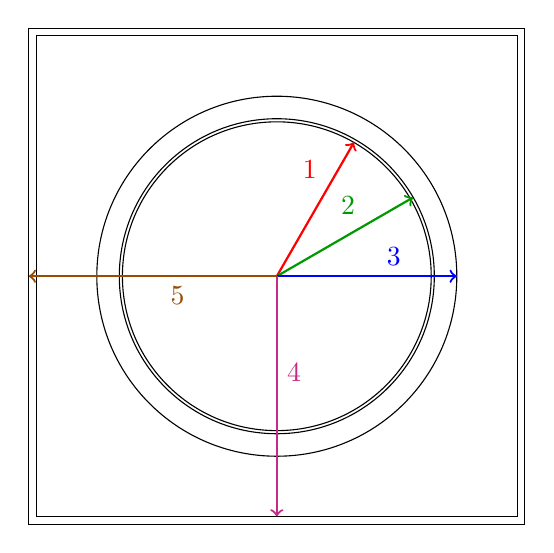
\begin{tikzpicture}[scale=5,auto]
        \draw (0,0) circle (0.39218);
      \draw[->,thick,red] (0,0) -- node[pos=0.65] {1} (0.196,0.34);
      \draw (0,0) circle (0.40005);
      \draw[->,thick,green!60!black] (0,0) -- node[pos=0.65] {2} (0.346,0.2);
      \draw (0,0) circle (0.4572);
      \draw[->,thick,blue] (0,0) -- node[pos=0.65] {3} (0.457,0.0);
      \draw (-0.61049,-0.61049) rectangle (0.61049,0.61049) ;
      \draw[->,thick,magenta!80!black] (0,0) -- node[pos=0.4] {4} (0.0,-0.61);
      \draw (-0.62992,-0.62992) rectangle (0.62992,0.62992) ;
      \draw[->,thick,orange!60!black] (0,0) -- node[pos=0.4] {5} (-0.63,0.0);

      \end{tikzpicture}
      \begin{tikzpicture}
       \matrix [matrix of nodes]
      {
          Arrow & Length (cm) & Material & \numrefheader\\
        \node[red]{1}; & \node[red]{0.39218}; & \node[red,hyperlink node=mat_fuel16]{Fuel}; & \node[red]{\ref{num:fuelpellrad}};\\ 
        \node[green!60!black]{2}; & \node[green!60!black]{0.40005}; & \node[green!60!black,hyperlink node=mat_helium]{Helium}; & \node[green!60!black]{\ref{num:fuelIRrad}};\\ 
        \node[blue]{3}; & \node[blue]{0.45720}; & \node[blue,hyperlink node=mat_zirc]{Zircaloy}; & \node[blue]{\ref{num:fuelORrad}};\\ 
        \node[magenta!80!black]{4}; & \node[magenta!80!black]{0.61049}; & \node[magenta!80!black,hyperlink node=mat_water]{Water}; & \node[magenta!80!black]{\ref{num:grid_spacer}};\\ 
        \node[orange!60!black]{5}; & \node[orange!60!black]{0.62992}; & \node[orange!60!black,hyperlink node=mat_inconel]{Zircaloy}; & \node[orange!60!black]{\ref{num:grid_spacer}};\\ 
      };
      \end{tikzpicture}

      \caption[Fuel pincell geometry for the intermediate grid spacer inner egg-crate]{ Fuel pincell geometry for the Zircaloy intermediate grid spacer inner egg-crate, chosen to have a thickness of 0.0194cm.  Source: \ref{num:grid_spacer} \label{fig_grid_pin_i}}
  \end{figure}

~

Figure \ref{fig_grid_assembly} shows the dimensions of the grid sleeve
assemblies in all grid spacer regions. To see what this looks like
in combination with the inner structural component in the pincells see Figure
\ref{fig_grid_assembly_zoom}, which shows an image of what the aggregate grid
spacer model looks like to scale.


\begin{figure}[htbp]
    \def\sleeveDim{10.74798}

    \centering
    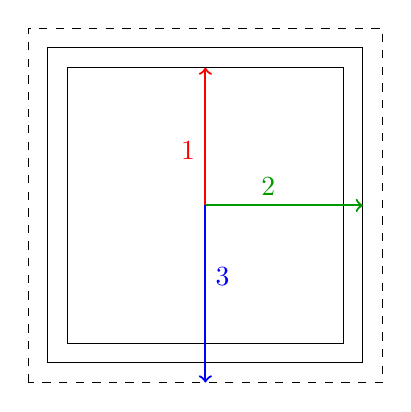
\begin{tikzpicture}[scale=5,auto]
      \draw (-0.35,-0.35) rectangle (0.35,0.35) ;
      \draw[->,thick,red] (0,0) -- node[pos=0.4] {1} (0.0,0.35);
      \draw (-0.4,-0.4) rectangle (0.4,0.4) ;
      \draw[->,thick,green!60!black] (0,0) -- node[pos=0.4] {2} (0.4,0.0);
      \draw[dashed] (-0.45,-0.45) rectangle (0.45,0.45);
      \draw[->,thick,blue] (0,0) -- node[pos=0.4] {3} (0,-0.45);
    \end{tikzpicture}
    \begin{tikzpicture}
     \matrix [matrix of nodes]
    {
        Arrow & Length (cm) & Material & \numrefheader \\
        \node[red]{1}; & \node[red]{10.70864}; & \node[red]{(Assembly)}; & \node[red]{\ref{num:grid_spacer}};\\
        \node[green!60!black]{2}; & \node[green!60!black]{\sleeveDim}; & \node[green!60!black]{(Grid Sleeve)}; & \node[green!60!black]{\ref{num:grid_spacer}};\\
        \node[blue]{3}; & \node[blue]{10.75182}; & \node[blue,hyperlink node=mat_water]{Water}; & \node[blue]{\ref{num:ass_pitch}};\\  
    };
    \end{tikzpicture}

    \caption[Schematic dimensions of stainless steel grid sleeve model]{Schematic
    dimensions of stainless steel grid sleeve. Arrow 1 is the half-width of 17
    times the pin lattice pitch; arrow 2 is the outer grid sleeve box
    half-width; arrow 3 is the outer boundary of the assembly pitch in the
    overall fuel assembly layout. The grid sleeve thickness was chosen as
    0.00384cm to conserve the estimated stainless steel mass. Source:
    \ref{num:grid_spacer}\label{fig_grid_assembly}}
\end{figure}

\begin{figure}[htbp]
    \centering
    \includegraphics[width=4in]{specifications/assy/figs/grid_zoom.png}

    \caption[Scale view of grid spacer model]{Scale view of an intermediate grid
    spacer showing inter-assembly spacing at a corner of position J14.
    Grey is Zircaloy, black is stainless steel, light blue is water, green is
    burnable absorber, white is air, and dark blue, red and yellow are the three
    different fuel enrichments.\label{fig_grid_assembly_zoom}}
\end{figure}

  \subsubsection{Core Specification}
\label{sec:corespec}

The remainder of the radial specification is made up of the building blocks 
defined in the previous sections. Specifically, the main core lattice of fuel
assemblies is made up of the previously described fuel assemblies, separated by
the fuel assembly lattice pitch specified in Table
\ref{table_assembly_overview}. In addition, specifications for the structural
components surrounding the fuel assembly lattice are given in Table
\ref{table_baff_vess}.


\begin{table}[htbp]
  \centering
  \caption{Structural component specifications. \label{table_baff_vess}}
  
  \begin{tabularx}{\textwidth}{l C c}
    \toprule
    & & Source \\
    \midrule
    \midrule 
    Baffle Width & 2.22250 cm & \ref{num:core_baffle}\\
    Baffle Water Gap & 0.1627 cm & \ref{num:rpv}\\
    Baffle Material & \hyperlink{mat_SS304}{Stainless Steel 304} & \ref{num:rpv}\\
    
    \\
    Core Barrel \ac{IR} & 187.960 cm & \ref{num:core_barrelIR}\\
    Core Barrel \ac{OR} & 193.675 cm & \ref{num:core_barrelOR}\\
    Core Barrel Material & \hyperlink{mat_SS304}{Stainless Steel 304} & \ref{num:core_barrelmat}\\
    \\
    Neutron Shield Panel \ac{IR} & 194.840 cm & \ref{num:rpv}\\
    Neutron Shield Panel \ac{OR} & 201.630 cm & \ref{num:rpv}\\
    Neutron Shield Panel Material & \hyperlink{mat_SS304}{Stainless Steel 304} & \ref{num:rpv}\\
    Neutron Shield Panel Width & $32^{\circ}$ at the $45^{\circ}$ marks & \ref{num:rpv}\\
    \\
    Pressure Vessel Liner \ac{IR} & 219.150 cm & \ref{num:rpv}\\
    Pressure Vessel Liner \ac{OR} & 219.710 cm & \ref{num:rpv}\\
    Pressure Vessel Liner Material & \hyperlink{mat_SS304}{Stainless Steel 304} & \ref{num:catawba}\\
    \\
    Pressure Vessel \ac{IR} & 219.710 cm & \ref{num:rpv}\\
    Pressure Vessel \ac{OR} & 241.300 cm & \ref{num:rpv}\\
    Pressure Vessel Material & \hyperlink{mat_carbonsteel}{Carbon Steel 508} & \ref{num:catawba}\\
    \bottomrule
  \end{tabularx}

\end{table}

%%%%%%%%%%%%%%%%%%%%%%%%%%%%%%%%%%%%%%%%%%%%%%%%%%%%%%%%%%%%%%%%%%%%%%%%%%%%%%%%
%\FloatBarrier
\paragraph{Enrichment Zones and Burnable Absorber Positions}
\label{sec:corespec_enrba}

The initial cycle 1 fuel assembly loading pattern is shown in Figure
\ref{fig_enr_ba_pos}, including the distribution of enrichments as well as
burnable absorber locations.  The burnable absorber configurations here are
described in Section \ref{sec:ba_configs}, rotated as appropriate for core
symmetry.  A scale view of burnable absorber pins depicting these rotations is
shown in Figure \ref{fig_ba_pos_real}.

\input{specifications/core/figs/cat_enr_ba_zones} % label: fig_enr_ba_pos

\begin{figure}[htbp]
    \centering
    \includegraphics[width=6in]{specifications/core/figs/cat_ba_positions.png}
    \caption[Cycle 1 detailed burnable absorber view]{Detailed scale view of
    burnable absorber pins in cycle 1, showing proper rotations.
    \label{fig_ba_pos_real}}
\end{figure}

Figure \ref{fig_enr_ba_pos_c2} shows the shuffling pattern for cycle 2, which
includes 64 fresh assemblies and a different burnable absorber pattern.


\begin{figure}[htbp]
    \centering
    
    % these dimensions are determined in arrow_dimms.ods

    \def\scale{1.0}

    \def\latWidth{0.2673473684*\scale}
    
    \def\RPVOR{3*\scale}
    \def\rectW{0.75*\scale}
    \def\RPVIR{2.7315789474*\scale}
    \def\BarrelIR{2.3368421053*\scale}
    \def\BarrelOR{2.4078947368*\scale}
    \def\ShieldIR{2.4223787816*\scale}
    \def\ShieldOR{2.5067965189*\scale}
    \def\LinerIR{2.7246166598*\scale}

    \def\bafCIRx{0.9357157895*\scale}
    \def\bafCIRy{2.0051052632*\scale}
    \def\bafCORx{0.9633473684*\scale}
    \def\bafCORy{2.0327368421*\scale}
    \def\bafMIRx{1.7377578947*\scale}
    \def\bafMIRy{1.4704105263*\scale}
    \def\bafMORx{1.7653894737*\scale}
    \def\bafMORy{1.4980421053*\scale}
    
    \tikzset{Assembly/.style={
        inner sep=0pt,
        text width=\latWidth in,
        minimum size=\latWidth in,
        draw=black,
        align=center
        }
    }
    
    \def\tkzRPV{(0,0) circle (\RPVIR) (0,0) circle (\RPVOR)}
    \def\tkzLiner{(0,0) circle (\LinerIR) (0,0) circle (\RPVIR)}
    \def\tkzBarrel{(0,0) circle (\BarrelIR) (0,0) circle (\BarrelOR)}
    \def\tkzShields{(0,0) circle (\ShieldIR) (0,0) circle (\ShieldOR)}
    
    \def\tkzBaffCOR{(-\bafCORx, -\bafCORy) rectangle (\bafCORx, \bafCORy)}
    \def\tkzBaffCIR{(-\bafCIRx, -\bafCIRy) rectangle (\bafCIRx, \bafCIRy)} 
    \def\tkzBaffMOR{(-\bafMORx, -\bafMORy) rectangle (\bafMORx, \bafMORy)}
    \def\tkzBaffMIR{(-\bafMIRx, -\bafMIRy) rectangle (\bafMIRx, \bafMIRy) }
    \def\tkzBaffleC{ \tkzBaffCIR \tkzBaffCOR }
    \def\tkzBaffleM{ \tkzBaffMIR \tkzBaffMOR }

    \def\tkzBaffCClip{\tkzBaffCIR (-\RPVOR, -\RPVOR) rectangle (\RPVOR, \RPVOR)}
    \def\tkzBaffMClip{\tkzBaffMIR (-\RPVOR, -\RPVOR) rectangle (\RPVOR, \RPVOR)}

    \def\noenr{black!10}
    \def\lowenr{green!60!black}
    \def\highenr{orange!90}

    \scalebox{1.0}{

      \begin{tikzpicture}[x=1in,y=1in]
      
        % draw RPV, barrel, and shield panels
        
        \path[fill=black!90!white,even odd rule] \tkzRPV;
        \path[fill=black,even odd rule] \tkzLiner;
        \path[fill=black,even odd rule] \tkzBarrel;
        \begin{scope}
          \clip (0,0) -- +(61:\RPVOR) arc (61:29:\RPVOR) --
                (0,0) -- +(151:\RPVOR) arc (151:119:\RPVOR) -- 
                (0,0) -- +(241:\RPVOR) arc (241:209:\RPVOR) -- 
                (0,0) -- +(331:\RPVOR) arc (331:299:\RPVOR) -- cycle;
          \path[fill=black,even odd rule] \tkzShields;
        \end{scope}

        % draw baffle north/south
        
        \begin{scope}[even odd rule]
          \clip[rotate=90] \tkzBaffMClip;
          \path[fill=black] \tkzBaffleC;
        \end{scope}
        \begin{scope}[even odd rule]
          \clip \tkzBaffCClip;
          \clip \tkzBaffMClip;
          \path[fill=black, rotate=90] \tkzBaffleM;
        \end{scope}
        
        % draw baffle east/west
        
        \begin{scope}[rotate=90]
          \begin{scope}[even odd rule]
            \clip[rotate=90] \tkzBaffMClip;
            \path[fill=black] \tkzBaffleC;
          \end{scope}
          \begin{scope}[even odd rule]
            \clip \tkzBaffCClip;
            \clip \tkzBaffMClip;
            \path[fill=black, rotate=90] \tkzBaffleM;
          \end{scope}
        \end{scope}
        
        % draw assembly row/column headers
        
        \draw[red, thick] ($(-7*\latWidth,\RPVOR/\latWidth*\latWidth)$) node[above, anchor=south] {R} -- ($(-7*\latWidth,4*\latWidth)$);
        \draw[red, thick] ($(-6*\latWidth,\RPVOR/\latWidth*\latWidth)$) node[above, anchor=south] {P} -- ($(-6*\latWidth,6*\latWidth)$);
        \draw[red, thick] ($(-5*\latWidth,\RPVOR/\latWidth*\latWidth)$) node[above, anchor=south] {N} -- ($(-5*\latWidth,7*\latWidth)$);
        \draw[red, thick] ($(-4*\latWidth,\RPVOR/\latWidth*\latWidth)$) node[above, anchor=south] {M} -- ($(-4*\latWidth,7*\latWidth)$);
        \draw[red, thick] ($(-3*\latWidth,\RPVOR/\latWidth*\latWidth)$) node[above, anchor=south] {L} -- ($(-3*\latWidth,8*\latWidth)$);
        \draw[red, thick] ($(-2*\latWidth,\RPVOR/\latWidth*\latWidth)$) node[above, anchor=south] {K} -- ($(-2*\latWidth,8*\latWidth)$);
        \draw[red, thick] ($(-1*\latWidth,\RPVOR/\latWidth*\latWidth)$) node[above, anchor=south] {J} -- ($(-1*\latWidth,8*\latWidth)$);
        \draw[red, thick] ($(-0*\latWidth,\RPVOR/\latWidth*\latWidth)$) node[above, anchor=south] {H} -- ($(-0*\latWidth,8*\latWidth)$);
        \draw[red, thick] ($(1*\latWidth,\RPVOR/\latWidth*\latWidth)$) node[above, anchor=south] {G} -- ($(1*\latWidth,8*\latWidth)$);
        \draw[red, thick] ($(2*\latWidth,\RPVOR/\latWidth*\latWidth)$) node[above, anchor=south] {F} -- ($(2*\latWidth,8*\latWidth)$);
        \draw[red, thick] ($(3*\latWidth,\RPVOR/\latWidth*\latWidth)$) node[above, anchor=south] {E} -- ($(3*\latWidth,8*\latWidth)$);
        \draw[red, thick] ($(4*\latWidth,\RPVOR/\latWidth*\latWidth)$) node[above, anchor=south] {D} -- ($(4*\latWidth,7*\latWidth)$);
        \draw[red, thick] ($(5*\latWidth,\RPVOR/\latWidth*\latWidth)$) node[above, anchor=south] {C} -- ($(5*\latWidth,7*\latWidth)$);
        \draw[red, thick] ($(6*\latWidth,\RPVOR/\latWidth*\latWidth)$) node[above, anchor=south] {B} -- ($(6*\latWidth,6*\latWidth)$);
        \draw[red, thick] ($(7*\latWidth,\RPVOR/\latWidth*\latWidth)$) node[above, anchor=south] {A} -- ($(7*\latWidth,4*\latWidth)$);
        
        \begin{scope}[rotate=90]
          \draw[red, thick] ($(-7*\latWidth,\RPVOR/\latWidth*\latWidth)$) node[left, anchor=east] {15} -- ($(-7*\latWidth,4*\latWidth)$);
          \draw[red, thick] ($(-6*\latWidth,\RPVOR/\latWidth*\latWidth)$) node[left, anchor=east] {14} -- ($(-6*\latWidth,6*\latWidth)$);
          \draw[red, thick] ($(-5*\latWidth,\RPVOR/\latWidth*\latWidth)$) node[left, anchor=east] {13} -- ($(-5*\latWidth,7*\latWidth)$);
          \draw[red, thick] ($(-4*\latWidth,\RPVOR/\latWidth*\latWidth)$) node[left, anchor=east] {12} -- ($(-4*\latWidth,7*\latWidth)$);
          \draw[red, thick] ($(-3*\latWidth,\RPVOR/\latWidth*\latWidth)$) node[left, anchor=east] {11} -- ($(-3*\latWidth,8*\latWidth)$);
          \draw[red, thick] ($(-2*\latWidth,\RPVOR/\latWidth*\latWidth)$) node[left, anchor=east] {10} -- ($(-2*\latWidth,8*\latWidth)$);
          \draw[red, thick] ($(-1*\latWidth,\RPVOR/\latWidth*\latWidth)$) node[left, anchor=east] {9} -- ($(-1*\latWidth,8*\latWidth)$);
          \draw[red, thick] ($(-0*\latWidth,\RPVOR/\latWidth*\latWidth)$) node[left, anchor=east] {8} -- ($(-0*\latWidth,8*\latWidth)$);
          \draw[red, thick] ($(1*\latWidth,\RPVOR/\latWidth*\latWidth)$) node[left, anchor=east] {7} -- ($(1*\latWidth,8*\latWidth)$);
          \draw[red, thick] ($(2*\latWidth,\RPVOR/\latWidth*\latWidth)$) node[left, anchor=east] {6} -- ($(2*\latWidth,8*\latWidth)$);
          \draw[red, thick] ($(3*\latWidth,\RPVOR/\latWidth*\latWidth)$) node[left, anchor=east] {5} -- ($(3*\latWidth,8*\latWidth)$);
          \draw[red, thick] ($(4*\latWidth,\RPVOR/\latWidth*\latWidth)$) node[left, anchor=east] {4} -- ($(4*\latWidth,7*\latWidth)$);
          \draw[red, thick] ($(5*\latWidth,\RPVOR/\latWidth*\latWidth)$) node[left, anchor=east] {3} -- ($(5*\latWidth,7*\latWidth)$);
          \draw[red, thick] ($(6*\latWidth,\RPVOR/\latWidth*\latWidth)$) node[left, anchor=east] {2} -- ($(6*\latWidth,6*\latWidth)$);
          \draw[red, thick] ($(7*\latWidth,\RPVOR/\latWidth*\latWidth)$) node[left, anchor=east] {1} -- ($(7*\latWidth,4*\latWidth)$);
        \end{scope}
        
        % draw fuel assembly nodes
        
        \node [Assembly, fill=\noenr] at ($(-3*\latWidth,7*\latWidth)$) {\scriptsize L10}; % L1
        \node [Assembly, fill=\highenr] at ($(-2*\latWidth,7*\latWidth)$) {}; % K1
        \node [Assembly, fill=\lowenr] at ($(-1*\latWidth,7*\latWidth)$) {}; % J1
        \node [Assembly, fill=\highenr] at ($(-0*\latWidth,7*\latWidth)$) {}; % H1
        \node [Assembly, fill=\lowenr] at ($( 1*\latWidth,7*\latWidth)$) {}; % G1
        \node [Assembly, fill=\highenr] at ($( 2*\latWidth,7*\latWidth)$) {}; % F1
        \node [Assembly, fill=\noenr] at ($( 3*\latWidth,7*\latWidth)$) {\scriptsize E10}; % E1

        \node [Assembly, fill=\noenr] at ($(-5*\latWidth,6*\latWidth)$) {\scriptsize G10}; % N2
        \node [Assembly, fill=\lowenr] at ($(-4*\latWidth,6*\latWidth)$) {}; % M2
        \node [Assembly, fill=\lowenr, hyperlink node=ass_4ba_target] at ($(-3*\latWidth,6*\latWidth)$) {\small 4}; % L2
        \node [Assembly, fill=\noenr] at ($(-2*\latWidth,6*\latWidth)$) {\scriptsize L02}; % K2
        \node [Assembly, fill=\noenr] at ($(-1*\latWidth,6*\latWidth)$) {\scriptsize P12}; % J2
        \node [Assembly, fill=\noenr] at ($(-0*\latWidth,6*\latWidth)$) {\scriptsize N03}; % H2
        \node [Assembly, fill=\noenr] at ($( 1*\latWidth,6*\latWidth)$) {\scriptsize B12}; % G2
        \node [Assembly, fill=\noenr] at ($( 2*\latWidth,6*\latWidth)$) {\scriptsize E02}; % F2
        \node [Assembly, fill=\lowenr, hyperlink node=ass_4ba_target] at ($( 3*\latWidth,6*\latWidth)$) {\small 4}; % E2
        \node [Assembly, fill=\lowenr] at ($( 4*\latWidth,6*\latWidth)$) {}; % D2
        \node [Assembly, fill=\noenr] at ($( 5*\latWidth,6*\latWidth)$) {\scriptsize J10}; % C2

        \node [Assembly, fill=\noenr] at ($(-6*\latWidth,5*\latWidth)$) {\scriptsize F09}; % P3
        \node [Assembly, fill=\highenr] at ($(-5*\latWidth,5*\latWidth)$) {}; % N3
        \node [Assembly, fill=\noenr] at ($(-4*\latWidth,5*\latWidth)$) {\scriptsize N02}; % M3
        \node [Assembly, fill=\noenr] at ($(-3*\latWidth,5*\latWidth)$) {\scriptsize N10}; % L3
        \node [Assembly, fill=\lowenr, hyperlink node=ass_8ba_target] at ($(-2*\latWidth,5*\latWidth)$) {\small 8}; % K3
        \node [Assembly, fill=\noenr] at ($(-1*\latWidth,5*\latWidth)$) {\scriptsize D11}; % J3
        \node [Assembly, fill=\noenr] at ($(-0*\latWidth,5*\latWidth)$) {\scriptsize R10}; % H3
        \node [Assembly, fill=\noenr] at ($( 1*\latWidth,5*\latWidth)$) {\scriptsize M11}; % G3
        \node [Assembly, fill=\lowenr, hyperlink node=ass_8ba_target] at ($( 2*\latWidth,5*\latWidth)$) {\small 8}; % F3
        \node [Assembly, fill=\noenr] at ($( 3*\latWidth,5*\latWidth)$) {\scriptsize C10}; % E3
        \node [Assembly, fill=\noenr] at ($( 4*\latWidth,5*\latWidth)$) {\scriptsize C02}; % D3
        \node [Assembly, fill=\highenr] at ($( 5*\latWidth,5*\latWidth)$) {}; % C3
        \node [Assembly, fill=\noenr] at ($( 6*\latWidth,5*\latWidth)$) {\scriptsize K09}; % B3

        \node [Assembly, fill=\lowenr] at ($(-6*\latWidth,4*\latWidth)$) {}; % P4
        \node [Assembly, fill=\noenr] at ($(-5*\latWidth,4*\latWidth)$) {\scriptsize P03}; % N4
        \node [Assembly, fill=\noenr] at ($(-4*\latWidth,4*\latWidth)$) {\scriptsize L08}; % M4
        \node [Assembly, fill=\lowenr, hyperlink node=ass_12ba_c2_target] at ($(-3*\latWidth,4*\latWidth)$) {\small 12}; % L4
        \node [Assembly, fill=\noenr] at ($(-2*\latWidth,4*\latWidth)$) {\scriptsize M09}; % K4
        \node [Assembly, fill=\noenr] at ($(-1*\latWidth,4*\latWidth)$) {\scriptsize E15}; % J4
        \node [Assembly, fill=\noenr] at ($(-0*\latWidth,4*\latWidth)$) {\scriptsize G08}; % H4
        \node [Assembly, fill=\noenr] at ($( 1*\latWidth,4*\latWidth)$) {\scriptsize L15}; % G4
        \node [Assembly, fill=\noenr] at ($( 2*\latWidth,4*\latWidth)$) {\scriptsize D09}; % F4
        \node [Assembly, fill=\lowenr, hyperlink node=ass_12ba_c2_target] at ($( 3*\latWidth,4*\latWidth)$) {\small 12}; % E4
        \node [Assembly, fill=\noenr] at ($( 4*\latWidth,4*\latWidth)$) {\scriptsize H05}; % D4
        \node [Assembly, fill=\noenr] at ($( 5*\latWidth,4*\latWidth)$) {\scriptsize B03}; % C4
        \node [Assembly, fill=\lowenr] at ($( 6*\latWidth,4*\latWidth)$) {}; % B4

        \node [Assembly, fill=\noenr] at ($(-7*\latWidth,3*\latWidth)$) {\scriptsize F05}; % R5
        \node [Assembly, fill=\lowenr, hyperlink node=ass_4ba_target] at ($(-6*\latWidth,3*\latWidth)$) {\small 4}; % P5
        \node [Assembly, fill=\noenr] at ($(-5*\latWidth,3*\latWidth)$) {\scriptsize F03}; % N5
        \node [Assembly, fill=\lowenr, hyperlink node=ass_12ba_c2_target] at ($(-4*\latWidth,3*\latWidth)$) {\small 12}; % M5
        \node [Assembly, fill=\noenr] at ($(-3*\latWidth,3*\latWidth)$) {\scriptsize M04}; % L5
        \node [Assembly, fill=\lowenr, hyperlink node=ass_8ba_target] at ($(-2*\latWidth,3*\latWidth)$) {\small 8}; % K5
        \node [Assembly, fill=\noenr] at ($(-1*\latWidth,3*\latWidth)$) {\scriptsize M03}; % J5
        \node [Assembly, fill=\noenr] at ($(-0*\latWidth,3*\latWidth)$) {\scriptsize A10}; % H5
        \node [Assembly, fill=\noenr] at ($( 1*\latWidth,3*\latWidth)$) {\scriptsize D03}; % G5
        \node [Assembly, fill=\lowenr, hyperlink node=ass_8ba_target] at ($( 2*\latWidth,3*\latWidth)$) {\small 8}; % F5
        \node [Assembly, fill=\noenr] at ($( 3*\latWidth,3*\latWidth)$) {\scriptsize D04}; % E5
        \node [Assembly, fill=\lowenr, hyperlink node=ass_12ba_c2_target] at ($( 4*\latWidth,3*\latWidth)$) {\small 12}; % D5
        \node [Assembly, fill=\noenr] at ($( 5*\latWidth,3*\latWidth)$) {\scriptsize K03}; % C5
        \node [Assembly, fill=\lowenr, hyperlink node=ass_4ba_target] at ($( 6*\latWidth,3*\latWidth)$) {\small 4}; % B5
        \node [Assembly, fill=\noenr] at ($( 7*\latWidth,3*\latWidth)$) {\scriptsize K05}; % A5

        \node [Assembly, fill=\highenr] at ($(-7*\latWidth,2*\latWidth)$) {}; % R6
        \node [Assembly, fill=\noenr] at ($(-6*\latWidth,2*\latWidth)$) {\scriptsize P05}; % P6
        \node [Assembly, fill=\lowenr, hyperlink node=ass_8ba_target] at ($(-5*\latWidth,2*\latWidth)$) {\small 8}; % N6
        \node [Assembly, fill=\noenr] at ($(-4*\latWidth,2*\latWidth)$) {\scriptsize G04}; % M6
        \node [Assembly, fill=\lowenr, hyperlink node=ass_8ba_target] at ($(-3*\latWidth,2*\latWidth)$) {\small 8}; % L6
        \node [Assembly, fill=\noenr] at ($(-2*\latWidth,2*\latWidth)$) {\scriptsize N08}; % K6
        \node [Assembly, fill=\noenr] at ($(-1*\latWidth,2*\latWidth)$) {\scriptsize R09}; % J6
        \node [Assembly, fill=\noenr] at ($(-0*\latWidth,2*\latWidth)$) {\scriptsize G14}; % H6
        \node [Assembly, fill=\noenr] at ($( 1*\latWidth,2*\latWidth)$) {\scriptsize A09}; % G6
        \node [Assembly, fill=\noenr] at ($( 2*\latWidth,2*\latWidth)$) {\scriptsize H03}; % F6
        \node [Assembly, fill=\lowenr, hyperlink node=ass_8ba_target] at ($( 3*\latWidth,2*\latWidth)$) {\small 8}; % E6
        \node [Assembly, fill=\noenr] at ($( 4*\latWidth,2*\latWidth)$) {\scriptsize J04}; % D6
        \node [Assembly, fill=\lowenr, hyperlink node=ass_8ba_target] at ($( 5*\latWidth,2*\latWidth)$) {\small 8}; % C6
        \node [Assembly, fill=\noenr] at ($( 6*\latWidth,2*\latWidth)$) {\scriptsize B05}; % B6
        \node [Assembly, fill=\highenr] at ($( 7*\latWidth,2*\latWidth)$) {}; % A6

        \node [Assembly, fill=\lowenr] at ($(-7*\latWidth,1*\latWidth)$) {}; % R7
        \node [Assembly, fill=\noenr] at ($(-6*\latWidth,1*\latWidth)$) {\scriptsize D02}; % P7
        \node [Assembly, fill=\noenr] at ($(-5*\latWidth,1*\latWidth)$) {\scriptsize E12}; % N7
        \node [Assembly, fill=\noenr] at ($(-4*\latWidth,1*\latWidth)$) {\scriptsize A11}; % M7
        \node [Assembly, fill=\noenr] at ($(-3*\latWidth,1*\latWidth)$) {\scriptsize N04}; % L7
        \node [Assembly, fill=\noenr] at ($(-2*\latWidth,1*\latWidth)$) {\scriptsize G01}; % K7
        \node [Assembly, fill=\noenr] at ($(-1*\latWidth,1*\latWidth)$) {\scriptsize B09}; % J7
        \node [Assembly, fill=\noenr] at ($(-0*\latWidth,1*\latWidth)$) {\scriptsize H15}; % H7
        \node [Assembly, fill=\noenr] at ($( 1*\latWidth,1*\latWidth)$) {\scriptsize J14}; % G7
        \node [Assembly, fill=\noenr] at ($( 2*\latWidth,1*\latWidth)$) {\scriptsize J01}; % F7
        \node [Assembly, fill=\noenr] at ($( 3*\latWidth,1*\latWidth)$) {\scriptsize C04}; % E7
        \node [Assembly, fill=\noenr] at ($( 4*\latWidth,1*\latWidth)$) {\scriptsize R11}; % D7
        \node [Assembly, fill=\noenr] at ($( 5*\latWidth,1*\latWidth)$) {\scriptsize L12}; % C7
        \node [Assembly, fill=\noenr] at ($( 6*\latWidth,1*\latWidth)$) {\scriptsize M02}; % B7
        \node [Assembly, fill=\lowenr] at ($( 7*\latWidth,1*\latWidth)$) {}; % A7

        \node [Assembly, fill=\highenr] at ($(-7*\latWidth,0*\latWidth)$) {}; % R8
        \node [Assembly, fill=\noenr] at ($(-6*\latWidth,0*\latWidth)$) {\scriptsize N13}; % P8
        \node [Assembly, fill=\noenr] at ($(-5*\latWidth,0*\latWidth)$) {\scriptsize F15}; % N8
        \node [Assembly, fill=\noenr] at ($(-4*\latWidth,0*\latWidth)$) {\scriptsize H07}; % M8
        \node [Assembly, fill=\noenr] at ($(-3*\latWidth,0*\latWidth)$) {\scriptsize F01}; % L8
        \node [Assembly, fill=\noenr] at ($(-2*\latWidth,0*\latWidth)$) {\scriptsize B07}; % K8
        \node [Assembly, fill=\noenr] at ($(-1*\latWidth,0*\latWidth)$) {\scriptsize A08}; % J8
        \node [Assembly, fill=\noenr] at ($(-0*\latWidth,0*\latWidth)$) {\scriptsize F14}; % H8
        \node [Assembly, fill=\noenr] at ($( 1*\latWidth,0*\latWidth)$) {\scriptsize R08}; % G8
        \node [Assembly, fill=\noenr] at ($( 2*\latWidth,0*\latWidth)$) {\scriptsize P09}; % F8
        \node [Assembly, fill=\noenr] at ($( 3*\latWidth,0*\latWidth)$) {\scriptsize K15}; % E8
        \node [Assembly, fill=\noenr] at ($( 4*\latWidth,0*\latWidth)$) {\scriptsize H09}; % D8
        \node [Assembly, fill=\noenr] at ($( 5*\latWidth,0*\latWidth)$) {\scriptsize K01}; % C8
        \node [Assembly, fill=\noenr] at ($( 6*\latWidth,0*\latWidth)$) {\scriptsize C03}; % B8
        \node [Assembly, fill=\highenr] at ($( 7*\latWidth,0*\latWidth)$) {}; % A8

        \node [Assembly, fill=\lowenr] at ($(-7*\latWidth,-1*\latWidth)$) {}; % R9
        \node [Assembly, fill=\noenr] at ($(-6*\latWidth,-1*\latWidth)$) {\scriptsize D14}; % P9
        \node [Assembly, fill=\noenr] at ($(-5*\latWidth,-1*\latWidth)$) {\scriptsize E04}; % N9
        \node [Assembly, fill=\noenr] at ($(-4*\latWidth,-1*\latWidth)$) {\scriptsize A05}; % M9
        \node [Assembly, fill=\noenr] at ($(-3*\latWidth,-1*\latWidth)$) {\scriptsize N12}; % L9
        \node [Assembly, fill=\noenr] at ($(-2*\latWidth,-1*\latWidth)$) {\scriptsize G15}; % K9
        \node [Assembly, fill=\noenr] at ($(-1*\latWidth,-1*\latWidth)$) {\scriptsize G02}; % J9
        \node [Assembly, fill=\noenr] at ($(-0*\latWidth,-1*\latWidth)$) {\scriptsize H01}; % H9
        \node [Assembly, fill=\noenr] at ($( 1*\latWidth,-1*\latWidth)$) {\scriptsize P07}; % G9
        \node [Assembly, fill=\noenr] at ($( 2*\latWidth,-1*\latWidth)$) {\scriptsize J15}; % F9
        \node [Assembly, fill=\noenr] at ($( 3*\latWidth,-1*\latWidth)$) {\scriptsize C12}; % E9
        \node [Assembly, fill=\noenr] at ($( 4*\latWidth,-1*\latWidth)$) {\scriptsize R05}; % D9
        \node [Assembly, fill=\noenr] at ($( 5*\latWidth,-1*\latWidth)$) {\scriptsize L04}; % C9
        \node [Assembly, fill=\noenr] at ($( 6*\latWidth,-1*\latWidth)$) {\scriptsize M14}; % B9
        \node [Assembly, fill=\lowenr] at ($( 7*\latWidth,-1*\latWidth)$) {}; % A9

        \node [Assembly, fill=\highenr] at ($(-7*\latWidth,-2*\latWidth)$) {}; % R10
        \node [Assembly, fill=\noenr] at ($(-6*\latWidth,-2*\latWidth)$) {\scriptsize P11}; % P10
        \node [Assembly, fill=\lowenr, hyperlink node=ass_8ba_target] at ($(-5*\latWidth,-2*\latWidth)$) {\small 8}; % N10
        \node [Assembly, fill=\noenr] at ($(-4*\latWidth,-2*\latWidth)$) {\scriptsize G12}; % M10
        \node [Assembly, fill=\lowenr, hyperlink node=ass_8ba_target] at ($(-3*\latWidth,-2*\latWidth)$) {\small 8}; % L10
        \node [Assembly, fill=\noenr] at ($(-2*\latWidth,-2*\latWidth)$) {\scriptsize H13}; % K10
        \node [Assembly, fill=\noenr] at ($(-1*\latWidth,-2*\latWidth)$) {\scriptsize R07}; % J10
        \node [Assembly, fill=\noenr] at ($(-0*\latWidth,-2*\latWidth)$) {\scriptsize J02}; % H10
        \node [Assembly, fill=\noenr] at ($( 1*\latWidth,-2*\latWidth)$) {\scriptsize A07}; % G10
        \node [Assembly, fill=\noenr] at ($( 2*\latWidth,-2*\latWidth)$) {\scriptsize C08}; % F10
        \node [Assembly, fill=\lowenr, hyperlink node=ass_8ba_target] at ($( 3*\latWidth,-2*\latWidth)$) {\small 8}; % E10
        \node [Assembly, fill=\noenr] at ($( 4*\latWidth,-2*\latWidth)$) {\scriptsize J12}; % D10
        \node [Assembly, fill=\lowenr, hyperlink node=ass_8ba_target] at ($( 5*\latWidth,-2*\latWidth)$) {\small 8}; % C10
        \node [Assembly, fill=\noenr] at ($( 6*\latWidth,-2*\latWidth)$) {\scriptsize B11}; % B10
        \node [Assembly, fill=\highenr] at ($( 7*\latWidth,-2*\latWidth)$) {}; % A10

        \node [Assembly, fill=\noenr] at ($(-7*\latWidth,-3*\latWidth)$) {\scriptsize F11}; % R11
        \node [Assembly, fill=\lowenr, hyperlink node=ass_4ba_target] at ($(-6*\latWidth,-3*\latWidth)$) {\small 4}; % P11
        \node [Assembly, fill=\noenr] at ($(-5*\latWidth,-3*\latWidth)$) {\scriptsize F13}; % N11
        \node [Assembly, fill=\lowenr, hyperlink node=ass_12ba_c2_target] at ($(-4*\latWidth,-3*\latWidth)$) {\small 12}; % M11
        \node [Assembly, fill=\noenr] at ($(-3*\latWidth,-3*\latWidth)$) {\scriptsize M12}; % L11
        \node [Assembly, fill=\lowenr, hyperlink node=ass_8ba_target] at ($(-2*\latWidth,-3*\latWidth)$) {\small 8}; % K11
        \node [Assembly, fill=\noenr] at ($(-1*\latWidth,-3*\latWidth)$) {\scriptsize M13}; % J11
        \node [Assembly, fill=\noenr] at ($(-0*\latWidth,-3*\latWidth)$) {\scriptsize R06}; % H11
        \node [Assembly, fill=\noenr] at ($( 1*\latWidth,-3*\latWidth)$) {\scriptsize D13}; % G11
        \node [Assembly, fill=\lowenr, hyperlink node=ass_8ba_target] at ($( 2*\latWidth,-3*\latWidth)$) {\small 8}; % F11
        \node [Assembly, fill=\noenr] at ($( 3*\latWidth,-3*\latWidth)$) {\scriptsize D12}; % E11
        \node [Assembly, fill=\lowenr, hyperlink node=ass_12ba_c2_target] at ($( 4*\latWidth,-3*\latWidth)$) {\small 12}; % D11
        \node [Assembly, fill=\noenr] at ($( 5*\latWidth,-3*\latWidth)$) {\scriptsize K13}; % C11
        \node [Assembly, fill=\lowenr, hyperlink node=ass_4ba_target] at ($( 6*\latWidth,-3*\latWidth)$) {\small 4}; % B11
        \node [Assembly, fill=\noenr] at ($( 7*\latWidth,-3*\latWidth)$) {\scriptsize K11}; % A11

        \node [Assembly, fill=\lowenr] at ($(-6*\latWidth,-4*\latWidth)$) {}; % P12
        \node [Assembly, fill=\noenr] at ($(-5*\latWidth,-4*\latWidth)$) {\scriptsize P13}; % N12
        \node [Assembly, fill=\noenr] at ($(-4*\latWidth,-4*\latWidth)$) {\scriptsize H11}; % M12
        \node [Assembly, fill=\lowenr, hyperlink node=ass_12ba_c2_target] at ($(-3*\latWidth,-4*\latWidth)$) {\small 12}; % L12
        \node [Assembly, fill=\noenr] at ($(-2*\latWidth,-4*\latWidth)$) {\scriptsize M07}; % K12
        \node [Assembly, fill=\noenr] at ($(-1*\latWidth,-4*\latWidth)$) {\scriptsize E01}; % J12
        \node [Assembly, fill=\noenr] at ($(-0*\latWidth,-4*\latWidth)$) {\scriptsize J08}; % H12
        \node [Assembly, fill=\noenr] at ($( 1*\latWidth,-4*\latWidth)$) {\scriptsize L01}; % G12
        \node [Assembly, fill=\noenr] at ($( 2*\latWidth,-4*\latWidth)$) {\scriptsize D07}; % F12
        \node [Assembly, fill=\lowenr, hyperlink node=ass_12ba_c2_target] at ($( 3*\latWidth,-4*\latWidth)$) {\small 12}; % E12
        \node [Assembly, fill=\noenr] at ($( 4*\latWidth,-4*\latWidth)$) {\scriptsize E08}; % D12
        \node [Assembly, fill=\noenr] at ($( 5*\latWidth,-4*\latWidth)$) {\scriptsize B13}; % C12
        \node [Assembly, fill=\lowenr] at ($( 6*\latWidth,-4*\latWidth)$) {}; % B12

        \node [Assembly, fill=\noenr] at ($(-6*\latWidth,-5*\latWidth)$) {\scriptsize F07}; % P13
        \node [Assembly, fill=\highenr] at ($(-5*\latWidth,-5*\latWidth)$) {}; % N13
        \node [Assembly, fill=\noenr] at ($(-4*\latWidth,-5*\latWidth)$) {\scriptsize N14}; % M13
        \node [Assembly, fill=\noenr] at ($(-3*\latWidth,-5*\latWidth)$) {\scriptsize N06}; % L13
        \node [Assembly, fill=\lowenr, hyperlink node=ass_8ba_target] at ($(-2*\latWidth,-5*\latWidth)$) {\small 8}; % K13
        \node [Assembly, fill=\noenr] at ($(-1*\latWidth,-5*\latWidth)$) {\scriptsize D05}; % J13
        \node [Assembly, fill=\noenr] at ($(-0*\latWidth,-5*\latWidth)$) {\scriptsize A06}; % H13
        \node [Assembly, fill=\noenr] at ($( 1*\latWidth,-5*\latWidth)$) {\scriptsize M05}; % G13
        \node [Assembly, fill=\lowenr, hyperlink node=ass_8ba_target] at ($( 2*\latWidth,-5*\latWidth)$) {\small 8}; % F13
        \node [Assembly, fill=\noenr] at ($( 3*\latWidth,-5*\latWidth)$) {\scriptsize C06}; % E13
        \node [Assembly, fill=\noenr] at ($( 4*\latWidth,-5*\latWidth)$) {\scriptsize C14}; % D13
        \node [Assembly, fill=\highenr] at ($( 5*\latWidth,-5*\latWidth)$) {}; % C13
        \node [Assembly, fill=\noenr] at ($( 6*\latWidth,-5*\latWidth)$) {\scriptsize K07}; % B13

        \node [Assembly, fill=\noenr] at ($(-5*\latWidth,-6*\latWidth)$) {\scriptsize G06}; % N14
        \node [Assembly, fill=\lowenr] at ($(-4*\latWidth,-6*\latWidth)$) {}; % M14
        \node [Assembly, fill=\lowenr, hyperlink node=ass_4ba_target] at ($(-3*\latWidth,-6*\latWidth)$) {\small 4}; % L14
        \node [Assembly, fill=\noenr] at ($(-2*\latWidth,-6*\latWidth)$) {\scriptsize L14}; % K14
        \node [Assembly, fill=\noenr] at ($(-1*\latWidth,-6*\latWidth)$) {\scriptsize P04}; % J14
        \node [Assembly, fill=\noenr] at ($(-0*\latWidth,-6*\latWidth)$) {\scriptsize C13}; % H14
        \node [Assembly, fill=\noenr] at ($( 1*\latWidth,-6*\latWidth)$) {\scriptsize B04}; % G14
        \node [Assembly, fill=\noenr] at ($( 2*\latWidth,-6*\latWidth)$) {\scriptsize E14}; % F14
        \node [Assembly, fill=\lowenr, hyperlink node=ass_4ba_target] at ($( 3*\latWidth,-6*\latWidth)$) {\small 4}; % E14
        \node [Assembly, fill=\lowenr] at ($( 4*\latWidth,-6*\latWidth)$) {}; % D14
        \node [Assembly, fill=\noenr] at ($( 5*\latWidth,-6*\latWidth)$) {\scriptsize J06}; % C14

        \node [Assembly, fill=\noenr] at ($(-3*\latWidth,-7*\latWidth)$) {\scriptsize L06}; % L15
        \node [Assembly, fill=\highenr] at ($(-2*\latWidth,-7*\latWidth)$) {}; % K15
        \node [Assembly, fill=\lowenr] at ($(-1*\latWidth,-7*\latWidth)$) {}; % J15
        \node [Assembly, fill=\highenr] at ($(-0*\latWidth,-7*\latWidth)$) {}; % H15
        \node [Assembly, fill=\lowenr] at ($( 1*\latWidth,-7*\latWidth)$) {}; % G15
        \node [Assembly, fill=\highenr] at ($( 2*\latWidth,-7*\latWidth)$) {}; % F15
        \node [Assembly, fill=\noenr] at ($( 3*\latWidth,-7*\latWidth)$) {\scriptsize E06}; % E15
        
      \end{tikzpicture}
    }
    
    % make the legend
    \begin{tikzpicture}
      \matrix [matrix of nodes]
          {
              \node [Assembly, fill=\lowenr, hyperlink node=mat_fuel32] at (0,0) {}; & \hyperref[mat_fuel32]{Fresh 3.2 w/o U235}~~~ & \node [Assembly, fill=\highenr, hyperlink node=mat_fuel34] at (0,0) {}; & \hyperref[mat_fuel34]{Fresh 3.4 w/o U235}~~~ \\
              \node [Assembly, fill=\noenr] at (0,0) {}; & Shuffled Assembly~~~ & ~~~ & ~~~\\
          };
    \end{tikzpicture}

    \caption[Cycle 2 shuffling pattern and burnable absorber positions]{Cycle 2 shuffling pattern, burnable absorber positions, and enrichment loading pattern of fresh assemblies. Sources: \ref{num:assycore}, \ref{num:c2shuffle} \label{fig_enr_ba_pos_c2}}
\end{figure}

 % label: fig_enr_ba_pos_c2

%%%%%%%%%%%%%%%%%%%%%%%%%%%%%%%%%%%%%%%%%%%%%%%%%%%%%%%%%%%%%%%%%%%%%%%%%%%%%%%%
%\FloatBarrier
\paragraph{Control Rod Bank Positions}

Each of the four control rod banks - specified by the identifiers A, B, C, and D
- are made up of several control rod clusters in multiple fuel assemblies. In
control rod clusters, every guide tube is filled with the control rod pincell
described in section \ref{sec:pintypes}, with the exception of the center
tube. Each of the clusters in a given control rod bank move together.

In addition to the control rod banks, 5 shutdown banks of control rod clusters
are included above the core - specified by $\mathrm{S}_\mathrm{A}$,
$\mathrm{S}_\mathrm{B}$, $\mathrm{S}_\mathrm{C}$, $\mathrm{S}_\mathrm{D}$, and
$\mathrm{S}_\mathrm{E}$. These clusters are not used in normal operation,
however, their reactivity worth was measured and reported in Table
\ref{tbl:meas_c1phys}.

Figure \ref{fig_cr_pos} shows the radial locations of control rod clusters
belonging to each control rod and shutdown bank. The axial specifications of
each are described later in Section \ref{sec:axial_cr}.

The positions of control rod banks do not change between cycle 1 and cycle 2.


\begin{figure}[htbp]
    \centering
    
    % these dimensions are determined in arrow_dimms.ods

    \def\scale{1.0}

    \def\latWidth{0.2673473684*\scale}
    
    \def\RPVOR{3*\scale}
    \def\rectW{0.75*\scale}
    \def\RPVIR{2.7315789474*\scale}
    \def\BarrelIR{2.3368421053*\scale}
    \def\BarrelOR{2.4078947368*\scale}
    \def\ShieldIR{2.4223787816*\scale}
    \def\ShieldOR{2.5067965189*\scale}
    \def\LinerIR{2.7246166598*\scale}

    \def\bafCIRx{0.9357157895*\scale}
    \def\bafCIRy{2.0051052632*\scale}
    \def\bafCORx{0.9633473684*\scale}
    \def\bafCORy{2.0327368421*\scale}
    \def\bafMIRx{1.7377578947*\scale}
    \def\bafMIRy{1.4704105263*\scale}
    \def\bafMORx{1.7653894737*\scale}
    \def\bafMORy{1.4980421053*\scale}
    
    \tikzset{Assembly/.style={
        inner sep=0pt,
        text width=\latWidth in,
        minimum size=\latWidth in,
        draw=black,
        align=center
        }
    }
    
    \def\tkzRPV{(0,0) circle (\RPVIR) (0,0) circle (\RPVOR)}
    \def\tkzLiner{(0,0) circle (\LinerIR) (0,0) circle (\RPVIR)}
    \def\tkzBarrel{(0,0) circle (\BarrelIR) (0,0) circle (\BarrelOR)}
    \def\tkzShields{(0,0) circle (\ShieldIR) (0,0) circle (\ShieldOR)}
    
    \def\tkzBaffCOR{(-\bafCORx, -\bafCORy) rectangle (\bafCORx, \bafCORy)}
    \def\tkzBaffCIR{(-\bafCIRx, -\bafCIRy) rectangle (\bafCIRx, \bafCIRy)} 
    \def\tkzBaffMOR{(-\bafMORx, -\bafMORy) rectangle (\bafMORx, \bafMORy)}
    \def\tkzBaffMIR{(-\bafMIRx, -\bafMIRy) rectangle (\bafMIRx, \bafMIRy) }
    \def\tkzBaffleC{ \tkzBaffCIR \tkzBaffCOR }
    \def\tkzBaffleM{ \tkzBaffMIR \tkzBaffMOR }

    \def\tkzBaffCClip{\tkzBaffCIR (-\RPVOR, -\RPVOR) rectangle (\RPVOR, \RPVOR)}
    \def\tkzBaffMClip{\tkzBaffMIR (-\RPVOR, -\RPVOR) rectangle (\RPVOR, \RPVOR)}

    \def\highenr{blue!50}
    \def\midenr{yellow!50}
    \def\lowenr{red!50}

    \scalebox{1.0}{

      \begin{tikzpicture}[x=1in,y=1in]
      
        % draw RPV, barrel, liner and shield panels
        
        \path[fill=black!90!white,even odd rule] \tkzRPV;
        \path[fill=black,even odd rule] \tkzLiner;
        \path[fill=black,even odd rule] \tkzBarrel;
        \begin{scope}
          \clip (0,0) -- +(61:\RPVOR) arc (61:29:\RPVOR) --
                (0,0) -- +(151:\RPVOR) arc (151:119:\RPVOR) -- 
                (0,0) -- +(241:\RPVOR) arc (241:209:\RPVOR) -- 
                (0,0) -- +(331:\RPVOR) arc (331:299:\RPVOR) -- cycle;
          \path[fill=black,even odd rule] \tkzShields;
        \end{scope}

        % draw baffle north/south
        
        \begin{scope}[even odd rule]
          \clip[rotate=90] \tkzBaffMClip;
          \path[fill=black] \tkzBaffleC;
        \end{scope}
        \begin{scope}[even odd rule]
          \clip \tkzBaffCClip;
          \clip \tkzBaffMClip;
          \path[fill=black, rotate=90] \tkzBaffleM;
        \end{scope}
        
        % draw baffle east/west
        
        \begin{scope}[rotate=90]
          \begin{scope}[even odd rule]
            \clip[rotate=90] \tkzBaffMClip;
            \path[fill=black] \tkzBaffleC;
          \end{scope}
          \begin{scope}[even odd rule]
            \clip \tkzBaffCClip;
            \clip \tkzBaffMClip;
            \path[fill=black, rotate=90] \tkzBaffleM;
          \end{scope}
        \end{scope}
        
        % draw assembly row/column headers
        
        \draw[red, thick] ($(-7*\latWidth,\RPVOR/\latWidth*\latWidth)$) node[above, anchor=south] {R} -- ($(-7*\latWidth,4*\latWidth)$);
        \draw[red, thick] ($(-6*\latWidth,\RPVOR/\latWidth*\latWidth)$) node[above, anchor=south] {P} -- ($(-6*\latWidth,6*\latWidth)$);
        \draw[red, thick] ($(-5*\latWidth,\RPVOR/\latWidth*\latWidth)$) node[above, anchor=south] {N} -- ($(-5*\latWidth,7*\latWidth)$);
        \draw[red, thick] ($(-4*\latWidth,\RPVOR/\latWidth*\latWidth)$) node[above, anchor=south] {M} -- ($(-4*\latWidth,7*\latWidth)$);
        \draw[red, thick] ($(-3*\latWidth,\RPVOR/\latWidth*\latWidth)$) node[above, anchor=south] {L} -- ($(-3*\latWidth,8*\latWidth)$);
        \draw[red, thick] ($(-2*\latWidth,\RPVOR/\latWidth*\latWidth)$) node[above, anchor=south] {K} -- ($(-2*\latWidth,8*\latWidth)$);
        \draw[red, thick] ($(-1*\latWidth,\RPVOR/\latWidth*\latWidth)$) node[above, anchor=south] {J} -- ($(-1*\latWidth,8*\latWidth)$);
        \draw[red, thick] ($(-0*\latWidth,\RPVOR/\latWidth*\latWidth)$) node[above, anchor=south] {H} -- ($(-0*\latWidth,8*\latWidth)$);
        \draw[red, thick] ($(1*\latWidth,\RPVOR/\latWidth*\latWidth)$) node[above, anchor=south] {G} -- ($(1*\latWidth,8*\latWidth)$);
        \draw[red, thick] ($(2*\latWidth,\RPVOR/\latWidth*\latWidth)$) node[above, anchor=south] {F} -- ($(2*\latWidth,8*\latWidth)$);
        \draw[red, thick] ($(3*\latWidth,\RPVOR/\latWidth*\latWidth)$) node[above, anchor=south] {E} -- ($(3*\latWidth,8*\latWidth)$);
        \draw[red, thick] ($(4*\latWidth,\RPVOR/\latWidth*\latWidth)$) node[above, anchor=south] {D} -- ($(4*\latWidth,7*\latWidth)$);
        \draw[red, thick] ($(5*\latWidth,\RPVOR/\latWidth*\latWidth)$) node[above, anchor=south] {C} -- ($(5*\latWidth,7*\latWidth)$);
        \draw[red, thick] ($(6*\latWidth,\RPVOR/\latWidth*\latWidth)$) node[above, anchor=south] {B} -- ($(6*\latWidth,6*\latWidth)$);
        \draw[red, thick] ($(7*\latWidth,\RPVOR/\latWidth*\latWidth)$) node[above, anchor=south] {A} -- ($(7*\latWidth,4*\latWidth)$);
        
        \begin{scope}[rotate=90]
          \draw[red, thick] ($(-7*\latWidth,\RPVOR/\latWidth*\latWidth)$) node[left, anchor=east] {15} -- ($(-7*\latWidth,4*\latWidth)$);
          \draw[red, thick] ($(-6*\latWidth,\RPVOR/\latWidth*\latWidth)$) node[left, anchor=east] {14} -- ($(-6*\latWidth,6*\latWidth)$);
          \draw[red, thick] ($(-5*\latWidth,\RPVOR/\latWidth*\latWidth)$) node[left, anchor=east] {13} -- ($(-5*\latWidth,7*\latWidth)$);
          \draw[red, thick] ($(-4*\latWidth,\RPVOR/\latWidth*\latWidth)$) node[left, anchor=east] {12} -- ($(-4*\latWidth,7*\latWidth)$);
          \draw[red, thick] ($(-3*\latWidth,\RPVOR/\latWidth*\latWidth)$) node[left, anchor=east] {11} -- ($(-3*\latWidth,8*\latWidth)$);
          \draw[red, thick] ($(-2*\latWidth,\RPVOR/\latWidth*\latWidth)$) node[left, anchor=east] {10} -- ($(-2*\latWidth,8*\latWidth)$);
          \draw[red, thick] ($(-1*\latWidth,\RPVOR/\latWidth*\latWidth)$) node[left, anchor=east] {9} -- ($(-1*\latWidth,8*\latWidth)$);
          \draw[red, thick] ($(-0*\latWidth,\RPVOR/\latWidth*\latWidth)$) node[left, anchor=east] {8} -- ($(-0*\latWidth,8*\latWidth)$);
          \draw[red, thick] ($(1*\latWidth,\RPVOR/\latWidth*\latWidth)$) node[left, anchor=east] {7} -- ($(1*\latWidth,8*\latWidth)$);
          \draw[red, thick] ($(2*\latWidth,\RPVOR/\latWidth*\latWidth)$) node[left, anchor=east] {6} -- ($(2*\latWidth,8*\latWidth)$);
          \draw[red, thick] ($(3*\latWidth,\RPVOR/\latWidth*\latWidth)$) node[left, anchor=east] {5} -- ($(3*\latWidth,8*\latWidth)$);
          \draw[red, thick] ($(4*\latWidth,\RPVOR/\latWidth*\latWidth)$) node[left, anchor=east] {4} -- ($(4*\latWidth,7*\latWidth)$);
          \draw[red, thick] ($(5*\latWidth,\RPVOR/\latWidth*\latWidth)$) node[left, anchor=east] {3} -- ($(5*\latWidth,7*\latWidth)$);
          \draw[red, thick] ($(6*\latWidth,\RPVOR/\latWidth*\latWidth)$) node[left, anchor=east] {2} -- ($(6*\latWidth,6*\latWidth)$);
          \draw[red, thick] ($(7*\latWidth,\RPVOR/\latWidth*\latWidth)$) node[left, anchor=east] {1} -- ($(7*\latWidth,4*\latWidth)$);
        \end{scope}
        
        % draw fuel assembly nodes
        
        \node [Assembly, fill=\highenr] at ($(-3*\latWidth,7*\latWidth)$) {}; % L1
        \node [Assembly, fill=\highenr] at ($(-2*\latWidth,7*\latWidth)$) {}; % K1
        \node [Assembly, fill=\highenr] at ($(-1*\latWidth,7*\latWidth)$) {}; % J1
        \node [Assembly, fill=\highenr] at ($(-0*\latWidth,7*\latWidth)$) {}; % H1
        \node [Assembly, fill=\highenr] at ($( 1*\latWidth,7*\latWidth)$) {}; % G1
        \node [Assembly, fill=\highenr] at ($( 2*\latWidth,7*\latWidth)$) {}; % F1
        \node [Assembly, fill=\highenr] at ($( 3*\latWidth,7*\latWidth)$) {}; % E1

        \node [Assembly, fill=\highenr] at ($(-5*\latWidth,6*\latWidth)$) {}; % N2
        \node [Assembly, fill=\highenr] at ($(-4*\latWidth,6*\latWidth)$) {$\mathrm{S}_\mathrm{A}$}; % M2
        \node [Assembly, fill=\highenr] at ($(-3*\latWidth,6*\latWidth)$) {}; % L2
        \node [Assembly, fill=\lowenr] at ($(-2*\latWidth,6*\latWidth)$) {$\mathrm{B}$}; % K2
        \node [Assembly, fill=\highenr] at ($(-1*\latWidth,6*\latWidth)$) {}; % J2
        \node [Assembly, fill=\lowenr] at ($(-0*\latWidth,6*\latWidth)$) {$\mathrm{C}$}; % H2
        \node [Assembly, fill=\highenr] at ($( 1*\latWidth,6*\latWidth)$) {}; % G2
        \node [Assembly, fill=\lowenr] at ($( 2*\latWidth,6*\latWidth)$) {$\mathrm{B}$}; % F2
        \node [Assembly, fill=\highenr] at ($( 3*\latWidth,6*\latWidth)$) {}; % E2
        \node [Assembly, fill=\highenr] at ($( 4*\latWidth,6*\latWidth)$) {$\mathrm{S}_\mathrm{A}$}; % D2
        \node [Assembly, fill=\highenr] at ($( 5*\latWidth,6*\latWidth)$) {}; % C2

        \node [Assembly, fill=\highenr] at ($(-6*\latWidth,5*\latWidth)$) {}; % P3
        \node [Assembly, fill=\highenr] at ($(-5*\latWidth,5*\latWidth)$) {}; % N3
        \node [Assembly, fill=\midenr] at ($(-4*\latWidth,5*\latWidth)$) {}; % M3
        \node [Assembly, fill=\lowenr] at ($(-3*\latWidth,5*\latWidth)$) {$\mathrm{S}_\mathrm{D}$}; % L3
        \node [Assembly, fill=\midenr] at ($(-2*\latWidth,5*\latWidth)$) {}; % K3
        \node [Assembly, fill=\lowenr] at ($(-1*\latWidth,5*\latWidth)$) {$\mathrm{S}_\mathrm{B}$}; % J3
        \node [Assembly, fill=\midenr] at ($(-0*\latWidth,5*\latWidth)$) {}; % H3
        \node [Assembly, fill=\lowenr] at ($( 1*\latWidth,5*\latWidth)$) {$\mathrm{S}_\mathrm{B}$}; % G3
        \node [Assembly, fill=\midenr] at ($( 2*\latWidth,5*\latWidth)$) {}; % F3
        \node [Assembly, fill=\lowenr] at ($( 3*\latWidth,5*\latWidth)$) {$\mathrm{S}_\mathrm{C}$}; % E3
        \node [Assembly, fill=\midenr] at ($( 4*\latWidth,5*\latWidth)$) {}; % D3
        \node [Assembly, fill=\highenr] at ($( 5*\latWidth,5*\latWidth)$) {}; % C3
        \node [Assembly, fill=\highenr] at ($( 6*\latWidth,5*\latWidth)$) {}; % B3

        \node [Assembly, fill=\highenr] at ($(-6*\latWidth,4*\latWidth)$) {$\mathrm{S}_\mathrm{A}$}; % P4
        \node [Assembly, fill=\midenr] at ($(-5*\latWidth,4*\latWidth)$) {}; % N4
        \node [Assembly, fill=\midenr] at ($(-4*\latWidth,4*\latWidth)$) {$\mathrm{D}$}; % M4
        \node [Assembly, fill=\midenr] at ($(-3*\latWidth,4*\latWidth)$) {}; % L4
        \node [Assembly, fill=\lowenr] at ($(-2*\latWidth,4*\latWidth)$) {}; % K4
        \node [Assembly, fill=\midenr] at ($(-1*\latWidth,4*\latWidth)$) {}; % J4
        \node [Assembly, fill=\lowenr] at ($(-0*\latWidth,4*\latWidth)$) {$\mathrm{S}_\mathrm{E}$}; % H4
        \node [Assembly, fill=\midenr] at ($( 1*\latWidth,4*\latWidth)$) {}; % G4
        \node [Assembly, fill=\lowenr] at ($( 2*\latWidth,4*\latWidth)$) {}; % F4
        \node [Assembly, fill=\midenr] at ($( 3*\latWidth,4*\latWidth)$) {}; % E4
        \node [Assembly, fill=\midenr] at ($( 4*\latWidth,4*\latWidth)$) {$\mathrm{D}$}; % D4
        \node [Assembly, fill=\midenr] at ($( 5*\latWidth,4*\latWidth)$) {}; % C4
        \node [Assembly, fill=\highenr] at ($( 6*\latWidth,4*\latWidth)$) {$\mathrm{S}_\mathrm{A}$}; % B4

        \node [Assembly, fill=\highenr] at ($(-7*\latWidth,3*\latWidth)$) {}; % R5
        \node [Assembly, fill=\highenr] at ($(-6*\latWidth,3*\latWidth)$) {}; % P5
        \node [Assembly, fill=\lowenr] at ($(-5*\latWidth,3*\latWidth)$) {$\mathrm{S}_\mathrm{C}$}; % N5
        \node [Assembly, fill=\midenr] at ($(-4*\latWidth,3*\latWidth)$) {}; % M5
        \node [Assembly, fill=\lowenr] at ($(-3*\latWidth,3*\latWidth)$) {}; % L5
        \node [Assembly, fill=\midenr] at ($(-2*\latWidth,3*\latWidth)$) {}; % K5
        \node [Assembly, fill=\lowenr] at ($(-1*\latWidth,3*\latWidth)$) {}; % J5
        \node [Assembly, fill=\midenr] at ($(-0*\latWidth,3*\latWidth)$) {}; % H5
        \node [Assembly, fill=\lowenr] at ($( 1*\latWidth,3*\latWidth)$) {}; % G5
        \node [Assembly, fill=\midenr] at ($( 2*\latWidth,3*\latWidth)$) {}; % F5
        \node [Assembly, fill=\lowenr] at ($( 3*\latWidth,3*\latWidth)$) {}; % E5
        \node [Assembly, fill=\midenr] at ($( 4*\latWidth,3*\latWidth)$) {}; % D5
        \node [Assembly, fill=\lowenr] at ($( 5*\latWidth,3*\latWidth)$) {$\mathrm{S}_\mathrm{D}$}; % C5
        \node [Assembly, fill=\highenr] at ($( 6*\latWidth,3*\latWidth)$) {}; % B5
        \node [Assembly, fill=\highenr] at ($( 7*\latWidth,3*\latWidth)$) {}; % A5

        \node [Assembly, fill=\highenr] at ($(-7*\latWidth,2*\latWidth)$) {}; % R6
        \node [Assembly, fill=\lowenr] at ($(-6*\latWidth,2*\latWidth)$) {$\mathrm{B}$}; % P6
        \node [Assembly, fill=\midenr] at ($(-5*\latWidth,2*\latWidth)$) {}; % N6
        \node [Assembly, fill=\lowenr] at ($(-4*\latWidth,2*\latWidth)$) {}; % M6
        \node [Assembly, fill=\midenr] at ($(-3*\latWidth,2*\latWidth)$) {}; % L6
        \node [Assembly, fill=\lowenr] at ($(-2*\latWidth,2*\latWidth)$) {$\mathrm{C}$}; % K6
        \node [Assembly, fill=\midenr] at ($(-1*\latWidth,2*\latWidth)$) {}; % J6
        \node [Assembly, fill=\lowenr] at ($(-0*\latWidth,2*\latWidth)$) {$\mathrm{A}$}; % H6
        \node [Assembly, fill=\midenr] at ($( 1*\latWidth,2*\latWidth)$) {}; % G6
        \node [Assembly, fill=\lowenr] at ($( 2*\latWidth,2*\latWidth)$) {$\mathrm{C}$}; % F6
        \node [Assembly, fill=\midenr] at ($( 3*\latWidth,2*\latWidth)$) {}; % E6
        \node [Assembly, fill=\lowenr] at ($( 4*\latWidth,2*\latWidth)$) {}; % D6
        \node [Assembly, fill=\midenr] at ($( 5*\latWidth,2*\latWidth)$) {}; % C6
        \node [Assembly, fill=\lowenr] at ($( 6*\latWidth,2*\latWidth)$) {$\mathrm{B}$}; % B6
        \node [Assembly, fill=\highenr] at ($( 7*\latWidth,2*\latWidth)$) {}; % A6

        \node [Assembly, fill=\highenr] at ($(-7*\latWidth,1*\latWidth)$) {}; % R7
        \node [Assembly, fill=\highenr] at ($(-6*\latWidth,1*\latWidth)$) {}; % P7
        \node [Assembly, fill=\lowenr] at ($(-5*\latWidth,1*\latWidth)$) {$\mathrm{S}_\mathrm{B}$}; % N7
        \node [Assembly, fill=\midenr] at ($(-4*\latWidth,1*\latWidth)$) {}; % M7
        \node [Assembly, fill=\lowenr] at ($(-3*\latWidth,1*\latWidth)$) {}; % L7
        \node [Assembly, fill=\midenr] at ($(-2*\latWidth,1*\latWidth)$) {}; % K7
        \node [Assembly, fill=\lowenr] at ($(-1*\latWidth,1*\latWidth)$) {}; % J7
        \node [Assembly, fill=\midenr] at ($(-0*\latWidth,1*\latWidth)$) {}; % H7
        \node [Assembly, fill=\lowenr] at ($( 1*\latWidth,1*\latWidth)$) {}; % G7
        \node [Assembly, fill=\midenr] at ($( 2*\latWidth,1*\latWidth)$) {}; % F7
        \node [Assembly, fill=\lowenr] at ($( 3*\latWidth,1*\latWidth)$) {}; % E7
        \node [Assembly, fill=\midenr] at ($( 4*\latWidth,1*\latWidth)$) {}; % D7
        \node [Assembly, fill=\lowenr] at ($( 5*\latWidth,1*\latWidth)$) {$\mathrm{S}_\mathrm{B}$}; % C7
        \node [Assembly, fill=\highenr] at ($( 6*\latWidth,1*\latWidth)$) {}; % B7
        \node [Assembly, fill=\highenr] at ($( 7*\latWidth,1*\latWidth)$) {}; % A7

        \node [Assembly, fill=\highenr] at ($(-7*\latWidth,0*\latWidth)$) {}; % R8
        \node [Assembly, fill=\lowenr] at ($(-6*\latWidth,0*\latWidth)$) {$\mathrm{C}$}; % P8
        \node [Assembly, fill=\midenr] at ($(-5*\latWidth,0*\latWidth)$) {}; % N8
        \node [Assembly, fill=\lowenr] at ($(-4*\latWidth,0*\latWidth)$) {$\mathrm{S}_\mathrm{E}$}; % M8
        \node [Assembly, fill=\midenr] at ($(-3*\latWidth,0*\latWidth)$) {}; % L8
        \node [Assembly, fill=\lowenr] at ($(-2*\latWidth,0*\latWidth)$) {$\mathrm{A}$}; % K8
        \node [Assembly, fill=\midenr] at ($(-1*\latWidth,0*\latWidth)$) {}; % J8
        \node [Assembly, fill=\lowenr] at ($(-0*\latWidth,0*\latWidth)$) {$\mathrm{D}$}; % H8
        \node [Assembly, fill=\midenr] at ($( 1*\latWidth,0*\latWidth)$) {}; % G8
        \node [Assembly, fill=\lowenr] at ($( 2*\latWidth,0*\latWidth)$) {$\mathrm{A}$}; % F8
        \node [Assembly, fill=\midenr] at ($( 3*\latWidth,0*\latWidth)$) {}; % E8
        \node [Assembly, fill=\lowenr] at ($( 4*\latWidth,0*\latWidth)$) {$\mathrm{S}_\mathrm{E}$}; % D8
        \node [Assembly, fill=\midenr] at ($( 5*\latWidth,0*\latWidth)$) {}; % C8
        \node [Assembly, fill=\lowenr] at ($( 6*\latWidth,0*\latWidth)$) {$\mathrm{C}$}; % B8
        \node [Assembly, fill=\highenr] at ($( 7*\latWidth,0*\latWidth)$) {}; % A8

        \node [Assembly, fill=\highenr] at ($(-7*\latWidth,-1*\latWidth)$) {}; % R9
        \node [Assembly, fill=\highenr] at ($(-6*\latWidth,-1*\latWidth)$) {}; % P9
        \node [Assembly, fill=\lowenr] at ($(-5*\latWidth,-1*\latWidth)$) {$\mathrm{S}_\mathrm{B}$}; % N9
        \node [Assembly, fill=\midenr] at ($(-4*\latWidth,-1*\latWidth)$) {}; % M9
        \node [Assembly, fill=\lowenr] at ($(-3*\latWidth,-1*\latWidth)$) {}; % L9
        \node [Assembly, fill=\midenr] at ($(-2*\latWidth,-1*\latWidth)$) {}; % K9
        \node [Assembly, fill=\lowenr] at ($(-1*\latWidth,-1*\latWidth)$) {}; % J9
        \node [Assembly, fill=\midenr] at ($(-0*\latWidth,-1*\latWidth)$) {}; % H9
        \node [Assembly, fill=\lowenr] at ($( 1*\latWidth,-1*\latWidth)$) {}; % G9
        \node [Assembly, fill=\midenr] at ($( 2*\latWidth,-1*\latWidth)$) {}; % F9
        \node [Assembly, fill=\lowenr] at ($( 3*\latWidth,-1*\latWidth)$) {}; % E9
        \node [Assembly, fill=\midenr] at ($( 4*\latWidth,-1*\latWidth)$) {}; % D9
        \node [Assembly, fill=\lowenr] at ($( 5*\latWidth,-1*\latWidth)$) {$\mathrm{S}_\mathrm{B}$}; % C9
        \node [Assembly, fill=\highenr] at ($( 6*\latWidth,-1*\latWidth)$) {}; % B9
        \node [Assembly, fill=\highenr] at ($( 7*\latWidth,-1*\latWidth)$) {}; % A9

        \node [Assembly, fill=\highenr] at ($(-7*\latWidth,-2*\latWidth)$) {}; % R10
        \node [Assembly, fill=\lowenr] at ($(-6*\latWidth,-2*\latWidth)$) {$\mathrm{B}$}; % P10
        \node [Assembly, fill=\midenr] at ($(-5*\latWidth,-2*\latWidth)$) {}; % N10
        \node [Assembly, fill=\lowenr] at ($(-4*\latWidth,-2*\latWidth)$) {}; % M10
        \node [Assembly, fill=\midenr] at ($(-3*\latWidth,-2*\latWidth)$) {}; % L10
        \node [Assembly, fill=\lowenr] at ($(-2*\latWidth,-2*\latWidth)$) {$\mathrm{C}$}; % K10
        \node [Assembly, fill=\midenr] at ($(-1*\latWidth,-2*\latWidth)$) {}; % J10
        \node [Assembly, fill=\lowenr] at ($(-0*\latWidth,-2*\latWidth)$) {$\mathrm{A}$}; % H10
        \node [Assembly, fill=\midenr] at ($( 1*\latWidth,-2*\latWidth)$) {}; % G10
        \node [Assembly, fill=\lowenr] at ($( 2*\latWidth,-2*\latWidth)$) {$\mathrm{C}$}; % F10
        \node [Assembly, fill=\midenr] at ($( 3*\latWidth,-2*\latWidth)$) {}; % E10
        \node [Assembly, fill=\lowenr] at ($( 4*\latWidth,-2*\latWidth)$) {}; % D10
        \node [Assembly, fill=\midenr] at ($( 5*\latWidth,-2*\latWidth)$) {}; % C10
        \node [Assembly, fill=\lowenr] at ($( 6*\latWidth,-2*\latWidth)$) {$\mathrm{B}$}; % B10
        \node [Assembly, fill=\highenr] at ($( 7*\latWidth,-2*\latWidth)$) {}; % A10

        \node [Assembly, fill=\highenr] at ($(-7*\latWidth,-3*\latWidth)$) {}; % R11
        \node [Assembly, fill=\highenr] at ($(-6*\latWidth,-3*\latWidth)$) {}; % P11
        \node [Assembly, fill=\lowenr] at ($(-5*\latWidth,-3*\latWidth)$) {$\mathrm{S}_\mathrm{D}$}; % N11
        \node [Assembly, fill=\midenr] at ($(-4*\latWidth,-3*\latWidth)$) {}; % M11
        \node [Assembly, fill=\lowenr] at ($(-3*\latWidth,-3*\latWidth)$) {}; % L11
        \node [Assembly, fill=\midenr] at ($(-2*\latWidth,-3*\latWidth)$) {}; % K11
        \node [Assembly, fill=\lowenr] at ($(-1*\latWidth,-3*\latWidth)$) {}; % J11
        \node [Assembly, fill=\midenr] at ($(-0*\latWidth,-3*\latWidth)$) {}; % H11
        \node [Assembly, fill=\lowenr] at ($( 1*\latWidth,-3*\latWidth)$) {}; % G11
        \node [Assembly, fill=\midenr] at ($( 2*\latWidth,-3*\latWidth)$) {}; % F11
        \node [Assembly, fill=\lowenr] at ($( 3*\latWidth,-3*\latWidth)$) {}; % E11
        \node [Assembly, fill=\midenr] at ($( 4*\latWidth,-3*\latWidth)$) {}; % D11
        \node [Assembly, fill=\lowenr] at ($( 5*\latWidth,-3*\latWidth)$) {$\mathrm{S}_\mathrm{C}$}; % C11
        \node [Assembly, fill=\highenr] at ($( 6*\latWidth,-3*\latWidth)$) {}; % B11
        \node [Assembly, fill=\highenr] at ($( 7*\latWidth,-3*\latWidth)$) {}; % A11

        \node [Assembly, fill=\highenr] at ($(-6*\latWidth,-4*\latWidth)$) {$\mathrm{S}_\mathrm{A}$}; % P12
        \node [Assembly, fill=\midenr] at ($(-5*\latWidth,-4*\latWidth)$) {}; % N12
        \node [Assembly, fill=\midenr] at ($(-4*\latWidth,-4*\latWidth)$) {$\mathrm{D}$}; % M12
        \node [Assembly, fill=\midenr] at ($(-3*\latWidth,-4*\latWidth)$) {}; % L12
        \node [Assembly, fill=\lowenr] at ($(-2*\latWidth,-4*\latWidth)$) {}; % K12
        \node [Assembly, fill=\midenr] at ($(-1*\latWidth,-4*\latWidth)$) {}; % J12
        \node [Assembly, fill=\lowenr] at ($(-0*\latWidth,-4*\latWidth)$) {$\mathrm{S}_\mathrm{E}$}; % H12
        \node [Assembly, fill=\midenr] at ($( 1*\latWidth,-4*\latWidth)$) {}; % G12
        \node [Assembly, fill=\lowenr] at ($( 2*\latWidth,-4*\latWidth)$) {}; % F12
        \node [Assembly, fill=\midenr] at ($( 3*\latWidth,-4*\latWidth)$) {}; % E12
        \node [Assembly, fill=\midenr] at ($( 4*\latWidth,-4*\latWidth)$) {$\mathrm{D}$}; % D12
        \node [Assembly, fill=\midenr] at ($( 5*\latWidth,-4*\latWidth)$) {}; % C12
        \node [Assembly, fill=\highenr] at ($( 6*\latWidth,-4*\latWidth)$) {$\mathrm{S}_\mathrm{A}$}; % B12

        \node [Assembly, fill=\highenr] at ($(-6*\latWidth,-5*\latWidth)$) {}; % P13
        \node [Assembly, fill=\highenr] at ($(-5*\latWidth,-5*\latWidth)$) {}; % N13
        \node [Assembly, fill=\midenr] at ($(-4*\latWidth,-5*\latWidth)$) {}; % M13
        \node [Assembly, fill=\lowenr] at ($(-3*\latWidth,-5*\latWidth)$) {$\mathrm{S}_\mathrm{C}$}; % L13
        \node [Assembly, fill=\midenr] at ($(-2*\latWidth,-5*\latWidth)$) {}; % K13
        \node [Assembly, fill=\lowenr] at ($(-1*\latWidth,-5*\latWidth)$) {$\mathrm{S}_\mathrm{B}$}; % J13
        \node [Assembly, fill=\midenr] at ($(-0*\latWidth,-5*\latWidth)$) {}; % H13
        \node [Assembly, fill=\lowenr] at ($( 1*\latWidth,-5*\latWidth)$) {$\mathrm{S}_\mathrm{B}$}; % G13
        \node [Assembly, fill=\midenr] at ($( 2*\latWidth,-5*\latWidth)$) {}; % F13
        \node [Assembly, fill=\lowenr] at ($( 3*\latWidth,-5*\latWidth)$) {$\mathrm{S}_\mathrm{D}$}; % E13
        \node [Assembly, fill=\midenr] at ($( 4*\latWidth,-5*\latWidth)$) {}; % D13
        \node [Assembly, fill=\highenr] at ($( 5*\latWidth,-5*\latWidth)$) {}; % C13
        \node [Assembly, fill=\highenr] at ($( 6*\latWidth,-5*\latWidth)$) {}; % B13

        \node [Assembly, fill=\highenr] at ($(-5*\latWidth,-6*\latWidth)$) {}; % N14
        \node [Assembly, fill=\highenr] at ($(-4*\latWidth,-6*\latWidth)$) {$\mathrm{S}_\mathrm{A}$}; % M14
        \node [Assembly, fill=\highenr] at ($(-3*\latWidth,-6*\latWidth)$) {}; % L14
        \node [Assembly, fill=\lowenr] at ($(-2*\latWidth,-6*\latWidth)$) {$\mathrm{B}$}; % K14
        \node [Assembly, fill=\highenr] at ($(-1*\latWidth,-6*\latWidth)$) {}; % J14
        \node [Assembly, fill=\lowenr] at ($(-0*\latWidth,-6*\latWidth)$) {$\mathrm{C}$}; % H14
        \node [Assembly, fill=\highenr] at ($( 1*\latWidth,-6*\latWidth)$) {}; % G14
        \node [Assembly, fill=\lowenr] at ($( 2*\latWidth,-6*\latWidth)$) {$\mathrm{B}$}; % F14
        \node [Assembly, fill=\highenr] at ($( 3*\latWidth,-6*\latWidth)$) {}; % E14
        \node [Assembly, fill=\highenr] at ($( 4*\latWidth,-6*\latWidth)$) {$\mathrm{S}_\mathrm{A}$}; % D14
        \node [Assembly, fill=\highenr] at ($( 5*\latWidth,-6*\latWidth)$) {}; % C14

        \node [Assembly, fill=\highenr] at ($(-3*\latWidth,-7*\latWidth)$) {}; % L15
        \node [Assembly, fill=\highenr] at ($(-2*\latWidth,-7*\latWidth)$) {}; % K15
        \node [Assembly, fill=\highenr] at ($(-1*\latWidth,-7*\latWidth)$) {}; % J15
        \node [Assembly, fill=\highenr] at ($(-0*\latWidth,-7*\latWidth)$) {}; % H15
        \node [Assembly, fill=\highenr] at ($( 1*\latWidth,-7*\latWidth)$) {}; % G15
        \node [Assembly, fill=\highenr] at ($( 2*\latWidth,-7*\latWidth)$) {}; % F15
        \node [Assembly, fill=\highenr] at ($( 3*\latWidth,-7*\latWidth)$) {}; % E15

      \end{tikzpicture}
    }
    


    \caption[Control rod and shutdown bank positions.]{Control rod and shutdown bank positions. Source: \ref{num:assycore} \label{fig_cr_pos}}
\end{figure}

 % label: fig_cr_pos

%%%%%%%%%%%%%%%%%%%%%%%%%%%%%%%%%%%%%%%%%%%%%%%%%%%%%%%%%%%%%%%%%%%%%%%%%%%%%%%%
\FloatBarrier
\paragraph{Instrument Tube Positions}
\label{sec:coreinstrpos}

The central guide tube for many fuel assemblies in the core is filled by an
instrument tube, as described in Section \ref{sec:pintypes}. Figure
\ref{fig_instr_pos} shows these positions. Where not indicated, the central
guide tube is filled with water, as described in section \ref{sec:pintypes}.

The positions of instrument tubes do not change between cycle 1 and cycle 2.

\input{specifications/core/figs/cat_instr_pos} % label: fig_instr_pos

\FloatBarrier


%%%%%%%%%%%%%%%%%%%%%%%%%%%%%%%%%%%%%%%%%%%%%%%%%%%%%%%%%%%%%%%%%%%%%%%%%%%%%%%%  
\subsection{Axial Geometry}

  %\immediate\write18{specifications/figs/make_axial_figs.py}

While some of the previously-described radial features are uniform along the
entire height of the model, many have several different axial zones. For
instance, the models of the baffle, core barrel, neutron shield panels, and
reactor pressure vessel do not change axially, in contrast to the pincells
that make up the fuel assemblies. As presented in the following sections, the
axial zones are treated at the pincell level to facilitate easier modelling,
since the boundaries for the axial zones for each pincell type are not all at
the same planes. With this type of definition, the final aggregate geometry
inside the core barrel need only consist of the fuel assemblies, which are made
up of only the inter-assembly gridstraps and the pincells that are defined for
the entire axial extent.

%%%%%%%%%%%%%%%%%%%%%%%%%%%%%%%%%%%%%%%%%%%%%%%%%%%%%%%%%%%%%%%%%%%%%%%%%%%%%%%%
\subsubsection{Fuel Rods}

Figure \ref{fig_fuel_axials} shows all different axial sections used in the fuel
rod pincell occupying each fuel position in the assemblies.  In most
places the pincells described in Section \ref{sec:pintypes} are used, however
where indicated the pincell is filled either entirely with water, or with solid
pins of either stainless steel or Zircaloy.  These solid pins use the outer-most
radius of the regular fuel rod pincell.

\begin{figure}[htbp]
    \centering
    \begin{tikzpicture}[scale=1,x=1in,y=1in]
      \node[inner sep=0pt,
        text width=3 in,
        minimum size=0.2 in,
        draw=black,
        align=center,
        shift={(0,0.0)},
        hyperlink node=mat_water] (n0) {Water};
      \draw[->] (1.7,-0.1) node[right,anchor=west] {0.00000 ~~~~~~~ Lowest Extent} -- (1.5,-0.1);
      \node[anchor=east] (s0) at (n0.west) {};
      \node[inner sep=0pt,
        text width=3 in,
        minimum size=0.2 in,
        draw=black,
        align=center,
        shift={(0,0.2)},
        hyperlink node=mat_ss_spn] (n1) {Nozzle / Support Plate Stainless Steel};
      \draw[->] (1.7,0.1) node[right,anchor=west] {20.0000 ~~~~~~~ Bottom of Support Plate} -- (1.5,0.1);
      \node[anchor=east] (s1) at (n1.west) {\ref{num:missing}};
      \node[inner sep=0pt,
        text width=3 in,
        minimum size=0.2 in,
        draw=black,
        align=center,
        shift={(0,0.4)},
        hyperlink node=mat_zirc] (n2) {Zircaloy Pin};
      \draw[->] (1.7,0.3) node[right,anchor=west] {35.0000 ~~~~~~~ Bottom of Fuel Rod} -- (1.5,0.3);
      \node[anchor=east] (s2) at (n2.west) {\ref{num:catawba}};
      \node[inner sep=0pt,
        text width=3 in,
        minimum size=0.2 in,
        draw=black,
        align=center,
        shift={(0,0.6)},
        hyperlink node=fig_fuel_pin] (n3) {Fuel Rod Pincell};
      \draw[->] (1.7,0.5) node[right,anchor=west] {36.7480 ~~~~~~~ Bottom of Active Fuel} -- (1.5,0.5);
      \node[anchor=east] (s3) at (n3.west) {\ref{num:fuelheight}};
      \node[inner sep=0pt,
        text width=3 in,
        minimum size=0.2 in,
        draw=black,
        align=center,
        shift={(0,0.8)},
        hyperlink node=grid_spec] (n4) {Fuel Rod Pincell w/ Grid};
      \draw[->] (1.7,0.7) node[right,anchor=west] {37.1621 ~~~~~~~ Grid 1 Bottom} -- (1.5,0.7);
      \node[anchor=east] (s4) at (n4.west) {\ref{num:grid_spacer}};
      \node[inner sep=0pt,
        text width=3 in,
        minimum size=0.2 in,
        draw=black,
        align=center,
        shift={(0,1.0)},
        hyperlink node=fig_fuel_pin] (n5) {Fuel Rod Pincell};
      \draw[->] (1.7,0.9) node[right,anchor=west] {40.5200 ~~~~~~~ Grid 1 Top} -- (1.5,0.9);
      \node[anchor=east] (s5) at (n5.west) {\ref{num:fuelheight}};
      \node[inner sep=0pt,
        text width=3 in,
        minimum size=0.2 in,
        draw=black,
        align=center,
        shift={(0,1.2)},
        hyperlink node=grid_spec] (n6) {Fuel Rod Pincell w/ Grid};
      \draw[->] (1.7,1.1) node[right,anchor=west] {98.0250 ~~~~~~~ Grid 2 Bottom} -- (1.5,1.1);
      \node[anchor=east] (s6) at (n6.west) {\ref{num:grid_spacer}};
      \node[inner sep=0pt,
        text width=3 in,
        minimum size=0.2 in,
        draw=black,
        align=center,
        shift={(0,1.4)},
        hyperlink node=fig_fuel_pin] (n7) {Fuel Rod Pincell};
      \draw[->] (1.7,1.3) node[right,anchor=west] {103.740 ~~~~~~~ Grid 2 Top} -- (1.5,1.3);
      \node[anchor=east] (s7) at (n7.west) {\ref{num:fuelheight}};
      \node[inner sep=0pt,
        text width=3 in,
        minimum size=0.2 in,
        draw=black,
        align=center,
        shift={(0,1.6)},
        hyperlink node=grid_spec] (n8) {Fuel Rod Pincell w/ Grid};
      \draw[->] (1.7,1.5) node[right,anchor=west] {150.222 ~~~~~~~ Grid 3 Bottom} -- (1.5,1.5);
      \node[anchor=east] (s8) at (n8.west) {\ref{num:grid_spacer}};
      \node[inner sep=0pt,
        text width=3 in,
        minimum size=0.2 in,
        draw=black,
        align=center,
        shift={(0,1.8)},
        hyperlink node=fig_fuel_pin] (n9) {Fuel Rod Pincell};
      \draw[->] (1.7,1.7) node[right,anchor=west] {155.937 ~~~~~~~ Grid 3 Top} -- (1.5,1.7);
      \node[anchor=east] (s9) at (n9.west) {\ref{num:fuelheight}};
      \node[inner sep=0pt,
        text width=3 in,
        minimum size=0.2 in,
        draw=black,
        align=center,
        shift={(0,2.0)},
        hyperlink node=grid_spec] (n10) {Fuel Rod Pincell w/ Grid};
      \draw[->] (1.7,1.9) node[right,anchor=west] {202.419 ~~~~~~~ Grid 4 Bottom} -- (1.5,1.9);
      \node[anchor=east] (s10) at (n10.west) {\ref{num:grid_spacer}};
      \node[inner sep=0pt,
        text width=3 in,
        minimum size=0.2 in,
        draw=black,
        align=center,
        shift={(0,2.2)},
        hyperlink node=fig_fuel_pin] (n11) {Fuel Rod Pincell};
      \draw[->] (1.7,2.1) node[right,anchor=west] {208.134 ~~~~~~~ Grid 4 Top} -- (1.5,2.1);
      \node[anchor=east] (s11) at (n11.west) {\ref{num:fuelheight}};
      \node[inner sep=0pt,
        text width=3 in,
        minimum size=0.2 in,
        draw=black,
        align=center,
        shift={(0,2.4)},
        hyperlink node=grid_spec] (n12) {Fuel Rod Pincell w/ Grid};
      \draw[->] (1.7,2.3) node[right,anchor=west] {254.616 ~~~~~~~ Grid 5 Bottom} -- (1.5,2.3);
      \node[anchor=east] (s12) at (n12.west) {\ref{num:grid_spacer}};
      \node[inner sep=0pt,
        text width=3 in,
        minimum size=0.2 in,
        draw=black,
        align=center,
        shift={(0,2.6)},
        hyperlink node=fig_fuel_pin] (n13) {Fuel Rod Pincell};
      \draw[->] (1.7,2.5) node[right,anchor=west] {260.331 ~~~~~~~ Grid 5 Top} -- (1.5,2.5);
      \node[anchor=east] (s13) at (n13.west) {\ref{num:fuelheight}};
      \node[inner sep=0pt,
        text width=3 in,
        minimum size=0.2 in,
        draw=black,
        align=center,
        shift={(0,2.8)},
        hyperlink node=grid_spec] (n14) {Fuel Rod Pincell w/ Grid};
      \draw[->] (1.7,2.7) node[right,anchor=west] {306.813 ~~~~~~~ Grid 6 Bottom} -- (1.5,2.7);
      \node[anchor=east] (s14) at (n14.west) {\ref{num:grid_spacer}};
      \node[inner sep=0pt,
        text width=3 in,
        minimum size=0.2 in,
        draw=black,
        align=center,
        shift={(0,3.0)},
        hyperlink node=fig_fuel_pin] (n15) {Fuel Rod Pincell};
      \draw[->] (1.7,2.9) node[right,anchor=west] {312.528 ~~~~~~~ Grid 6 Top} -- (1.5,2.9);
      \node[anchor=east] (s15) at (n15.west) {\ref{num:fuelheight}};
      \node[inner sep=0pt,
        text width=3 in,
        minimum size=0.2 in,
        draw=black,
        align=center,
        shift={(0,3.2)},
        hyperlink node=grid_spec] (n16) {Fuel Rod Pincell w/ Grid};
      \draw[->] (1.7,3.1) node[right,anchor=west] {359.010 ~~~~~~~ Grid 7 Bottom} -- (1.5,3.1);
      \node[anchor=east] (s16) at (n16.west) {\ref{num:grid_spacer}};
      \node[inner sep=0pt,
        text width=3 in,
        minimum size=0.2 in,
        draw=black,
        align=center,
        shift={(0,3.4)},
        hyperlink node=fig_fuel_pin] (n17) {Fuel Rod Pincell};
      \draw[->] (1.7,3.3) node[right,anchor=west] {364.725 ~~~~~~~ Grid 7 Top} -- (1.5,3.3);
      \node[anchor=east] (s17) at (n17.west) {\ref{num:fuelheight}};
      \node[inner sep=0pt,
        text width=3 in,
        minimum size=0.2 in,
        draw=black,
        align=center,
        shift={(0,3.6)},
        hyperlink node=fig_fuel_pin] (n18) {Fuel Rod Plenum Pincell};
      \draw[->] (1.7,3.5) node[right,anchor=west] {402.508 ~~~~~~~ Top of Active Fuel} -- (1.5,3.5);
      \node[anchor=east] (s18) at (n18.west) {\ref{num:catawba}};
      \node[inner sep=0pt,
        text width=3 in,
        minimum size=0.2 in,
        draw=black,
        align=center,
        shift={(0,3.8)},
        hyperlink node=grid_spec] (n19) {Fuel Rod Plenum Pincell w/ Grid};
      \draw[->] (1.7,3.7) node[right,anchor=west] {411.806 ~~~~~~~ Grid 8 Bottom} -- (1.5,3.7);
      \node[anchor=east] (s19) at (n19.west) {\ref{num:grid_spacer}};
      \node[inner sep=0pt,
        text width=3 in,
        minimum size=0.2 in,
        draw=black,
        align=center,
        shift={(0,4.0)},
        hyperlink node=fig_fuel_pin] (n20) {Fuel Rod Plenum Pincell};
      \draw[->] (1.7,3.9) node[right,anchor=west] {415.164 ~~~~~~~ Grid 8 Top} -- (1.5,3.9);
      \node[anchor=east] (s20) at (n20.west) {\ref{num:catawba}};
      \node[inner sep=0pt,
        text width=3 in,
        minimum size=0.2 in,
        draw=black,
        align=center,
        shift={(0,4.2)},
        hyperlink node=mat_zirc] (n21) {Zircaloy Pin};
      \draw[->] (1.7,4.1) node[right,anchor=west] {417.164 ~~~~~~~ Top of Fuel Rod Plenum} -- (1.5,4.1);
      \node[anchor=east] (s21) at (n21.west) {\ref{num:catawba}};
      \node[inner sep=0pt,
        text width=3 in,
        minimum size=0.2 in,
        draw=black,
        align=center,
        shift={(0,4.4)},
        hyperlink node=mat_water] (n22) {Water};
      \draw[->] (1.7,4.3) node[right,anchor=west] {419.704 ~~~~~~~ Top of Fuel Rod} -- (1.5,4.3);
      \node[anchor=east] (s22) at (n22.west) {\ref{num:catawba}};
      \node[inner sep=0pt,
        text width=3 in,
        minimum size=0.2 in,
        draw=black,
        align=center,
        shift={(0,4.6)},
        hyperlink node=mat_ss_spn] (n23) {Nozzle / Support Plate Stainless Steel};
      \draw[->] (1.7,4.5) node[right,anchor=west] {423.049 ~~~~~~~ Bottom of Upper Nozzle} -- (1.5,4.5);
      \node[anchor=east] (s23) at (n23.west) {\ref{num:watts_bar}};
      \node[inner sep=0pt,
        text width=3 in,
        minimum size=0.2 in,
        draw=black,
        align=center,
        shift={(0,4.8)},
        hyperlink node=mat_water] (n24) {Water};
      \draw[->] (1.7,4.7) node[right,anchor=west] {431.876 ~~~~~~~ Top of Upper Nozzle} -- (1.5,4.7);
      \node[anchor=east] (s24) at (n24.west) {\ref{num:watts_bar}};
      \path let \p1 = (n24.west) in node[anchor=west] (source) at (\x1,5.1) {\underline{Source Reference}};
      \draw[->] (source.west) -| (s24.north);
      \draw[->] (1.7,4.9) node[right,anchor=west] {460.000 ~~~~~~~ Highest Extent} -- (1.5,4.9);
      \draw (1.5,5.1) node[right,anchor=west] {\underline{Elevation (cm)} ~ \underline{Description}};

    \end{tikzpicture}


    \caption[Fuel rod pincell axial specification]{Fuel rod pincell axial specification.\label{fig_fuel_axials}}
\end{figure} % label: fig_fuel_axials

%%%%%%%%%%%%%%%%%%%%%%%%%%%%%%%%%%%%%%%%%%%%%%%%%%%%%%%%%%%%%%%%%%%%%%%%%%%%%%%%
\subsubsection{Guide Tubes}

Figure \ref{fig_gtu_axials} shows the empty guide tube axial differentiation,
referring to the pincells described in Section \ref{sec:pintypes}.  As with
the fuel rods, the pincell is replaced by water below the fuel region.

\begin{figure}[htbp]
    \centering
    \begin{tikzpicture}[scale=1,x=1in,y=1in]
      \node[inner sep=0pt,
        text width=3 in,
        minimum size=0.227272727273 in,
        draw=black,
        align=center,
        shift={(0,0.0)},
        hyperlink node=mat_water] (n0) {Water};
      \draw[->] (1.7,-0.113636363636) node[right,anchor=west] {0.00000 ~~~~~~~ Lowest Extent} -- (1.5,-0.113636363636);
      \node[anchor=east] (s0) at (n0.west) {};
      \node[inner sep=0pt,
        text width=3 in,
        minimum size=0.227272727273 in,
        draw=black,
        align=center,
        shift={(0,0.227272727273)},
        hyperlink node=mat_water_spn] (n1) {Nozzle / Support Plate Borated Water};
      \draw[->] (1.7,0.113636363636) node[right,anchor=west] {20.0000 ~~~~~~~ Bottom of Support Plate} -- (1.5,0.113636363636);
      \node[anchor=east] (s1) at (n1.west) {\ref{num:missing}};
      \node[inner sep=0pt,
        text width=3 in,
        minimum size=0.227272727273 in,
        draw=black,
        align=center,
        shift={(0,0.454545454545)},
        hyperlink node=fig_guidetube_da_pin] (n2) {Dashpot Guide Tube};
      \draw[->] (1.7,0.340909090909) node[right,anchor=west] {35.0000 ~~~~~~~ Bottom of Fuel Rod} -- (1.5,0.340909090909);
      \node[anchor=east] (s2) at (n2.west) {\ref{num:gtu_axials}};
      \node[inner sep=0pt,
        text width=3 in,
        minimum size=0.227272727273 in,
        draw=black,
        align=center,
        shift={(0,0.681818181818)},
        hyperlink node=fig_guidetube_da_pin] (n3) {Dashpot Guide Tube w/ Grid};
      \draw[->] (1.7,0.568181818182) node[right,anchor=west] {37.1621 ~~~~~~~ Grid 1 Bottom} -- (1.5,0.568181818182);
      \node[anchor=east] (s3) at (n3.west) {\ref{num:gtu_axials}};
      \node[inner sep=0pt,
        text width=3 in,
        minimum size=0.227272727273 in,
        draw=black,
        align=center,
        shift={(0,0.909090909091)},
        hyperlink node=grid_spec] (n4) {Guide Tube Pincell w/ Grid};
      \draw[->] (1.7,0.795454545455) node[right,anchor=west] {39.9580 ~~~~~~~ Control Rod Step 0} -- (1.5,0.795454545455);
      \node[anchor=east] (s4) at (n4.west) {\ref{num:grid_spacer}};
      \node[inner sep=0pt,
        text width=3 in,
        minimum size=0.227272727273 in,
        draw=black,
        align=center,
        shift={(0,1.13636363636)},
        hyperlink node=fig_guidetube_pin] (n5) {Guide Tube Pincell};
      \draw[->] (1.7,1.02272727273) node[right,anchor=west] {40.5200 ~~~~~~~ Grid 1 Top} -- (1.5,1.02272727273);
      \node[anchor=east] (s5) at (n5.west) {\ref{num:gtu_axials}};
      \node[inner sep=0pt,
        text width=3 in,
        minimum size=0.227272727273 in,
        draw=black,
        align=center,
        shift={(0,1.36363636364)},
        hyperlink node=grid_spec] (n6) {Guide Tube Pincell w/ Grid};
      \draw[->] (1.7,1.25) node[right,anchor=west] {98.0250 ~~~~~~~ Grid 2 Bottom} -- (1.5,1.25);
      \node[anchor=east] (s6) at (n6.west) {\ref{num:grid_spacer}};
      \node[inner sep=0pt,
        text width=3 in,
        minimum size=0.227272727273 in,
        draw=black,
        align=center,
        shift={(0,1.59090909091)},
        hyperlink node=fig_guidetube_pin] (n7) {Guide Tube Pincell};
      \draw[->] (1.7,1.47727272727) node[right,anchor=west] {103.740 ~~~~~~~ Grid 2 Top} -- (1.5,1.47727272727);
      \node[anchor=east] (s7) at (n7.west) {\ref{num:gtu_axials}};
      \node[inner sep=0pt,
        text width=3 in,
        minimum size=0.227272727273 in,
        draw=black,
        align=center,
        shift={(0,1.81818181818)},
        hyperlink node=grid_spec] (n8) {Guide Tube Pincell w/ Grid};
      \draw[->] (1.7,1.70454545455) node[right,anchor=west] {150.222 ~~~~~~~ Grid 3 Bottom} -- (1.5,1.70454545455);
      \node[anchor=east] (s8) at (n8.west) {\ref{num:grid_spacer}};
      \node[inner sep=0pt,
        text width=3 in,
        minimum size=0.227272727273 in,
        draw=black,
        align=center,
        shift={(0,2.04545454545)},
        hyperlink node=fig_guidetube_pin] (n9) {Guide Tube Pincell};
      \draw[->] (1.7,1.93181818182) node[right,anchor=west] {155.937 ~~~~~~~ Grid 3 Top} -- (1.5,1.93181818182);
      \node[anchor=east] (s9) at (n9.west) {\ref{num:gtu_axials}};
      \node[inner sep=0pt,
        text width=3 in,
        minimum size=0.227272727273 in,
        draw=black,
        align=center,
        shift={(0,2.27272727273)},
        hyperlink node=grid_spec] (n10) {Guide Tube Pincell w/ Grid};
      \draw[->] (1.7,2.15909090909) node[right,anchor=west] {202.419 ~~~~~~~ Grid 4 Bottom} -- (1.5,2.15909090909);
      \node[anchor=east] (s10) at (n10.west) {\ref{num:grid_spacer}};
      \node[inner sep=0pt,
        text width=3 in,
        minimum size=0.227272727273 in,
        draw=black,
        align=center,
        shift={(0,2.5)},
        hyperlink node=fig_guidetube_pin] (n11) {Guide Tube Pincell};
      \draw[->] (1.7,2.38636363636) node[right,anchor=west] {208.134 ~~~~~~~ Grid 4 Top} -- (1.5,2.38636363636);
      \node[anchor=east] (s11) at (n11.west) {\ref{num:gtu_axials}};
      \node[inner sep=0pt,
        text width=3 in,
        minimum size=0.227272727273 in,
        draw=black,
        align=center,
        shift={(0,2.72727272727)},
        hyperlink node=grid_spec] (n12) {Guide Tube Pincell w/ Grid};
      \draw[->] (1.7,2.61363636364) node[right,anchor=west] {254.616 ~~~~~~~ Grid 5 Bottom} -- (1.5,2.61363636364);
      \node[anchor=east] (s12) at (n12.west) {\ref{num:grid_spacer}};
      \node[inner sep=0pt,
        text width=3 in,
        minimum size=0.227272727273 in,
        draw=black,
        align=center,
        shift={(0,2.95454545455)},
        hyperlink node=fig_guidetube_pin] (n13) {Guide Tube Pincell};
      \draw[->] (1.7,2.84090909091) node[right,anchor=west] {260.331 ~~~~~~~ Grid 5 Top} -- (1.5,2.84090909091);
      \node[anchor=east] (s13) at (n13.west) {\ref{num:gtu_axials}};
      \node[inner sep=0pt,
        text width=3 in,
        minimum size=0.227272727273 in,
        draw=black,
        align=center,
        shift={(0,3.18181818182)},
        hyperlink node=grid_spec] (n14) {Guide Tube Pincell w/ Grid};
      \draw[->] (1.7,3.06818181818) node[right,anchor=west] {306.813 ~~~~~~~ Grid 6 Bottom} -- (1.5,3.06818181818);
      \node[anchor=east] (s14) at (n14.west) {\ref{num:grid_spacer}};
      \node[inner sep=0pt,
        text width=3 in,
        minimum size=0.227272727273 in,
        draw=black,
        align=center,
        shift={(0,3.40909090909)},
        hyperlink node=fig_guidetube_pin] (n15) {Guide Tube Pincell};
      \draw[->] (1.7,3.29545454545) node[right,anchor=west] {312.528 ~~~~~~~ Grid 6 Top} -- (1.5,3.29545454545);
      \node[anchor=east] (s15) at (n15.west) {\ref{num:gtu_axials}};
      \node[inner sep=0pt,
        text width=3 in,
        minimum size=0.227272727273 in,
        draw=black,
        align=center,
        shift={(0,3.63636363636)},
        hyperlink node=grid_spec] (n16) {Guide Tube Pincell w/ Grid};
      \draw[->] (1.7,3.52272727273) node[right,anchor=west] {359.010 ~~~~~~~ Grid 7 Bottom} -- (1.5,3.52272727273);
      \node[anchor=east] (s16) at (n16.west) {\ref{num:grid_spacer}};
      \node[inner sep=0pt,
        text width=3 in,
        minimum size=0.227272727273 in,
        draw=black,
        align=center,
        shift={(0,3.86363636364)},
        hyperlink node=fig_guidetube_pin] (n17) {Guide Tube Pincell};
      \draw[->] (1.7,3.75) node[right,anchor=west] {364.725 ~~~~~~~ Grid 7 Top} -- (1.5,3.75);
      \node[anchor=east] (s17) at (n17.west) {\ref{num:gtu_axials}};
      \node[inner sep=0pt,
        text width=3 in,
        minimum size=0.227272727273 in,
        draw=black,
        align=center,
        shift={(0,4.09090909091)},
        hyperlink node=grid_spec] (n18) {Guide Tube Pincell w/ Grid};
      \draw[->] (1.7,3.97727272727) node[right,anchor=west] {411.806 ~~~~~~~ Grid 8 Bottom} -- (1.5,3.97727272727);
      \node[anchor=east] (s18) at (n18.west) {\ref{num:grid_spacer}};
      \node[inner sep=0pt,
        text width=3 in,
        minimum size=0.227272727273 in,
        draw=black,
        align=center,
        shift={(0,4.31818181818)},
        hyperlink node=fig_guidetube_pin] (n19) {Guide Tube Pincell};
      \draw[->] (1.7,4.20454545455) node[right,anchor=west] {415.164 ~~~~~~~ Grid 8 Top} -- (1.5,4.20454545455);
      \node[anchor=east] (s19) at (n19.west) {\ref{num:gtu_axials}};
      \node[inner sep=0pt,
        text width=3 in,
        minimum size=0.227272727273 in,
        draw=black,
        align=center,
        shift={(0,4.54545454545)},
        hyperlink node=mat_water_spn] (n20) {Nozzle / Support Plate Borated Water};
      \draw[->] (1.7,4.43181818182) node[right,anchor=west] {423.049 ~~~~~~~ Bottom of Upper Nozzle} -- (1.5,4.43181818182);
      \node[anchor=east] (s20) at (n20.west) {\ref{num:watts_bar}};
      \node[inner sep=0pt,
        text width=3 in,
        minimum size=0.227272727273 in,
        draw=black,
        align=center,
        shift={(0,4.77272727273)},
        hyperlink node=mat_water] (n21) {Water};
      \draw[->] (1.7,4.65909090909) node[right,anchor=west] {431.876 ~~~~~~~ Top of Upper Nozzle} -- (1.5,4.65909090909);
      \node[anchor=east] (s21) at (n21.west) {\ref{num:watts_bar}};
      \path let \p1 = (n21.west) in node[anchor=west] (source) at (\x1,5.11363636364) {\underline{Source Reference}};
      \draw[->] (source.west) -| (s21.north);
      \draw (1.5,5.11363636364) node[right,anchor=west] {\underline{Elevation (cm)} ~ \underline{Description}};

    \end{tikzpicture}


    \caption[Empty guide tube pincell axial specification]{Empty guide tube pincell axial specification.\label{fig_gtu_axials}}
\end{figure} % label: fig_gtu_axials

%%%%%%%%%%%%%%%%%%%%%%%%%%%%%%%%%%%%%%%%%%%%%%%%%%%%%%%%%%%%%%%%%%%%%%%%%%%%%%%%
\subsubsection{Instrument Tubes}

Figure \ref{fig_instr_axials} shows the instrument tube axial differentiation,
referring to the pincells described in Section \ref{sec:pintypes}. This
follows the same pattern as the guide tube axial specification, with the caveat
that below the fuel region the inner section of the instrument tubes (that is,
without the surrounding guide tube) is used through the lowest extent of the
geometry.  Also note that regardless of whether or not the central instrument
tube contains the inner instrument thimble, the outer guide tube does not shrink
for the dashpot.

\begin{figure}[htbp]
    \centering
    \begin{tikzpicture}[scale=1,x=1in,y=1in]
      \node[inner sep=0pt,
        text width=3 in,
        minimum size=0.25 in,
        draw=black,
        align=center,
        shift={(0,0.0)},
        hyperlink node=fig_instr_pin_bare] (n0) {Bare Instr. Tube};
      \draw[->] (1.7,-0.125) node[right,anchor=west] {0.00000 ~~~~~~~ Lowest Extent} -- (1.5,-0.125);
      \node[anchor=east] (s0) at (n0.west) {\ref{num:instr_axials}};
      \node[inner sep=0pt,
        text width=3 in,
        minimum size=0.25 in,
        draw=black,
        align=center,
        shift={(0,0.25)},
        hyperlink node=mat_water_spn] (n1) {Support Plate / Nozzle Borated Water};
      \draw[->] (1.7,0.125) node[right,anchor=west] {20.0000 ~~~~~~~ Bottom of Support Plate} -- (1.5,0.125);
      \node[anchor=east] (s1) at (n1.west) {\ref{num:missing}};
      \node[inner sep=0pt,
        text width=3 in,
        minimum size=0.25 in,
        draw=black,
        align=center,
        shift={(0,0.5)},
        hyperlink node=fig_instr_pin] (n2) {Instr. Tube Pincell};
      \draw[->] (1.7,0.375) node[right,anchor=west] {35.0000 ~~~~~~~ Bottom of Fuel Rod} -- (1.5,0.375);
      \node[anchor=east] (s2) at (n2.west) {\ref{num:instr_axials}};
      \node[inner sep=0pt,
        text width=3 in,
        minimum size=0.25 in,
        draw=black,
        align=center,
        shift={(0,0.75)},
        hyperlink node=grid_spec] (n3) {Instr. Tube Pincell w/ Grid};
      \draw[->] (1.7,0.625) node[right,anchor=west] {37.1621 ~~~~~~~ Grid 1 Bottom} -- (1.5,0.625);
      \node[anchor=east] (s3) at (n3.west) {\ref{num:grid_spacer}};
      \node[inner sep=0pt,
        text width=3 in,
        minimum size=0.25 in,
        draw=black,
        align=center,
        shift={(0,1.0)},
        hyperlink node=fig_instr_pin] (n4) {Instr. Tube Pincell};
      \draw[->] (1.7,0.875) node[right,anchor=west] {40.5200 ~~~~~~~ Grid 1 Top} -- (1.5,0.875);
      \node[anchor=east] (s4) at (n4.west) {\ref{num:instr_axials}};
      \node[inner sep=0pt,
        text width=3 in,
        minimum size=0.25 in,
        draw=black,
        align=center,
        shift={(0,1.25)},
        hyperlink node=grid_spec] (n5) {Instr. Tube Pincell w/ Grid};
      \draw[->] (1.7,1.125) node[right,anchor=west] {98.0250 ~~~~~~~ Grid 2 Bottom} -- (1.5,1.125);
      \node[anchor=east] (s5) at (n5.west) {\ref{num:grid_spacer}};
      \node[inner sep=0pt,
        text width=3 in,
        minimum size=0.25 in,
        draw=black,
        align=center,
        shift={(0,1.5)},
        hyperlink node=fig_instr_pin] (n6) {Instr. Tube Pincell};
      \draw[->] (1.7,1.375) node[right,anchor=west] {103.740 ~~~~~~~ Grid 2 Top} -- (1.5,1.375);
      \node[anchor=east] (s6) at (n6.west) {\ref{num:instr_axials}};
      \node[inner sep=0pt,
        text width=3 in,
        minimum size=0.25 in,
        draw=black,
        align=center,
        shift={(0,1.75)},
        hyperlink node=grid_spec] (n7) {Instr. Tube Pincell w/ Grid};
      \draw[->] (1.7,1.625) node[right,anchor=west] {150.222 ~~~~~~~ Grid 3 Bottom} -- (1.5,1.625);
      \node[anchor=east] (s7) at (n7.west) {\ref{num:grid_spacer}};
      \node[inner sep=0pt,
        text width=3 in,
        minimum size=0.25 in,
        draw=black,
        align=center,
        shift={(0,2.0)},
        hyperlink node=fig_instr_pin] (n8) {Instr. Tube Pincell};
      \draw[->] (1.7,1.875) node[right,anchor=west] {155.937 ~~~~~~~ Grid 3 Top} -- (1.5,1.875);
      \node[anchor=east] (s8) at (n8.west) {\ref{num:instr_axials}};
      \node[inner sep=0pt,
        text width=3 in,
        minimum size=0.25 in,
        draw=black,
        align=center,
        shift={(0,2.25)},
        hyperlink node=grid_spec] (n9) {Instr. Tube Pincell w/ Grid};
      \draw[->] (1.7,2.125) node[right,anchor=west] {202.419 ~~~~~~~ Grid 4 Bottom} -- (1.5,2.125);
      \node[anchor=east] (s9) at (n9.west) {\ref{num:grid_spacer}};
      \node[inner sep=0pt,
        text width=3 in,
        minimum size=0.25 in,
        draw=black,
        align=center,
        shift={(0,2.5)},
        hyperlink node=fig_instr_pin] (n10) {Instr. Tube Pincell};
      \draw[->] (1.7,2.375) node[right,anchor=west] {208.134 ~~~~~~~ Grid 4 Top} -- (1.5,2.375);
      \node[anchor=east] (s10) at (n10.west) {\ref{num:instr_axials}};
      \node[inner sep=0pt,
        text width=3 in,
        minimum size=0.25 in,
        draw=black,
        align=center,
        shift={(0,2.75)},
        hyperlink node=grid_spec] (n11) {Instr. Tube Pincell w/ Grid};
      \draw[->] (1.7,2.625) node[right,anchor=west] {254.616 ~~~~~~~ Grid 5 Bottom} -- (1.5,2.625);
      \node[anchor=east] (s11) at (n11.west) {\ref{num:grid_spacer}};
      \node[inner sep=0pt,
        text width=3 in,
        minimum size=0.25 in,
        draw=black,
        align=center,
        shift={(0,3.0)},
        hyperlink node=fig_instr_pin] (n12) {Instr. Tube Pincell};
      \draw[->] (1.7,2.875) node[right,anchor=west] {260.331 ~~~~~~~ Grid 5 Top} -- (1.5,2.875);
      \node[anchor=east] (s12) at (n12.west) {\ref{num:instr_axials}};
      \node[inner sep=0pt,
        text width=3 in,
        minimum size=0.25 in,
        draw=black,
        align=center,
        shift={(0,3.25)},
        hyperlink node=grid_spec] (n13) {Instr. Tube Pincell w/ Grid};
      \draw[->] (1.7,3.125) node[right,anchor=west] {306.813 ~~~~~~~ Grid 6 Bottom} -- (1.5,3.125);
      \node[anchor=east] (s13) at (n13.west) {\ref{num:grid_spacer}};
      \node[inner sep=0pt,
        text width=3 in,
        minimum size=0.25 in,
        draw=black,
        align=center,
        shift={(0,3.5)},
        hyperlink node=fig_instr_pin] (n14) {Instr. Tube Pincell};
      \draw[->] (1.7,3.375) node[right,anchor=west] {312.528 ~~~~~~~ Grid 6 Top} -- (1.5,3.375);
      \node[anchor=east] (s14) at (n14.west) {\ref{num:instr_axials}};
      \node[inner sep=0pt,
        text width=3 in,
        minimum size=0.25 in,
        draw=black,
        align=center,
        shift={(0,3.75)},
        hyperlink node=grid_spec] (n15) {Instr. Tube Pincell w/ Grid};
      \draw[->] (1.7,3.625) node[right,anchor=west] {359.010 ~~~~~~~ Grid 7 Bottom} -- (1.5,3.625);
      \node[anchor=east] (s15) at (n15.west) {\ref{num:grid_spacer}};
      \node[inner sep=0pt,
        text width=3 in,
        minimum size=0.25 in,
        draw=black,
        align=center,
        shift={(0,4.0)},
        hyperlink node=fig_instr_pin] (n16) {Instr. Tube Pincell};
      \draw[->] (1.7,3.875) node[right,anchor=west] {364.725 ~~~~~~~ Grid 7 Top} -- (1.5,3.875);
      \node[anchor=east] (s16) at (n16.west) {\ref{num:instr_axials}};
      \node[inner sep=0pt,
        text width=3 in,
        minimum size=0.25 in,
        draw=black,
        align=center,
        shift={(0,4.25)},
        hyperlink node=grid_spec] (n17) {Instr. Tube Pincell w/ Grid};
      \draw[->] (1.7,4.125) node[right,anchor=west] {411.806 ~~~~~~~ Grid 8 Bottom} -- (1.5,4.125);
      \node[anchor=east] (s17) at (n17.west) {\ref{num:grid_spacer}};
      \node[inner sep=0pt,
        text width=3 in,
        minimum size=0.25 in,
        draw=black,
        align=center,
        shift={(0,4.5)},
        hyperlink node=fig_instr_pin] (n18) {Instr. Tube Pincell};
      \draw[->] (1.7,4.375) node[right,anchor=west] {415.164 ~~~~~~~ Grid 8 Top} -- (1.5,4.375);
      \node[anchor=east] (s18) at (n18.west) {\ref{num:instr_axials}};
      \node[inner sep=0pt,
        text width=3 in,
        minimum size=0.25 in,
        draw=black,
        align=center,
        shift={(0,4.75)},
        hyperlink node=mat_water] (n19) {Water};
      \draw[->] (1.7,4.625) node[right,anchor=west] {423.049 ~~~~~~~ Bottom of Upper Nozzle} -- (1.5,4.625);
      \node[anchor=east] (s19) at (n19.west) {\ref{num:watts_bar}};
      \path let \p1 = (n19.west) in node[anchor=west] (source) at (\x1,5.125) {\underline{Source Reference}};
      \draw[->] (source.west) -| (s19.north);
      \draw[->] (1.7,4.875) node[right,anchor=west] {460.000 ~~~~~~~ Highest Extent} -- (1.5,4.875);
      \draw (1.5,5.125) node[right,anchor=west] {\underline{Elevation (cm)} ~ \underline{Description}};

    \end{tikzpicture}


    \caption[Instrument tube pincell axial specification]{Instrument tube pincell axial specification.\label{fig_instr_axials}}
\end{figure} % label: fig_instr_axials

%%%%%%%%%%%%%%%%%%%%%%%%%%%%%%%%%%%%%%%%%%%%%%%%%%%%%%%%%%%%%%%%%%%%%%%%%%%%%%%%
\subsubsection{Burnable Absorbers}

Figure \ref{fig_ba_axials} shows the axial regions of the burnable absorber
pincells. Here, the active region of burnable absorber rods as presented in
Section \ref{sec:pintypes} extend from a plane a few inches above the bottom of the
active fuel to a plane just below the top of the active fuel region. Above
there, the outermost inner radius of the burnable absorber rods (or arrow 6 in
Figure \ref{fig_ba_pin}) is used to create a solid stainless steel pin tube
through the top of the upper nozzle, inside the guide tube where appropriate.

\begin{geoitem}{\acs{BP} Geometry above Dashpot}{fig_ba_pin}\centering
\input{specifications/pin/figs/tikz_ba}
\end{geoitem}
\begin{geoitem}{\acs{BP} Plenum Geometry}{fig_ba_pin_plenum}\centering
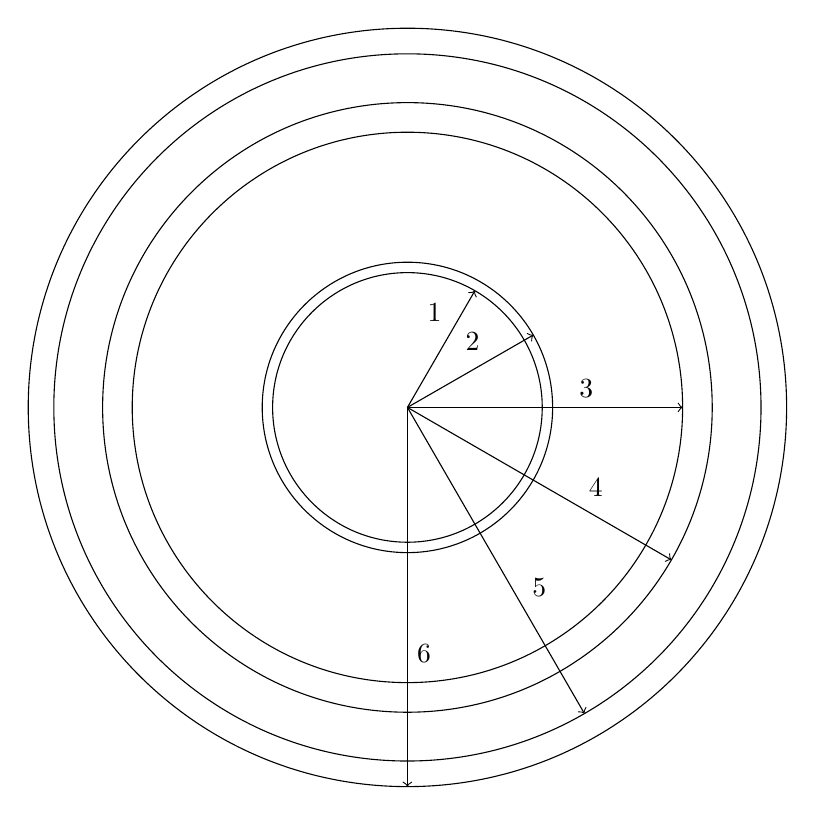
\begin{tikzpicture}[scale=8,auto]
        \draw (0,0) circle (0.214);
      \draw[->] (0,0) -- node[pos=0.65] {1} (0.107,0.185);
      \draw (0,0) circle (0.23051);
      \draw[->] (0,0) -- node[pos=0.65] {2} (0.2,0.115);
      \draw (0,0) circle (0.43688);
      \draw[->] (0,0) -- node[pos=0.65] {3} (0.437,0.0);
      \draw (0,0) circle (0.48387);
      \draw[->] (0,0) -- node[pos=0.65] {4} (0.419,-0.242);
      \draw (0,0) circle (0.56134);
      \draw[->] (0,0) -- node[pos=0.65] {5} (0.281,-0.486);
      \draw (0,0) circle (0.60198);
      \draw[->] (0,0) -- node[pos=0.65] {6} (0.0,-0.602);

      \end{tikzpicture}
      \begin{tikzpicture}
       \matrix [matrix of nodes]
      {
          Arrow & Radius (cm) & Material & \numrefheader \\
        1 & 0.21400 & \node[hyperlink node=mat_air]{Air}; & \ref{num:BPinnercladIR}\\ 
        2 & 0.23051 & \node[hyperlink node=mat_SS304]{SS304}; & \ref{num:BPinnercladOR}\\ 
        3 & 0.43688 & \node[hyperlink node=mat_helium]{Helium}; & \ref{num:BPoutercladIR}\\ 
        4 & 0.48387 & \node[hyperlink node=mat_SS304]{SS304}; & \ref{num:BPoutercladOR}\\ 
        5 & 0.56134 & \node[hyperlink node=mat_water]{Water}; & \ref{num:GTIRrad}\\ 
        6 & 0.60198 & \node[hyperlink node=mat_zirc]{Zircaloy}; & \ref{num:GTORrad}\\ 
      };
\end{tikzpicture}
\end{geoitem}
 % label: fig_ba_axials

%%%%%%%%%%%%%%%%%%%%%%%%%%%%%%%%%%%%%%%%%%%%%%%%%%%%%%%%%%%%%%%%%%%%%%%%%%%%%%%%
\subsubsection{Control Rods}
\label{sec:axial_cr}

Figure \ref{fig_cr_axials} shows the control rod axial layout, which depending
on the degree of insertion can either be occupied by the empty guide tube
pincell or the control rod pincell described in Section \ref{sec:pintypes}. The
details of insertion depend on the radial location of the specific control rod
cluster, i.e. which control or shutdown bank it belongs to. Unlike the other
axial descriptions in this section, Figure~\ref{fig_cr_axials} presents the
axial sections \emph{only} for the control rod thimble that fits inside the
guide tube. It is presented for the fully-inserted position; all intermediate
planes should be shifted according to the number of steps withdrawn, and the
appropriate axial sections created in combination with the surrounding guide
tube and grid spacer pincell.

In this model, when fully-inserted the top of the upper control rod active
absorber region should be flush with the top of the active fuel region. Control
rods are considered to be withdrawn in 228 "steps" until the active region is
drawn completely out of the active fuel region. When withdrawn 228 steps, the
bottom of the lower control rod active absorber region should be flush with the
top of the active fuel region. The total height of the lower and upper control
rod regions is 360.68 cm, meaning the step height is 1.58193 cm.

The actual axial planes used depend on the the number of steps of insertion of
the rod, and may be superseded by the highest axial plane when appropriate. In
other words, the planes presented in Figure~\ref{fig_cr_axials} should be
shifted upwards by the number of steps withdrawn times the step height.

The control and shutdown banks can have any level of partial insertion, where
the bottom tips of the rods can be at any axial step level between step 0 and
step 228. While each of these banks move their control rod clusters together,
their movement is often staggered with the other control rod banks, described in
Figure \ref{fig_cr_algorithm} with an insertion sequence example. However,
insertion levels for each individual bank are provided for most of the data
presented in this benchmark, so the algorithm in Figure \ref{fig_cr_algorithm}
may not be needed.

\begin{geoitem}{Control Rod Pin Upper Geometry}{fig_cr_pin_upper}\centering
\input{specifications/pin/figs/tikz_cr_upper}
\end{geoitem}
\begin{geoitem}{Control Rod Pin Lower Geometry}{fig_cr_pin}\centering
\input{specifications/pin/figs/tikz_cr}
\end{geoitem}
\begin{geoitem}{Control Rod Pin Spacer Geometry}{fig_cr_pin_spacer}\centering
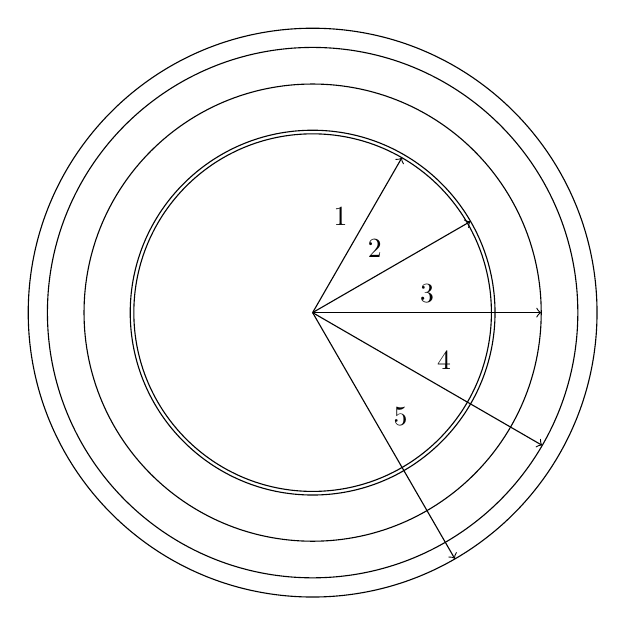
\begin{tikzpicture}[scale=6,auto]
        \draw (0,0) circle (0.37845);
      \draw[->] (0,0) -- node[pos=0.5] {1} (0.189,0.328);
      \draw (0,0) circle (0.38608);
      \draw[->] (0,0) -- node[pos=0.5] {2} (0.334,0.193);
      \draw (0,0) circle (0.48387);
      \draw[->] (0,0) -- node[pos=0.5] {3} (0.484,0.0);
      \draw (0,0) circle (0.56134);
      \draw[->] (0,0) -- node[pos=0.5] {4} (0.486,-0.281);
      \draw (0,0) circle (0.60198);
      \draw[->] (0,0) -- node[pos=0.5] {5} (0.301,-0.521);

      \end{tikzpicture}
      \begin{tikzpicture}
       \matrix [matrix of nodes]
      {
          Arrow & Radius (cm) & Material & \numrefheader \\
        1 & 0.37845 & \node[hyperlink node=mat_SS304]{SS304}; & \ref{num:CRspacerOR}\\ 
        2 & 0.38608 & \node[hyperlink node=mat_helium]{Helium}; & \ref{num:CRthimIR}\\ 
        3 & 0.48387 & \node[hyperlink node=mat_SS304]{SS304}; & \ref{num:CRthimOR}\\ 
        4 & 0.56134 & \node[hyperlink node=mat_water]{Water}; & \ref{num:GTIRrad}\\ 
        5 & 0.60198 & \node[hyperlink node=mat_zirc]{Zircaloy}; & \ref{num:GTORrad}\\ 
      };
\end{tikzpicture}
\end{geoitem}
\begin{geoitem}{Control Rod Pin Plenum Geometry}{fig_cr_pin_plenum}\centering
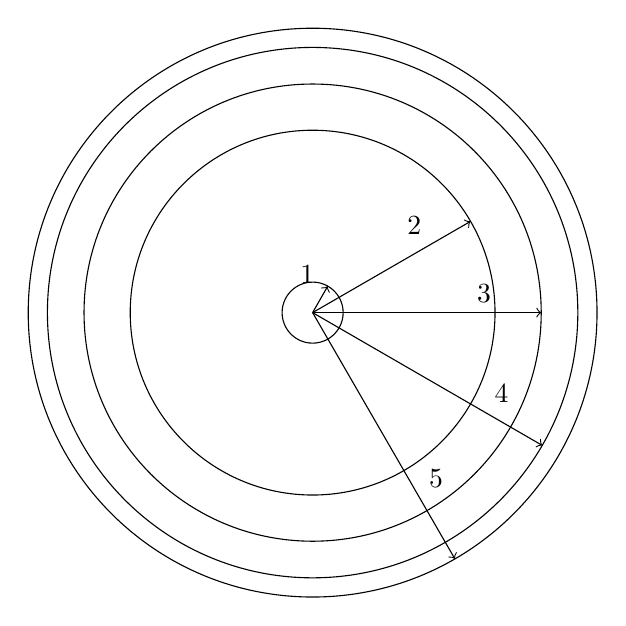
\begin{tikzpicture}[scale=6,auto]
        \draw (0,0) circle (0.06459);
      \draw[->] (0,0) -- node[pos=0.75] {1} (0.032,0.056);
      \draw (0,0) circle (0.38608);
      \draw[->] (0,0) -- node[pos=0.75] {2} (0.334,0.193);
      \draw (0,0) circle (0.48387);
      \draw[->] (0,0) -- node[pos=0.75] {3} (0.484,0.0);
      \draw (0,0) circle (0.56134);
      \draw[->] (0,0) -- node[pos=0.75] {4} (0.486,-0.281);
      \draw (0,0) circle (0.60198);
      \draw[->] (0,0) -- node[pos=0.75] {5} (0.301,-0.521);

      \end{tikzpicture}
      \begin{tikzpicture}
       \matrix [matrix of nodes]
      {
          Arrow & Radius (cm) & Material & \numrefheader \\
        1 & 0.06459 & \node[hyperlink node=mat_inconel]{Inconel}; & \ref{num:cr_plenum_spring}\\ 
        2 & 0.38608 & \node[hyperlink node=mat_helium]{Helium}; & \ref{num:CRthimIR}\\ 
        3 & 0.48387 & \node[hyperlink node=mat_SS304]{SS304}; & \ref{num:CRthimOR}\\ 
        4 & 0.56134 & \node[hyperlink node=mat_water]{Water}; & \ref{num:GTIRrad}\\ 
        5 & 0.60198 & \node[hyperlink node=mat_zirc]{Zircaloy}; & \ref{num:GTORrad}\\ 
      };
\end{tikzpicture}
\end{geoitem}
 % label: fig_cr_axials


\begin{figure}

  \centering
  \fbox{
    \begin{minipage}{6.5in}
      \textbf{Control Rod Insertion Sequence}
      ~\\
      ~\\
      Starting from all rods fully withdrawn:
      
      \begin{itemize}
        \item First D moves in alone, until it gets to 113 steps withdrawn
        \item Now D and C move together until C gets to 113 steps withdrawn \\(D is all the way in when C is at 115)
        \item Now C and B move together until B gets to 113 steps withdrawn \\(C is all the way in when B is at 115)
        \item Now B and A move together until A gets to 0 steps withdrawn \\(B is all the way in when A is at 115)
      \end{itemize}
      
      Assuming only movement of each control rod bank by one step at a time, in
      total this sequence yields 574 unique positions, which we denote with
      integer $\mathbb{S}$ steps withdrawn. If $\mathbb{S}=0$ all control rods
      are out of the core, and if $\mathbb{S}=574$ all rods are fully inserted.
      For example for normal operation with the D bank at the bite position of
      $\mathbb{S}_D = 213$ steps withdrawn, $\mathbb{S}=228-213=15$. With this
      notation, the following algorithm provides the elevation of the axial
      planes of the active region in each control rod bank ($s_i^{\mathrm{bot}}$
      and $s_i^{\mathrm{top}}$) for a given $\mathbb{S}$ with the fully inserted
      elevation $s_0$ and step width $\delta$.

      \begin{align*}
        \mathbb{S}_D &=  \max(0,~228-\mathbb{S}) \\
        \mathbb{S}_C &=  (\mathbb{S}_D<113) ~?~ \max(0,~228-\mathbb{S}+113  +3) ~:~ 228 \\
        \mathbb{S}_B &=  (\mathbb{S}_C<113) ~?~ \max(0,~228-\mathbb{S}+113\times 2+5) ~:~ 228 \\
        \mathbb{S}_A &=  (\mathbb{S}_B<113) ~?~ \max(0,~228-\mathbb{S}+113\times 3+7) ~:~ 228 \\
\\
        s_A^{\mathrm{bot}} &=  s_0 + \delta \times \mathbb{S}_A \\
        s_B^{\mathrm{bot}} &=  s_0 + \delta \times \mathbb{S}_B \\
        s_C^{\mathrm{bot}} &=  s_0 + \delta \times \mathbb{S}_C \\
        s_D^{\mathrm{bot}} &=  s_0 + \delta \times \mathbb{S}_D \\
\\
        s_A^{\mathrm{top}} &=  s_A^{\mathrm{bot}} + \delta \times 228 \\
        s_B^{\mathrm{top}} &=  s_B^{\mathrm{bot}} + \delta \times 228 \\
        s_C^{\mathrm{top}} &=  s_C^{\mathrm{bot}} + \delta \times 228 \\
        s_D^{\mathrm{top}} &=  s_D^{\mathrm{bot}} + \delta \times 228 \\
      \end{align*}
      
    \end{minipage}
  }
  
  \caption[Control rod insertion sequence and axial specification]{ Control rod insertion sequence and axial specification \cite{smith_comm}. \label{fig_cr_algorithm}}

\end{figure}


%%%%%%%%%%%%%%%%%%%%%%%%%%%%%%%%%%%%%%%%%%%%%%%%%%%%%%%%%%%%%%%%%%%%%%%%%%%%%%%%
\subsubsection{Aggregate}

By defining the full extent of the axial geometry in the pincells, several
features remain to be described or examined in the final combination of each
element of the model. In aggregate it is useful to see an exhaustive list of
all axial planes used in the model, as presented in Figure \ref{fig_all_axials}.
Control rod insertions are treated separately, as discussed in Section
\ref{sec:axial_cr}.

\begin{figure}[htbp]
    \centering
    \begin{tikzpicture}[scale=1,x=1in,y=1in]
      \draw[white] (-2.0,-2.0) rectangle (2.0,2.0);
      \node {\pgftext{\includegraphics[width=4.0in]{specifications/axial/figs/row_8_mats_axial_grids_enhanced.png}}};
      \draw[red] (1.40241130435,-2.0) -- (2.2,-2.0) -- (2.4,-2.0) -- (2.55,-2.0) node[black,right,anchor=west,font=\scriptsize] {~0.00000 ~~~~~~~~ Lowest Extent};
      \draw[red] (1.40241130435,-1.82608695652) -- (2.2,-1.82608695652) -- (2.4,-1.88235294118) -- (2.55,-1.88235294118) node[black,right,anchor=west,font=\scriptsize] {~20.0000 ~~~~~~~~ Bottom of Support Plate};
      \draw[red] (1.40241130435,-1.69565217391) -- (2.2,-1.69565217391) -- (2.4,-1.76470588235) -- (2.55,-1.76470588235) node[black,right,anchor=west,font=\scriptsize] {~35.0000 ~~~~~~~~ Bottom of Fuel Rod};
      \draw[red] (1.40241130435,-1.68045217391) -- (2.2,-1.68045217391) -- (2.4,-1.64705882353) -- (2.55,-1.64705882353) node[black,right,anchor=west,font=\scriptsize] {~36.7480 ~~~~~~~~ Bottom of Active Fuel};
      \draw[red] (1.40241130435,-1.67685130435) -- (2.2,-1.67685130435) -- (2.4,-1.52941176471) -- (2.55,-1.52941176471) node[black,right,anchor=west,font=\scriptsize] {~37.1621 ~~~~~~~~ Grid 1 Bottom};
      \draw[red] (1.40241130435,-1.66382608696) -- (2.2,-1.66382608696) -- (2.4,-1.41176470588) -- (2.55,-1.41176470588) node[black,right,anchor=west,font=\scriptsize] {~38.6600 ~~~~~~~~ Bot. of BPRA Rod};
      \draw[red] (1.40241130435,-1.65253913043) -- (2.2,-1.65253913043) -- (2.4,-1.29411764706) -- (2.55,-1.29411764706) node[black,right,anchor=west,font=\scriptsize] {~39.9580 ~~~~~~~~ Control Rod Step 0};
      \draw[red] (1.40241130435,-1.64765217391) -- (2.2,-1.64765217391) -- (2.4,-1.17647058824) -- (2.55,-1.17647058824) node[black,right,anchor=west,font=\scriptsize] {~40.5200 ~~~~~~~~ Grid 1 Top};
      \draw[red] (1.40241130435,-1.64732173913) -- (2.2,-1.64732173913) -- (2.4,-1.05882352941) -- (2.55,-1.05882352941) node[black,right,anchor=west,font=\scriptsize] {~40.5580 ~~~~~~~~ Bottom of Active Absorber};
      \draw[red] (1.40241130435,-1.63627826087) -- (2.2,-1.63627826087) -- (2.4,-0.941176470588) -- (2.55,-0.941176470588) node[black,right,anchor=west,font=\scriptsize] {~41.8280 ~~~~~~~~ Bottom of Lower Absorber (AIC)};
      \draw[red] (1.40241130435,-1.14760869565) -- (2.2,-1.14760869565) -- (2.4,-0.823529411765) -- (2.55,-0.823529411765) node[black,right,anchor=west,font=\scriptsize] {~98.0250 ~~~~~~~~ Grid 2 Bottom};
      \draw[red] (1.40241130435,-1.09791304348) -- (2.2,-1.09791304348) -- (2.4,-0.705882352941) -- (2.55,-0.705882352941) node[black,right,anchor=west,font=\scriptsize] {~103.740 ~~~~~~~~ Grid 2 Top};
      \draw[red] (1.40241130435,-0.69372173913) -- (2.2,-0.69372173913) -- (2.4,-0.588235294118) -- (2.55,-0.588235294118) node[black,right,anchor=west,font=\scriptsize] {~150.222 ~~~~~~~~ Grid 3 Bottom};
      \draw[red] (1.40241130435,-0.644026086957) -- (2.2,-0.644026086957) -- (2.4,-0.470588235294) -- (2.55,-0.470588235294) node[black,right,anchor=west,font=\scriptsize] {~155.937 ~~~~~~~~ Grid 3 Top};
      \draw[red] (1.40241130435,-0.239834782609) -- (2.2,-0.239834782609) -- (2.4,-0.352941176471) -- (2.55,-0.352941176471) node[black,right,anchor=west,font=\scriptsize] {~202.419 ~~~~~~~~ Grid 4 Bottom};
      \draw[red] (1.40241130435,-0.190139130435) -- (2.2,-0.190139130435) -- (2.4,-0.235294117647) -- (2.55,-0.235294117647) node[black,right,anchor=west,font=\scriptsize] {~208.134 ~~~~~~~~ Grid 4 Top};
      \draw[red] (1.40241130435,0.214052173913) -- (2.2,0.214052173913) -- (2.4,-0.117647058824) -- (2.55,-0.117647058824) node[black,right,anchor=west,font=\scriptsize] {~254.616 ~~~~~~~~ Grid 5 Bottom};
      \draw[red] (1.40241130435,0.263747826087) -- (2.2,0.263747826087) -- (2.4,0.0) -- (2.55,0.0) node[black,right,anchor=west,font=\scriptsize] {~260.331 ~~~~~~~~ Grid 5 Top};
      \draw[red] (1.40241130435,0.667939130435) -- (2.2,0.667939130435) -- (2.4,0.117647058824) -- (2.55,0.117647058824) node[black,right,anchor=west,font=\scriptsize] {~306.813 ~~~~~~~~ Grid 6 Bottom};
      \draw[red] (1.40241130435,0.717634782609) -- (2.2,0.717634782609) -- (2.4,0.235294117647) -- (2.55,0.235294117647) node[black,right,anchor=west,font=\scriptsize] {~312.528 ~~~~~~~~ Grid 6 Top};
      \draw[red] (1.40241130435,1.12182608696) -- (2.2,1.12182608696) -- (2.4,0.352941176471) -- (2.55,0.352941176471) node[black,right,anchor=west,font=\scriptsize] {~359.010 ~~~~~~~~ Grid 7 Bottom};
      \draw[red] (1.40241130435,1.17152173913) -- (2.2,1.17152173913) -- (2.4,0.470588235294) -- (2.55,0.470588235294) node[black,right,anchor=west,font=\scriptsize] {~364.725 ~~~~~~~~ Grid 7 Top};
      \draw[red] (1.40241130435,1.48380869565) -- (2.2,1.48380869565) -- (2.4,0.588235294118) -- (2.55,0.588235294118) node[black,right,anchor=west,font=\scriptsize] {~400.638 ~~~~~~~~ Control Rod Step 228};
      \draw[red] (1.40241130435,1.48902608696) -- (2.2,1.48902608696) -- (2.4,0.705882352941) -- (2.55,0.705882352941) node[black,right,anchor=west,font=\scriptsize] {~401.238 ~~~~~~~~ Top of Active Absorber};
      \draw[red] (1.40241130435,1.50006956522) -- (2.2,1.50006956522) -- (2.4,0.823529411765) -- (2.55,0.823529411765) node[black,right,anchor=west,font=\scriptsize] {~402.508 ~~~~~~~~ Top of Active Fuel};
      \draw[red] (1.40241130435,1.51111304348) -- (2.2,1.51111304348) -- (2.4,0.941176470588) -- (2.55,0.941176470588) node[black,right,anchor=west,font=\scriptsize] {~403.778 ~~~~~~~~ Bottom of Control Rod Plenum};
      \draw[red] (1.40241130435,1.58092173913) -- (2.2,1.58092173913) -- (2.4,1.05882352941) -- (2.55,1.05882352941) node[black,right,anchor=west,font=\scriptsize] {~411.806 ~~~~~~~~ Grid 8 Bottom};
      \draw[red] (1.40241130435,1.61012173913) -- (2.2,1.61012173913) -- (2.4,1.17647058824) -- (2.55,1.17647058824) node[black,right,anchor=west,font=\scriptsize] {~415.164 ~~~~~~~~ Grid 8 Top};
      \draw[red] (1.40241130435,1.61354782609) -- (2.2,1.61354782609) -- (2.4,1.29411764706) -- (2.55,1.29411764706) node[black,right,anchor=west,font=\scriptsize] {~415.558 ~~~~~~~~ Top of Control Rod Plenum};
      \draw[red] (1.40241130435,1.62751304348) -- (2.2,1.62751304348) -- (2.4,1.41176470588) -- (2.55,1.41176470588) node[black,right,anchor=west,font=\scriptsize] {~417.164 ~~~~~~~~ Top of Fuel Rod Plenum};
      \draw[red] (1.40241130435,1.6496) -- (2.2,1.6496) -- (2.4,1.52941176471) -- (2.55,1.52941176471) node[black,right,anchor=west,font=\scriptsize] {~419.704 ~~~~~~~~ Top of Fuel Rod};
      \draw[red] (1.40241130435,1.66549565217) -- (2.2,1.66549565217) -- (2.4,1.64705882353) -- (2.55,1.64705882353) node[black,right,anchor=west,font=\scriptsize] {~421.532 ~~~~~~~~ Top of BPRA Rod Plenum};
      \draw[red] (1.40241130435,1.67868695652) -- (2.2,1.67868695652) -- (2.4,1.76470588235) -- (2.55,1.76470588235) node[black,right,anchor=west,font=\scriptsize] {~423.049 ~~~~~~~~ Bottom of Upper Nozzle};
      \draw[red] (1.40241130435,1.75544347826) -- (2.2,1.75544347826) -- (2.4,1.88235294118) -- (2.55,1.88235294118) node[black,right,anchor=west,font=\scriptsize] {~431.876 ~~~~~~~~ Top of Upper Nozzle};
      \draw[red] (1.40241130435,2.0) -- (2.2,2.0) -- (2.4,2.0) -- (2.55,2.0) node[black,right,anchor=west,font=\scriptsize] {~460.000 ~~~~~~~~ Highest Extent};
      \draw (2.4,2.11764705882) node[left,anchor=west,font=\scriptsize] {\underline{Elevation (cm)} ~~~ \underline{Description}};

    \end{tikzpicture}


    \caption[Scale view of all axial planes.]{\emph{Left}: Scale view of row 8 axial cross section, with highlighted grid spacers and partial insertion of control rod bank D to the bite position. \emph{Right}: exhaustive list of all axial planes used in the model, excluding partial control rod insertion planes.\label{fig_all_axials}}
\end{figure} % label: fig_all_axials

\paragraph{Grid Spacers}

Nearly all axial features of the model are captured in the axial pincell
specifications. However, the stainless steel grid sleeve described in Section
\ref{sec:rad_grids} for each of the 8 grid spacers needs to be defined on the
assembly level, as it is not contained within any of the pincell elements.  The
axial planes used for the grid sleeves are the same as those used for the grids
in the pincells, as listed in Figure \ref{fig_all_axials}.

\paragraph{Nozzles and Support Plate}\label{par:nozzle}

By defining pincells as solid material pins below and
above the fuel rod regions, the model implicitly approximates the nozzle and
support plate regions as depicted in Figure \ref{fig_nozzles}.  While the axial
planes used here were taken from Source \ref{num:watts_bar}, this does not
necessarily represent the true geometry of this portion of the reactor.  However,
the special densities of water and steel for the nozzle sections were
calculated such that the mass and volume fractions of the materials are
consistent with \cite{ml033530020}. The material compositions of borated water 
and steel in the nozzle and support plate are in Material \ref{mat_water_spn}
and Material \ref{mat_ss_spn} respectively.
Thus, when modeling, the material "Nozzle / Support Plate Stainless Steel"
(\ref{mat_ss_spn}) rather than "Stainless Steel" should be used for all the fuel
rods in the upper and lower nozzle / support plate regions as depicted in Figure
\ref{fig_fuel_axials}, while the material "Nozzle / Support Plate Borated Water"
(\ref{mat_ss_spn}) rather than "Borated Water" should be used for the water in
the nozzles and support plate (Figure \ref{fig_gtu_axials}). Figures
\ref{fig_fuel_axials} through \ref{fig:tb_detail} illustrate the modeling details
with material names and colors that preserve the actual masses of material. 
Note that since the bottom nozzle and
support plate are both stainless steel, no distinction is made between the two
regions.

\begin{figure}[htpb]
  \centering
  \includegraphics[width=3in]{specifications/axial/figs/J8_nozzle.png}
  \caption{Radial picture of nozzles and support plate in aggregate model \label{fig_nozzles}}
\end{figure}

\paragraph{Top and Bottom of the Core}

For verification, Figure \ref{fig:tb_detail} shows scale
views close to the bottom and top regions of the core resulting from the
aggregate pincell specification as defined previously.

\begin{figure}[h]
    \centering
    \begin{tikzpicture}[x=1cm,y=1cm]
      \def\height{9}
      
      \draw[white] (-\height/2,\height/2) rectangle (\height*1.1,-\height*1.5);
      
      \node (toppic) at (0,0) {\includegraphics[height=\height cm]{specifications/axial/figs/axial_mats_row_8_topzoom.png}};
      \node[anchor=north] (dots) at (toppic.south) {$\vdots$};
      \node[anchor=north] (botpic) at (dots.south) {\includegraphics[height=\height cm]{specifications/axial/figs/axial_mats_row_8_botzoom.png}};

      % real geometries of the plots
      \def\realtopcenter{419.704}
      \def\realbotcenter{35.00}
      \def\realheight{57.5}
      
      \def\f{\height/\realheight}

      \def\n{20} % number of planes

      \foreach \a/\l/\c/\rc/\i in {20.0000/Bottom of Support Plate/botpic/\realbotcenter/1,
                            35.0000/Bottom of Fuel Rod/botpic/\realbotcenter/2,
                            36.7480/Bottom of Active Fuel/botpic/\realbotcenter/3,
                            37.1621/Grid 1 Bottom/botpic/\realbotcenter/4,
                            38.6600/Bottom of BPRA Rod/botpic/\realbotcenter/5,
                            39.9580/Bottom of Fully-Inserted RCCA Rod/botpic/\realbotcenter/6,
                            40.5200/Grid 1 Top/botpic/\realbotcenter/7,
                            40.5580/Bottom of BPRA Rod Absorber/botpic/\realbotcenter/8,
                            41.8280/Bottom of RCCA Rod Lower Absorber/botpic/\realbotcenter/9,
                            401.238/Top of BPRA Rod Absorber/toppic/\realtopcenter/10,
                            402.508/Top of Active Fuel/toppic/\realtopcenter/11,
                            403.778/Bottom of RCCA Rod Upper Plenum/toppic/\realtopcenter/12,
                            411.806/Grid 8 Bottom/toppic/\realtopcenter/13,
                            415.164/Grid 8 Top/toppic/\realtopcenter/14,
                            415.558/Top of RCCA Rod Upper Plenum/toppic/\realtopcenter/15,
                            417.164/Top of Fuel Rod Upper Plenum/toppic/\realtopcenter/16,
                            419.704/Top of Fuel Rod/toppic/\realtopcenter/17,
                            421.532/Top of BPRA Rod Upper Plenum/toppic/\realtopcenter/18,
                            423.049/Bottom of Upper Nozzle/toppic/\realtopcenter/19,
                            431.876/Top of Upper Nozzle/toppic/\realtopcenter/20
                            }
          \draw[red,thick] let \p{A}=(\c.west) in 
              (\x{A},\y{A}+\f*\a cm - \f*\rc cm) -- 
                  ++(\height+0.5,0) -- (\height/2+1.25,\i-\height*1.7) -- ++(0.75,0)
                      node[black,right,anchor=west,font=\scriptsize] {\l};

    \end{tikzpicture}
    
    \caption[Axial scale view of aggregate pincell model near core top and
    bottom]{Axial scale view of the model near the top and bottom of the fuel
    rods in row 8, showing pin plenums, approximated
    springs, end plugs, and structures. \emph{Blue}: water; \emph{orange}: helium;
    \emph{black}: stainless steel; \emph{dark gray}: Zircaloy; \emph{dim gray}
    Inconel; \emph{white}: air; \emph{slate gray}: nozzle / support plate
    stainless steel; \emph{steel blue}: nozzle / support plate borated water;
    \emph{green}: borosilicate glass; \emph{yellow}: fuel. \label{fig:tb_detail}}
\end{figure}



%%%%%%%%%%%%%%%%%%%%%%%%%%%%%%%%%%%%%%%%%%%%%%%%%%%%%%%%%%%%%%%%%%%%%%%%%%%%%%%%
\subsection{Materials}

  \begin{matitem}{Fuel 1.6\% Enriched}{mat_fuel16}{num:fuel16_mat}
  \centering
  \begin{tabular}{l c}
    \toprule
    Density (g/cc) & 10.31341 \\
    \midrule
    Isotope & Atom Density (atom/b-cm) \\
    \midrule
    \midrule
O16 & 4.5897e-02 \\
O17 & 1.7436e-05 \\
O18 & 9.2032e-05 \\
U234 & 3.0131e-06 \\
U235 & 3.7503e-04 \\
U238 & 2.2625e-02 \\

    \bottomrule
  \end{tabular}
\end{matitem}

\begin{matitem}{Fuel 2.4\% Enriched}{mat_fuel24}{num:fuel24_mat}
  \centering
  \begin{tabular}{l c}
    \toprule
    Density (g/cc) & 10.29748 \\
    \midrule
    Isotope & Atom Density (atom/b-cm) \\
    \midrule
    \midrule
O16 & 4.5830e-02 \\
O17 & 1.7411e-05 \\
O18 & 9.1898e-05 \\
U234 & 4.4842e-06 \\
U235 & 5.5814e-04 \\
U238 & 2.2407e-02 \\

    \bottomrule
  \end{tabular}
\end{matitem}

\begin{matitem}{Fuel 3.1\% Enriched}{mat_fuel31}{num:fuel31_mat}
  \centering
  \begin{tabular}{l c}
    \toprule
    Density (g/cc) & 10.30166 \\
    \midrule
    Isotope & Atom Density (atom/b-cm) \\
    \midrule
    \midrule
O16 & 4.5853e-02 \\
O17 & 1.7420e-05 \\
O18 & 9.1942e-05 \\
U234 & 5.7987e-06 \\
U235 & 7.2175e-04 \\
U238 & 2.2253e-02 \\

    \bottomrule
  \end{tabular}
\end{matitem}

\begin{matitem}{Fuel 3.2\% Enriched}{mat_fuel32}{num:fuel32_mat}
  \centering
  \begin{tabular}{l c}
    \toprule
    Density (g/cc) & 10.34115 \\
    \midrule
    Isotope & Atom Density (atom/b-cm) \\
    \midrule
    \midrule
O16 & 4.6029e-02 \\
O17 & 1.7487e-05 \\
O18 & 9.2296e-05 \\
U234 & 5.9959e-06 \\
U235 & 7.4630e-04 \\
U238 & 2.2317e-02 \\

    \bottomrule
  \end{tabular}
\end{matitem}

\begin{matitem}{Fuel 3.4\% Enriched}{mat_fuel34}{num:fuel34_mat}
  \centering
  \begin{tabular}{l c}
    \toprule
    Density (g/cc) & 10.35917 \\
    \midrule
    Isotope & Atom Density (atom/b-cm) \\
    \midrule
    \midrule
O16 & 4.6110e-02 \\
O17 & 1.7517e-05 \\
O18 & 9.2459e-05 \\
U234 & 6.4018e-06 \\
U235 & 7.9681e-04 \\
U238 & 2.2307e-02 \\

    \bottomrule
  \end{tabular}
\end{matitem}


  \begin{matitem}{Air}{mat_air}{num:air_mat}
  \centering
  \begin{tabular}{l c}
    \toprule
    Density (g/cc) & 0.00616 \\
    \midrule
    Isotope & Atom Density (atom/b-cm) \\
    \midrule
    \midrule
Ar36 & 7.8730e-09 \\
Ar38 & 1.4844e-09 \\
Ar40 & 2.3506e-06 \\
C12 & 6.7539e-08 \\
C13 & 7.5658e-10 \\
N14 & 1.9680e-04 \\
N15 & 7.2354e-07 \\
O16 & 5.2866e-05 \\
O17 & 2.0084e-08 \\
O18 & 1.0601e-07 \\

    \bottomrule
  \end{tabular}
\end{matitem}


  \begin{matitem}{Borosilicate Glass}{mat_borosilicate}{num:borosilicate_mat}
  \centering
  \begin{tabular}{l c}
    \toprule
    Density (g/cc) & 2.26 \\
    \midrule
    Isotope & Atom Density (atom/b-cm) \\
    \midrule
    \midrule
Al27 & 1.7352e-03 \\
B10 & 9.6506e-04 \\
B11 & 3.9189e-03 \\
O16 & 4.6514e-02 \\
O17 & 1.7671e-05 \\
O18 & 9.3268e-05 \\
Si28 & 1.6926e-02 \\
Si29 & 8.5944e-04 \\
Si30 & 5.6654e-04 \\

    \bottomrule
  \end{tabular}
\end{matitem}


  \begin{matitem}{Ag-In-Cd Control Rods}{mat_aic_rod}{num:aic_rod_mat}
  \centering
  \begin{tabular}{l c}
    \toprule
    Density (g/cc) & 10.16 \\
    \midrule
    Isotope & Atom Density (atom/b-cm) \\
    \midrule
    \midrule
Ag107 & 2.3523e-02 \\
Ag109 & 2.1854e-02 \\
Cd106 & 3.3882e-05 \\
Cd108 & 2.4166e-05 \\
Cd110 & 3.3936e-04 \\
Cd111 & 3.4821e-04 \\
Cd112 & 6.5611e-04 \\
Cd113 & 3.3275e-04 \\
Cd114 & 7.8252e-04 \\
Cd116 & 2.0443e-04 \\
In113 & 3.4219e-04 \\
In115 & 7.6511e-03 \\

    \bottomrule
  \end{tabular}
\end{matitem}


  \begin{matitem}{B4C Control Rods}{mat_b4c_rod}{num:b4c_rod_mat}
  \centering
  \begin{tabular}{l c}
    \toprule
    Density (g/cc) & 1.76 \\
    \midrule
    Isotope & Atom Density (atom/b-cm) \\
    \midrule
    \midrule
B10 & 1.5206e-02 \\
B11 & 6.1514e-02 \\
C12 & 1.8972e-02 \\
C13 & 2.1252e-04 \\

    \bottomrule
  \end{tabular}
\end{matitem}


  \begin{matitem}{Helium}{mat_helium}{num:helium_mat}
  \centering
  \begin{tabular}{l c}
    \toprule
    Density (g/cc) & 0.0015981 \\
    \midrule
    Isotope & Atom Density (atom/b-cm) \\
    \midrule
    \midrule
He3 & 4.8089e-10 \\
He4 & 2.4044e-04 \\

    \bottomrule
  \end{tabular}
\end{matitem}


  \begin{matitem}{Inconel 718}{mat_inconel}{num:inconel_mat}
  \centering
  \begin{tabular}{l c}
    \toprule
    Density (g/cc) & 8.2 \\
    \midrule
    Isotope & Atom Density (atom/b-cm) \\
    \midrule
    \midrule
Cr50 & 7.8239e-04 \\
Cr52 & 1.5088e-02 \\
Cr53 & 1.7108e-03 \\
Cr54 & 4.2586e-04 \\
Fe54 & 1.4797e-03 \\
Fe56 & 2.3229e-02 \\
Fe57 & 5.3645e-04 \\
Fe58 & 7.1392e-05 \\
Mn55 & 7.8201e-04 \\
Ni58 & 2.9320e-02 \\
Ni60 & 1.1294e-02 \\
Ni61 & 4.9094e-04 \\
Ni62 & 1.5653e-03 \\
Ni64 & 3.9864e-04 \\
Si28 & 5.6757e-04 \\
Si29 & 2.8820e-05 \\
Si30 & 1.8998e-05 \\

    \bottomrule
  \end{tabular}
\end{matitem}


  \begin{matitem}{Stainless Steel 304}{mat_SS304}{num:SS304_mat}
  \centering
  \begin{tabular}{l c}
    \toprule
    Density (g/cc) & 8.03 \\
    \midrule
    Isotope & Atom Density (atom/b-cm) \\
    \midrule
    \midrule
Cr50 & 7.6778e-04 \\
Cr52 & 1.4806e-02 \\
Cr53 & 1.6789e-03 \\
Cr54 & 4.1791e-04 \\
Fe54 & 3.4620e-03 \\
Fe56 & 5.4345e-02 \\
Fe57 & 1.2551e-03 \\
Fe58 & 1.6703e-04 \\
Mn55 & 1.7604e-03 \\
Ni58 & 5.6089e-03 \\
Ni60 & 2.1605e-03 \\
Ni61 & 9.3917e-05 \\
Ni62 & 2.9945e-04 \\
Ni64 & 7.6261e-05 \\
Si28 & 9.5281e-04 \\
Si29 & 4.8381e-05 \\
Si30 & 3.1893e-05 \\

    \bottomrule
  \end{tabular}
\end{matitem}


  \begin{matitem}{Zircaloy 4}{mat_zirc}{num:zirc_mat}
  \centering
  \begin{tabular}{l c}
    \toprule
    Density (g/cc) & 6.55 \\
    \midrule
    Isotope & Atom Density (atom/b-cm) \\
    \midrule
    \midrule
Cr50 & 3.2962e-06 \\
Cr52 & 6.3564e-05 \\
Cr53 & 7.2076e-06 \\
Cr54 & 1.7941e-06 \\
Fe54 & 8.6698e-06 \\
Fe56 & 1.3610e-04 \\
Fe57 & 3.1431e-06 \\
Fe58 & 4.1829e-07 \\
O16 & 3.0744e-04 \\
O17 & 1.1680e-07 \\
O18 & 6.1648e-07 \\
Sn112 & 4.6735e-06 \\
Sn114 & 3.1799e-06 \\
Sn115 & 1.6381e-06 \\
Sn116 & 7.0055e-05 \\
Sn117 & 3.7003e-05 \\
Sn118 & 1.1669e-04 \\
Sn119 & 4.1387e-05 \\
Sn120 & 1.5697e-04 \\
Sn122 & 2.2308e-05 \\
Sn124 & 2.7897e-05 \\
Zr90 & 2.1828e-02 \\
Zr91 & 4.7601e-03 \\
Zr92 & 7.2759e-03 \\
Zr94 & 7.3734e-03 \\
Zr96 & 1.1879e-03 \\

    \bottomrule
  \end{tabular}
\end{matitem}


  \begin{matitem}{Borated Water}{mat_water}{num:water_mat}
  \centering
  \begin{tabular}{l c}
    \toprule
    Density (g/cc) & 0.740582068 \\
    \midrule
    Isotope & Atom Density (atom/b-cm) \\
    \midrule
    \midrule
B10 & 7.9714e-06 \\
B11 & 3.2247e-05 \\
H1 & 4.9456e-02 \\
H2 & 7.7035e-06 \\
O16 & 2.4673e-02 \\
O17 & 9.3734e-06 \\
O18 & 4.9474e-05 \\

    \bottomrule
  \end{tabular}
\end{matitem}


  \begin{matitem}{Nozzle / Support Plate Borated Water}{mat_water_spn}{num:water_spn_mat}
  \centering
  \begin{tabular}{l c}
    \toprule
    Density (g/cc) & 0.981002532 \\
    \midrule
    Isotope & Atom Density (atom/b-cm) \\
    \midrule
    \midrule
B10 & 1.0559e-05 \\
B11 & 4.2716e-05 \\
H1 & 6.5512e-02 \\
H2 & 1.0204e-05 \\
O16 & 3.2683e-02 \\
O17 & 1.2416e-05 \\
O18 & 6.5535e-05 \\

    \bottomrule
  \end{tabular}
\end{matitem}


  \begin{matitem}{Nozzle / Support Plate Stainless Steel}{mat_ss_spn}{num:ss_spn_mat}
  \centering
  \begin{tabular}{l c}
    \toprule
    Density (g/cc) & 3.68384807 \\
    \midrule
    Isotope & Atom Density (atom/b-cm) \\
    \midrule
    \midrule
Cr50 & 3.5223e-04 \\
Cr52 & 6.7924e-03 \\
Cr53 & 7.7020e-04 \\
Cr54 & 1.9172e-04 \\
Fe54 & 1.5882e-03 \\
Fe56 & 2.4931e-02 \\
Fe57 & 5.7578e-04 \\
Fe58 & 7.6625e-05 \\
Mn55 & 8.0762e-04 \\
Ni58 & 2.5731e-03 \\
Ni60 & 9.9117e-04 \\
Ni61 & 4.3085e-05 \\
Ni62 & 1.3738e-04 \\
Ni64 & 3.4985e-05 \\
Si28 & 4.3711e-04 \\
Si29 & 2.2195e-05 \\
Si30 & 1.4631e-05 \\

    \bottomrule
  \end{tabular}
\end{matitem}


  \begin{matitem}{Carbon Steel}{mat_carbonsteel}{num:carbonsteel_mat}
  \centering
  \begin{tabular}{l c l c}
    \toprule
    Density (g/cc) & 7.8 \\
    \midrule
    Isotope & Atom Density (atom/b-cm) & Isotope & Atom Density (atom/b-cm) \\
    \midrule
    \midrule
Al27 & 4.3523e-05 & B10 & 2.5833e-06\\
B11 & 1.0450e-05 & C12 & 1.0442e-03\\
C13 & 1.1697e-05 & Ca40 & 1.7043e-05\\
Ca42 & 1.1375e-07 & Ca43 & 2.3734e-08\\
Ca44 & 3.6673e-07 & Ca46 & 7.0322e-10\\
Ca48 & 3.2875e-08 & Cr50 & 1.3738e-05\\
Cr52 & 2.6493e-04 & Cr53 & 3.0041e-05\\
Cr54 & 7.4778e-06 & Cu63 & 1.0223e-04\\
Cu65 & 4.5608e-05 & Fe54 & 4.7437e-03\\
Fe56 & 7.4465e-02 & Fe57 & 1.7197e-03\\
Fe58 & 2.2886e-04 & Mn55 & 6.4126e-04\\
Mo100 & 2.9814e-05 & Mo92 & 4.4822e-05\\
Mo94 & 2.8110e-05 & Mo95 & 4.8567e-05\\
Mo96 & 5.1015e-05 & Mo97 & 2.9319e-05\\
Mo98 & 7.4327e-05 & Nb93 & 5.0559e-06\\
Ni58 & 4.0862e-04 & Ni60 & 1.5740e-04\\
Ni61 & 6.8420e-06 & Ni62 & 2.1815e-05\\
Ni64 & 5.5557e-06 & P31 & 3.7913e-05\\
S32 & 3.4808e-05 & S33 & 2.7420e-07\\
S34 & 1.5368e-06 & S36 & 5.3398e-09\\
Si28 & 6.1702e-04 & Si29 & 3.1330e-05\\
Si30 & 2.0653e-05 & Ti46 & 1.2144e-06\\
Ti47 & 1.0952e-06 & Ti48 & 1.0851e-05\\
Ti49 & 7.9634e-07 & Ti50 & 7.6249e-07\\
V50 & 1.1526e-07 & V51 & 4.5989e-05\\

    \bottomrule
  \end{tabular}
\end{matitem}



%\subsection{Notes on Simplifications}
%\label{sec:simplifications}

%\subsubsection{List of Simplifications}

%A list of the main simplifications employed in the previously described model is
%presented in Table \ref{table_simps}.

%\begin{table}[htpb]

%  \caption{Key simplifications. \label{table_simps}}
%  \begin{tabular}{l}
%    \\
%    \hline\hline
%    \\ undetailed support plate, nozzles, end plugs for fuel rods, BAs, and CRs
%    \\ guessed pin plenum spring radius
%    \\ guessed shield pad thickness
%    \\ guessed RPV thickness
%    \\ no startup rods (they replace BAs in some places)
%    \\ inaccurate lower and upper core plenums
%    \\ thermal pad positioning
%  \end{tabular}

%\end{table}

%\subsubsection{Radial Symmetry}

%The only source of radial asymmetry is from the instrument tubes. If ignored,
%octant symmetry might be used to cut down the size of the problem significantly.


%\subsubsection{Grid Spacer Simplifications}

%The important thing here is to conserve the mass, so if desired the stainless
%steel and inconel can be smeared together and distributed eveny accross the
%assembly as desired, either with a similar box geometry as presented here or as
%additional rings around each of the pins.  This could confine the construction
%of the axial geometry to only the pincells, simplifying the fuel assembly
%construction.
